% !TeX encoding = UTF-8
% !TeX program = xelatex
% !TeX spellcheck = en_US

\documentclass[master]{ustcthesis}
% doctor|master|bachelor [academic|professional] [chinese|english] [print|pdf]
% [super|numebers|authoryear]

\title{面向神经网络计算库的运行时\\优化技术研究与实现}
\author{徐文明}
\major{软件工程}
\supervisor{吴锋\ 副教授}
\cosupervisor{武志辉\ 高级工程师}
% \date{二〇一九年八月十日}
% \professionaltype{专业学位类型}
% \secretlevel{秘密}        % 绝密|机密|秘密,注释本行则不保密
% \secretyear{20}           % 保密年限

\entitle{Research and Implementation of Runtime Optimization Technology for Neural Network Computing Library}
\enauthor{Xu Wenming}
\enmajor{Software Engineering}
\ensupervisor{Assoc Prof. Wu Feng}
\encosupervisor{Senior Engineer. Wu Zhihui}
% \endate{August 10, 2019}      % Today if commented
% \enprofessionaltype{Professional degree type}
% \ensecretlevel{Secret}    % Top secret|Highly secret|Secret


% 加载宏包和配置
\usepackage{graphicx}
\usepackage{subfigure}
\graphicspath{{figures/}}
\usepackage{booktabs}
\usepackage{longtable}
\usepackage[ruled,linesnumbered]{algorithm2e}
\usepackage{siunitx}
\usepackage{amsthm}
\usepackage{hyperref}


\DeclareRobustCommand\cs[1]{\texttt{\char`\\#1}}
\newcommand\pkg{\textsf}

\renewcommand\vec{\symbf}
\newcommand\mat{\symbf}
\newcommand\ts{\symbfsf}
\newcommand\real{\mathbf{R}}




\begin{document}

% 研究生论文:
%   封面,原创性声明和授权使用声明
%   frontmatter: 摘要,目录,[图、表清单],[符号说明]
%   mainmatter: 正文章节,参考文献
%   appendix: 附录
%   backmatter: 致谢,已发表论文列表
%
% 本科生论文:
%   封面
%   frontmatter: 致谢,目录,摘要
%   mainmatter: 正文章节,参考文献
%   appendix: 附录

\maketitle
\makestatement

\frontmatter
% !TeX root = ../main.tex

\begin{abstract}
  目前,深度学习加速库被广泛地用于加速神经网络应用,例如,NVIDIA和AMD公司为了加速在GPU上的神经网络运算,分别推出了自己的深度学习加速库cuDNN和MIOpen,对卷积等经典神经网络算法做了优化处理,从而加速神经网络的推理和训练速度。本文通过调研和对比当下常用的神经网络加速库的编程模型和运行流程,针对深度学习加速库的运行时系统提出了几种优化技术,并在DianNao高性能神经网络计算库(DNNCL,DianNao Neuron Network Computing Library) 上进行了实现,实践证明,这些优化技术能大幅提高神经网络应用程序在该平台上的表现。
  
  论文围绕如何设计和实现基于DianNao系列神经网络加速器的高性能计算库的运行时优化系统而展开。论文主要解决如下问题:第一,神经网络应用程序编译时间太长,编译阶段对硬件资源要求较高,不利于在嵌入式等硬件资源有限的终端部署。第二,神经网络模型的权值数据量越来越大,保存神经网络模型需要占用大量的存储空间,如何压缩神经网络模型的体积。总的来说,本文内容包括:
\begin{enumerate}
  \item 实现了一种面向神经网络模型的指令存储和加载技术,能将深度学习框架计算任务对应的指令信息和数据信息离线保存到本地离线模型文件中,然后在运行时支持从文件中加载之前编译好的指令结合当前的输入数据进行计算。
  \item 提出并实现了一种神经网络存储与识别技术,能准确的保存深度学习框架传下来的计算图信息。 
  \item 提出并实现了一种指令缓存技术,能够避免相同神经网络应用程序的重复编译。
  \item 实现了一种神经网络模型的压缩技术,对权值数据做量化处理,在保持精度损失在可接受的范围内能大幅减少神经网络模型的存储空间和部署时所占用的内存资源。
\end{enumerate}

  运行时系统是神经网络处理器软件栈中最重要的模块之一,主要负责资源管理和任务调度。本论文讨论神经网络处理器软件栈中运行时系统优化技术以及编码实现,从而提升神经网络加速库的表现。本文提出的优化技术有较强的通用性,不止限于DNNCL。
  
  \keywords{深度学习加速库;运行时优化;指令缓存;神经网络模型压缩}
\end{abstract}

\cleardoublepage

\begin{enabstract}
  Currently, deep learning acceleration libraries are widely used to accelerate neural network applications. For example, in order to accelerate neural network operations on GPUs, NVIDIA and ADM have launched their own deep learning acceleration libraries cuDNN and MIOpen, respectively. In these libraries, the reasoning and training processes of the neural network are accelerated by optimizing common algorithms, such as convolution, pooling, and activation. After investigating and comparing the programming model and running process of the commonly used neural network acceleration library, this dissertation proposes several optimization techniques for the runtime system of the deep learning acceleration library. It is implemented on the DianNao High Performance Neural Network Computation Library (DNNCL, DianNao Neuron Network Computing Library). The results show that these optimization techniques can greatly improve the performance of neural network applications on this platform.

  The dissertation revolves around how to design and implement a runtime optimization system based on the DianNao series of neural network accelerator high performance computing libraries. The dissertation mainly solves the following problems: First, the neural network application compile time is too long, and the compile stage requires high hardware resources, which is not conducive to the deployment of terminals with limited hardware resources such as embedded. This dissertation proposes the idea of ​​instruction caching and timely compilation. By means of offline caching instructions, on the one hand, it can avoid repeated compilation of the same neural network program, on the other hand, it is convenient to deploy neural network applications on embedded terminals. Second, the amount of weight data of the neural network model is getting larger and larger. The preservation of the neural network model requires a large amount of storage space, and how to compress the volume of the neural network model. In this dissertation, by reducing the weight data, the storage space occupied by the weight data is reduced, thereby reducing the volume of the neural network. In general, the runtime optimization techniques proposed in this dissertation include: 
\begin{enumerate}
  \item an instruction storage for the neural network model And the loading technology can save the instruction information and the data information corresponding to the deep learning framework calculation task to the local file offline, and then support the calculation of the previously compiled instruction combined with the current input data at the runtime to perform calculation.
  \item a neural network storage and recognition technology that accurately preserves the computational graph information passed down by the deep learning framework.
  \item Instruction cache technology, which can avoid repeated compilation of the same neural network application;
  \item A compression technique of the neural network model, which quantifies the weight data and can greatly reduce the nerve loss while maintaining the accuracy loss within an acceptable range. The storage space of the network model and the memory resources used during deployment.
\end{enumerate}
  
  The runtime system is one of the most important modules in the neural network processor software stack, and is mainly responsible for resource management and task scheduling. This dissertation discusses the runtime system optimization techniques and coding implementations in the neural network processor software stack to improve the performance of the neural network acceleration library. The optimization techniques proposed in this dissertation have strong versatility and are not limited to DNNCL.

  \enkeywords{Deep learning acceleration library; Runtime optimization;
  Instruction cache; Neural network model compression}
\end{enabstract}
\cleardoublepage

\tableofcontents
% \listoffigures
% \listoftables
% % !TeX root = ../main.tex

\begin{notation}

  \begin{notationlist}{2em}
    \item[$\displaystyle a$] The number of angels per unit area
    \item[$\displaystyle N$] The number of angels per needle point
    \item[$\displaystyle A$] The area of the needle point
    \item[$\displaystyle \sigma$] The total mass of angels per unit area
    \item[$\displaystyle m$] The mass of one angel
    \item[$\displaystyle \sum_{i=1}^n a_i$] The sum of $a_i$
  \end{notationlist}

\end{notation}



% 也可以使用 nomencl 宏包

% \printnomenclature

% \nomenclature{$\displaystyle a$}{The number of angels per unit are}
% \nomenclature{$\displaystyle N$}{The number of angels per needle point}
% \nomenclature{$\displaystyle A$}{The area of the needle point}
% \nomenclature{$\displaystyle \sigma$}{The total mass of angels per unit area}
% \nomenclature{$\displaystyle m$}{The mass of one angel}
% \nomenclature{$\displaystyle \sum_{i=1}^n a_i$}{The sum of $a_i$}


\mainmatter
% !TeX root = ../main.tex

\chapter{绪论}

AlphaGo和李世石的惊天一战,让寻常百姓都知道了AI技术的强大,AI也成为“互联网”类行业的新宠儿,被认为是下一个颠覆性的技术。人工智能领域和大数据产业有着相同的特点,需要处理的数据量极大,传统的CPU或GPU的数据处理技术已经难以满足大数据、高强度、实时性的处理需求\cite{cyj}。现在的 CPU、GPU 在进行深度学习人工神经网络处理的时候,速度慢(2012年谷歌使用1.6万个通用处理器,耗时7天才训练出一个识别猫脸的深度学习神经网络),耗能多(“阿尔法狗”下一盘棋,光电费都要3000美元)。其实,早在2006年,深度学习就开始受到科研机构、工业界的高度关注。深度学习应用要求底层芯片具备极高的并发计算能力,能在短时间内对大量训练数据进行处理\cite{szjxl}。传统的基于ARM、X86架构的通用处理器,由于其计算单元有限,无法满足深度学习领域对于算力的需求。而摩尔定律随着制程工艺接近极限(10nm以下时由量子隧穿效应造成的晶体管漏电以及光刻机精度限制)而逐渐失效,意味着在传统CPU设计逻辑上通过进一步提升制程工艺和主频很难再获得更高的算力表现\cite{ljwly}。应用于深度学习领域的硬件也CPU到向“CPU+GPU”、FPGA、ASIC多方向的发展\cite{jdk}。为了在特定的硬件平台技术深度学习应用,各大厂商组织也在积极的研究和发展自身的深度学习加速库来提高硬件平台的表现。

\section{运行时优化研究意义}

运行时优化是在程序运行的过程中采集和分析程序的运行时信息,对程序中执行频率较高的代码片断进行优化,从而加速程序运行\cite{wangjin}。相比程序生命周期中其它时期的优化(编译、装载、链接、运行后),运行时优化可提供确切的程序运行事件统计和运行环境信息,从而针对当前特定的行为模式进行特定的优化\cite{frosenb}。而其它时期的优化都只针对程序的平均行为模式,当程序运行模式偏离平均值较大时优化的效果就会大打折扣,甚至导致程序的执行时间比没有优化之前还要长\cite{gzyll}。运行时优化的这种优势,使得它在近年来得到了较为广泛的研究。

运行时系统是深度学习加速库软件栈中最重要的模块之一,优化深度学习加速库的运行时系统,对提高硬件的任务处理能力和资源利用率、节省功耗以及神经网络部署都具有十分重大的意义。

\section{国内外研究现状}

基于传统CPU体系结构,针对特定模型或特定语言,运行时优化系统已经有较为广泛的研究。例如针对特定语言的c/c++程序的运行时优化研究指出,运行时优化的关键是探测并优化热点路径,以提高代码编译指导的分支预测的正确性和局部性的性能\cite{zxj};针对java虚拟机中的运行时系统优化研究,提出了一种Java并行程序设计模型,该模型具有数据流特征,并在该模型的基础上提出了一种基于运行时信息反馈的自适应优化算法,使得运行时系统可以利用数据流程序所暴露出的数据并行性,加速程序的运行\cite{fbwcy};基于值-剖面的OpenMp运行时优化系统CCRG OpenMp指出它能够根据常见的值的组合来优化并行处理区域,并且在运行时阶段只有并行区代码需要重编译和管理。CCRG OpenMp基于动态重编译技术,避免了目前静态多版本技术的不足。同时,值-剖面的收集和分析由独立的动态优化器线程完成,降低了动态重编译引入的开销\cite{hcyxj};针对多核处理器运行时优化技术的研究指出随着多核技术的发展,运行时的优化开销将被忽略,编译优化器将成为应用程序执行中的一个服务线程\cite{lxy}。

为了加速神经网络在GPU上的运算,AMD公司和NVIDIA公司都推出了自己的深度学习加速库MIOpen\cite{miopen}和cuDNN\cite{cudnn}。MIOpen 实现了深度卷积解算器在正向和反向的优化,包括Winograd和快速傅立叶转换的卷积优化;实现了面向深度学习的广义矩阵乘算法(GEMM);Pooling、SoftMax、Active、梯度算法的批量归一化,以及LR 归一化等加速优化手段。cuDNN十分注重内存的开销,强调易用性和性能,利用将卷积计算转变成在GPU上更为友好的矩阵运算的手段,来提高卷积计算的性能,并利用高性能的并行计算来加速整个深度学习的过程。不过cuDNN和MIOpen都有一个共同的不足就是,算法支持速度较慢,只提供对非常成熟的网络算法(Convolution, Pooling, SoftMax, Active(Relu, Sigmoid, TANH))的支持,对于学术上最新提出神经网络算法,例如优化后的循环神经网络,不能及时的支持\cite{yzg}。

TensorRT\cite{tensorrt}是一款由NVIDIA推出的基于CUDA\cite{cuda}和cuDNN编程模型的推理引擎,不支持训练,只支持神经网络的推理。他的主要目标是在便于在实际的生产环境中部署深度学习应用程序,比如现在比较成熟的目标检测,图像分割,图像分类等。TensorRT之所以能提升神经网络的推理速度,主要在于其使用了两种优化手段。首先TensorRT支持神经网络的量化,支持将浮点型的神经网络转换成量化后的定点型神经网络,然后使用定点数据进行计算,减少计算量。量化会能提升计算速度,但是同时也会影响神经网络的精度,TensorRT在量化和保持精度之间达到一个理想的平衡,达到加速推断的目的。其次是TensorRT对于用户的原始网络结构进行了优化和重构\cite{tensorrtinference},优化后重构的手段主要体现在以下几个方面:1)解析网络后,消除神经网络中无用的输出层以减小计算量;2)网络结构垂直融合,简单来说将是将几个可以可以合并到一起的层融合到一个层中做,常见的是将conv、BN、Relu三个层融合为了一个层;3)网络结构水平融合,水平融合是指将输入相同,即输入是同一个张量,且执行的操作也相同的层融合一起。和其它的深度学习框架的推理速度相比,在相同的硬件条件下,TensorRT能提供10倍甚至100倍的加速,极大的提升了深度学习模型在边缘设备上的推断速度。

之后,为了解决深度学习在视频领域实时性需求,NVIDIA继续推出其新一代针对视频分析处理的高性能加速库DeepStream\cite{deepstream}。DeepStream SDK能帮助开发人员快速的构建高效、高性能的视频分析应用程序。视频分析的核心依然是图像分类、目标检测、识别和跟踪等标准的计算机视觉任务。高性能的应用程序建立在流水线上,通过将视频拆解成神经网络所需要的分辨率和格式的视频帧,从而最大化吞吐量。可扩展性要求并行处理多个视频流以获得更高的信道密度(在给定空间中处理的视频信道数量)\cite{zhangwei}。DeepStream SDK提供包含对输入视频流解码、预处理和推理的模块,所有模块都经过精细调整,以提供最大的帧吞吐量\cite{lzl}。这些模块紧密联系,以确保在正确使用数据传输和软件同步的同时获得最大的硬件并发性。不足的是,目前DeepStream只支持基于Caffe的网络\cite{lgf}。

为了解决CPU+GPU在算力、功耗和任务分配上的限制,寒武纪团队2014发表的DianNao论文提出首个多核的深度学习专用处理器架构,与主流 GPU相比,取得了21倍的性能和300倍的性能功耗比\cite{chent};2015发表的PuDianNao提出首个通用的机器学习处理器,实现了包括朴素贝叶斯、k-最近邻、 线性回归/k-均值等7种机器学习算法的兼容,平均性能与主流GPGPU相当,但面积和功耗仅为主流GPGPU百分之一\cite{liuD};2016年提出全球首个神经网络通用指令集架构,兼容十余种经典的神经网络结构,针对大规模的卷积计算,只需要一条指令就可以完成一次矩阵或向量运算\cite{lius}。随后也推出了基于自身硬件平台的机器学习加速库DNNCL,极大的提升了神经网络的推理速度\cite{cheny}。

近年来,随着深度学习算法、人工智能芯片以及深度学习加速库的快速发展,面向神经网络计算库的运行时优化技术也变得更加迫切。

\section{本文主要工作}

深度学习加速库的主要作用包括构建计算图,动态编译生成指令,拷入输入数据,任务调度、计算结果等过程,其中动态编译生成指令、拷贝输入输出数据、任务调度、计算等过程都是运行时过程。本文针对深度学习先构建计算图后计算,以及神经网络结构大多相同的特性,提出一些可以优化神经网络的运行时系统的方法,并在寒武纪深度学习加速库DNNCL的基础上实现了这些方法。实验结果表明,当采用指令缓存技术时,能避免相同神经网路的重复编译,在二次编译的情况下该方法能大幅度节省程序编译时间,提高整体的运行效率;采用权值量化技术的时候,能大幅减少神经网络模型文件的存储空间,减少神经网络部署时的内存占用。

本论文的主要内容包括:
\begin{enumerate}
  \item 调研当前主流的深度学习加速库,研究运行时优化策略。并深入理解DNNCL的编程模型、运行原理,掌握基于DNNCL构建神经网络图、编译指令、部署网络的整个流程。
  \item 实现用户计算图的快速识别并保存。计算图包含了整个神经网络具体的计算任务和对应的数据描述信息,以及计算任务的前后依赖关系。只有在识别了用户的计算意图之后,才能够进行相应的优化处理。
  \item 实现面向神经网络模型的指令存储技术。该技术能够将用户基于深度学习加速库搭建的应用程序编译之后生成的指令保存到文件中,运算时支持直接从文件中解析出指令和数据然后执行相应的计算任务。
  \item 实现面向神经网络的指令缓存技术。在1、2的基础上,如果识别出用户要执行的计算图在之前已经编译运行过,则省去当前的编译过程,直接加载之前缓存的指令,集合这次的输入数据,进行后续的计算过程。
  \item 实现了一种神经网络模型的压缩技术,对权值数据进行量化处理,在精度损失可接受的范围内,能大幅减少了神经网络模型的存储空间。
\item 在DNNCL的环境下,对这些优化方法进行编码实现,测试分析,得出结论。
\end{enumerate}

\section {本文组织结构}
本文主要描述在运行时过程中优化技术的背景,设计思路和编码实现,本文的组织结构和安排如下。

第一章:绪论。本章主要介绍和分析面向深度学习加速库中运行时优化技术的研究背景和意义,对运行时优化技术的国内外研究现状进行归纳总结,并对本文的关键内容和组织结构进行介绍说明。

第二章:深度学习加速库简介。本章主要介绍和分析现阶段主流的神经网络计算库之间的异同点,并对本文的实验环境DNNCL做了详细介绍,主要介绍其编程模型和运行流程。再此基础上,实现并验证本文的优化技术。

第三章:需求分析。本章主要从运行时优化的角度出发,结合用户的实际使用场景,分析运行时优化的功能和性能需求。

第四章:概要设计。本章主要描述软件的整体结构,进而对软件的主要模块进行独立设计。如:计算图保存模块、指令存储模块、指令缓存模块、指令加载模块、调度优化模块。

第五章:详细设计与实现。本章节主要是对神经网络框架总体架构方面的信息、系统的相关类图信息、功能模块设计等进行详细的阐述与分析,同时展示实现的效果图。

第六章:系统测试。主要是从软件测试的角度对系统的正确性、可靠性及主要功能模块进行测试分析,包括系统的测试环境的搭建、性能测试方案的设计、测试结果的分析等。

第七章:总结和展望。本章对该篇论文的主要内容进行了简要的总结,同时对运行时优化存在的不足进行分析,结合未来的发展对面向神经网络加速库运行时优化技术进行了展望。

\section {本章小结}

本章首先介绍了本论文的研究背景和研究意义,以及国内外的研究现状。关于常规应用程序或者特定语言的运行时优化技术有较多的研究,但是针对深度学习加速库运行时优化技术的研究还比较少。然后简要介绍本文的主要工作,提出并实现了一些针对深度学习加速库运行时优化的技术。最后简要介绍了本论文的组织安排,方便读者查阅。
% !TeX root = ../main.tex

\chapter{相关技术简介}
本章用3个小结来对相关的技术背景做总结介绍。在第一小结中,首先对国内外的深度学习计算库进行调研分析,分析其软件架构和整体运行流程,并从中总结出其软件设计思路和架构限制。在接下来的三节中会较为详细的介绍自己参与开发的DNNCL计算库的技术背景、编程模型和运行流程。从深度学习计算库的编程模型和运行流程上分析,提出我们的核心问题,如何优化深度学习加速库的运行时过程。

\section{深度学习计算库架构分析}
深度学习计算库的主要目的是在特定的硬件环境下,针对专门的深度学习应用,结合硬件自身的特性,通过一系列优化手段,来提升深度学习算法在硬件上的表现。目前已经有很多深度学习计算库在易用性、通用性、软件设计上都表现的很优秀。例如大家所
熟知的cuDNN计算库,利用底层GPU并行处理能力强的特性,对常见的卷积神经网络算法做了很好的优化处理,并支持多深深度学习框架。

深度学习计算库可归纳为五个层次:硬件层、驱动层、运行时层(汇聚层)、编译层、框架层(应用层)。从上到下的整体架构,如图~\ref{fig:deep-learning-struct}所示。

\begin{figure}[htb]
  \centering
  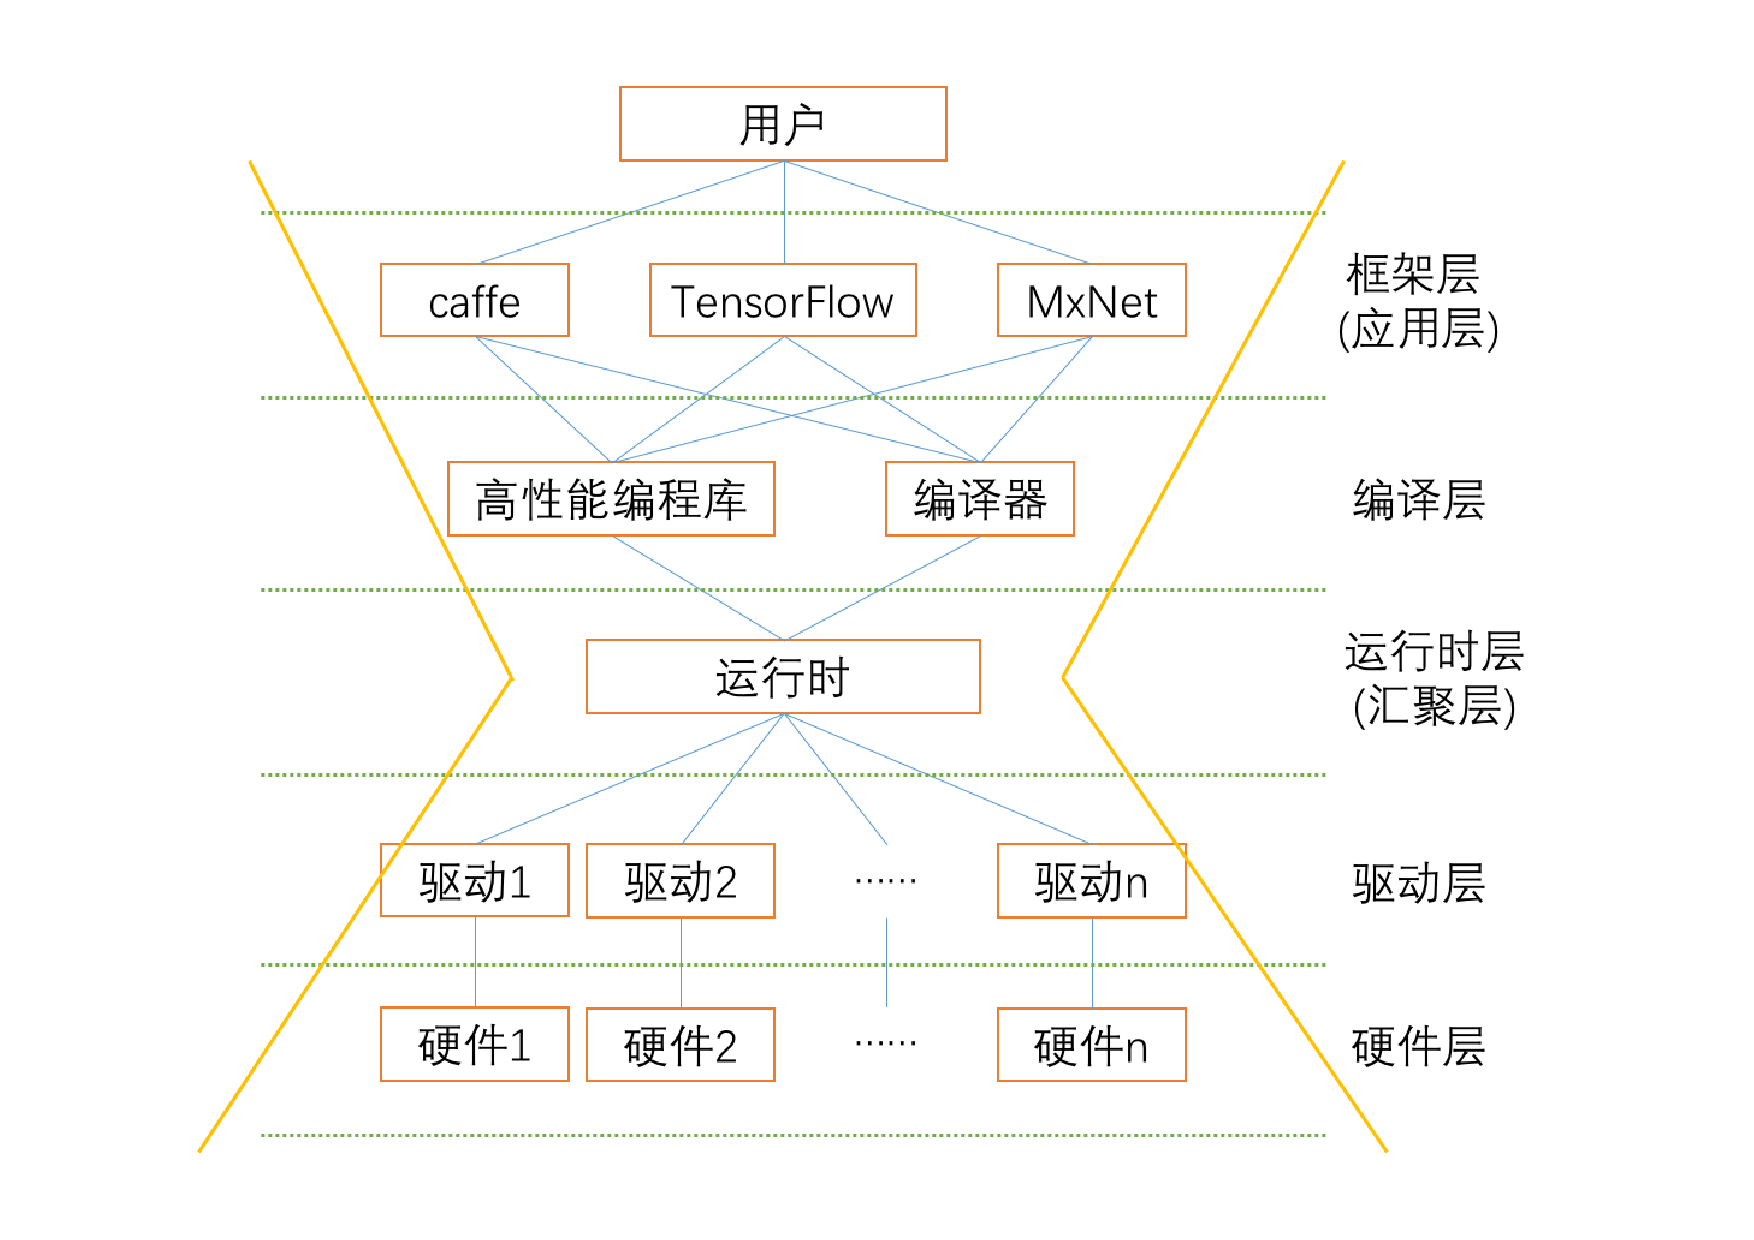
\includegraphics[width=0.6\textwidth]{deep_learning_struct.pdf}
  \caption{深度学习计算库架构图}
  \label{fig:deep-learning-struct}
\end{figure}

\subsection {硬件层}
定义:机器学习开发平台中的所有硬件设施共同构成了硬件层,包括(但不限于)主处理器(一般指CPU或通用处理器),协处理器(如基于FPGA、ASIC的加速器),存储器,输入输出设备,供电模块,以及它们的连接设备(如主板、各类桥片、总线控制器);它们共同搭建了机器学习任务开发与执行的最底层基础设施。

对上层接口:硬件层对其上层驱动层提供的信息交互接口包括(但不限于)数据接收与发送通道、控制信号接收通道、异常信号发送通道。

\subsection {驱动层}
定义:机器学习开发平台硬件层各设备所用的驱动程序称为驱动层。

功能:驱动层负责打包封装硬件层设备的基本操作,向上层运行时层提供可被调用的程序接口。基本操作包括控制数据流的输入输出(如数据拷入拷出,发送机器指令),向硬件发送控制信号(如开关设备,调整运行状态,读写寄存器),接收与处理硬件产生的异常信号(如中断处理),多任务的管理和调度等。

\subsection {运行时层(汇聚层)}
定义:运行时层是对驱动程序做进一步封装的程序,可以屏蔽底层不同硬件和驱动的差异,向上层编译层或用户提供统一的程序接口。

功能:封装上层软件不需要关心的硬件和驱动程序细节,提供机器学习任务基本操作的程序接口(如内存空间分配、数据拷贝、启动计算等),保存和加载机器学习模型及其在硬件上执行所需的机器指令等必要元素,使上层软件和用户只需要关注机器学习任务本身,而不必考虑具体硬件的差异。

\subsection {编译层}
定义:在机器学习任务中负责生成机器指令的软件称为编译层,包括编译器、针对高频算子做特殊优化的高性能编程库等\cite{randy}。

功能:接收上层框架层传入的机器学习任务的参数,编译生成硬件的二进制机器指令,传递给下层的运行时层保存下来或执行计算。

\subsection {框架层(应用层)}
定义:专注机器学习任务的算法设计,方便用户搭建自己的神经网络结构,提供便捷的训练和预测工具的软件称为框架层。

功能:接收用户设计的机器学习算法(如神经网络结构),解析出每个子任务的参数,传递给编译层生成机器指令及相关必要元素,再传递给运行时层执行计算,最终完成用户所需的机器学习任务。

可以发现整体架构呈一个沙漏形状,或称“细腰”结构,处于中间“瓶颈”环节的运行时层汇聚了上层的各类计算任务,统一了下层的所有接口,在整个机器学习开发平台的层次结构中起到了“中转站”的作用,这样设计也有利于开发的便利和保持层次的稳定,所以想要提高整体的性能,应该将重点放在提高运行时的优化上。

\section{DNNCL背景介绍}
DNNCL是DianNao系列神经网络专用处理器机器学习计算库。专用处理器顾名思义是针对某一种算法或算法家族而特殊设计的处理器, 在处理该类算法时功耗低、速度快,但是开发的成本高. 设计一个专用处理器首先需要对目标算法的特性进行详细的分析, 然后依据算法的特点来进行电路设计, 以确保最大化硬件资源利用率\cite{zhangweihua}。DianNao系列神经网络处理器从优化内存使用的角度出发而研制出来的硬件加速器, 根据机器学习算法内存分配的特点,DNNs内部设计出了不同的存储单元, 使用不同的存储单元存储不同种类数据, 最后通过流水线的方式来提高计算单元的利用率, 最终实现了以低于通用处理器约20 倍的功耗, 将计算速度提升了约117 倍, 随后使用该加速器, 设计了一个多片的DNNs 硬件系统以低于NVDIA 20M 通用图像处理器大约150 倍的功耗, 将计算速度提升了约450倍\cite{sparsenet}。

DNNCL是采用符号张量图来描述神经网络模型的结构,是一个符号式编程的库。我们知道,编程模式通常分为命令式编程(imperative style programming)和符号式编程(symbolic style programming)\cite{improgram}。命令式编程就是编写通常意义上的程序,完全按照原有逻辑执行,具有容易理解和便于调试的特点。符号式编程有用计算图来声明计算过程,编译后结合具体的输入数据执行计算。在编译阶段可以做很多的优化处理,不方便理解和调试,但能够提升内存的使用效率,加快程序运行。在现有的深度学习框架中,Torch是命令式编程的典型,完成采用命令式编程,而TensorFlow完全采用符号式编程,Caffe、MXNet则采用了两种模式混合的编程方法\cite{tensorflow}。

\begin{figure}[htb]
  \centering
  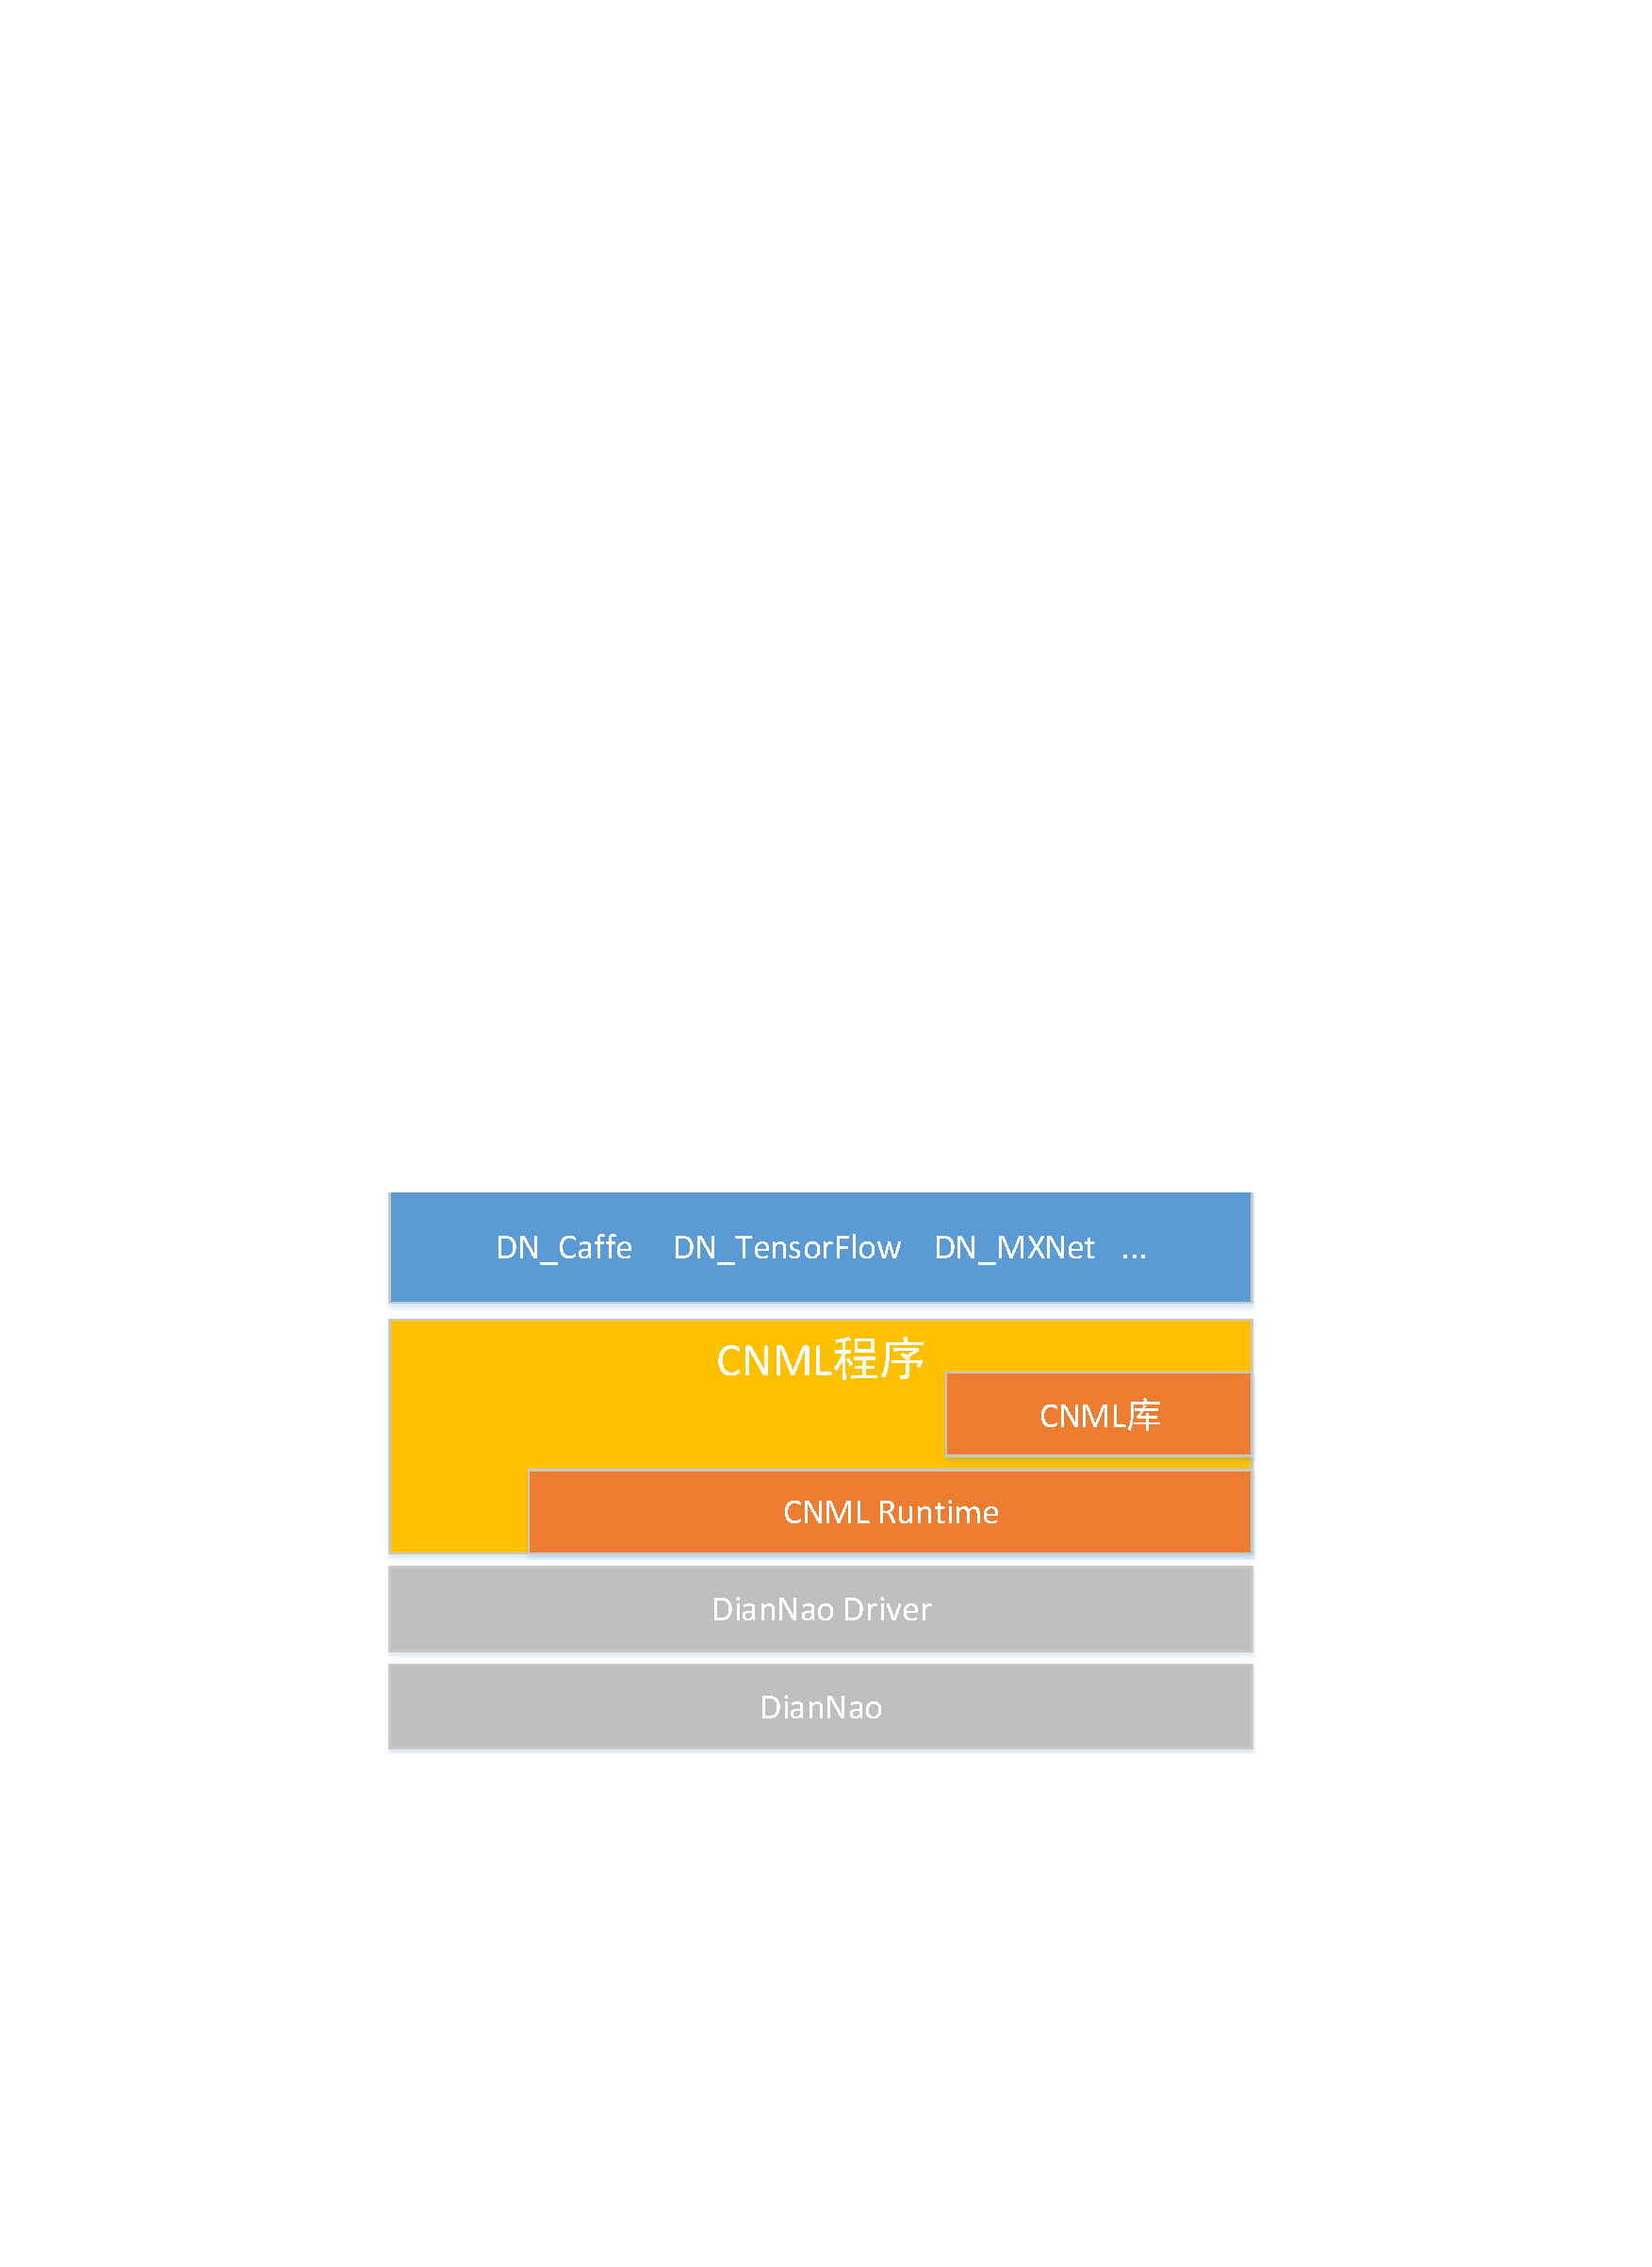
\includegraphics[width=0.4\textwidth]{dnncl_struct.pdf}
  \caption{DNNCL软件架构图}
  \label{fig:dnncl-struct}
\end{figure}

本论文所研究和实现的优化技术是基于DNNCL的,追求的目标是优化用户调用该库实现前向预测的过程。DNNCL整个架构如图~\ref{fig:dnncl-struct}所示。最底层是针对深度学习领域特点而专门研究设计的神经网路处理器;其上的驱动,直接调用各种自定义的硬件。DNNCL位于Driver之上,DNNCL的主要作用是为框架层提供各种API,其上是基于DianNao的各种深度学习框架。基于这些框架可以实现深度学习领域的各种应用,如人脸识别,自然语言处理,车牌识别等等。



\section{DNNCL编程模型介绍}
DNNCL是用数据流图做计算的,因此我们先创建一个数据流图(也称为网络结构图),如图~\ref{fig:cumputing-graph}所示,该图表示的Conv操作接收两个输入X和W做卷积计算,然后将结构传给下层的add操作,add操作接收Conv的输出和另一个输入数据B做加法运算之后再将结果传到下面的层…最终得到输出结果C。

\begin{figure}[htb]
  \centering
  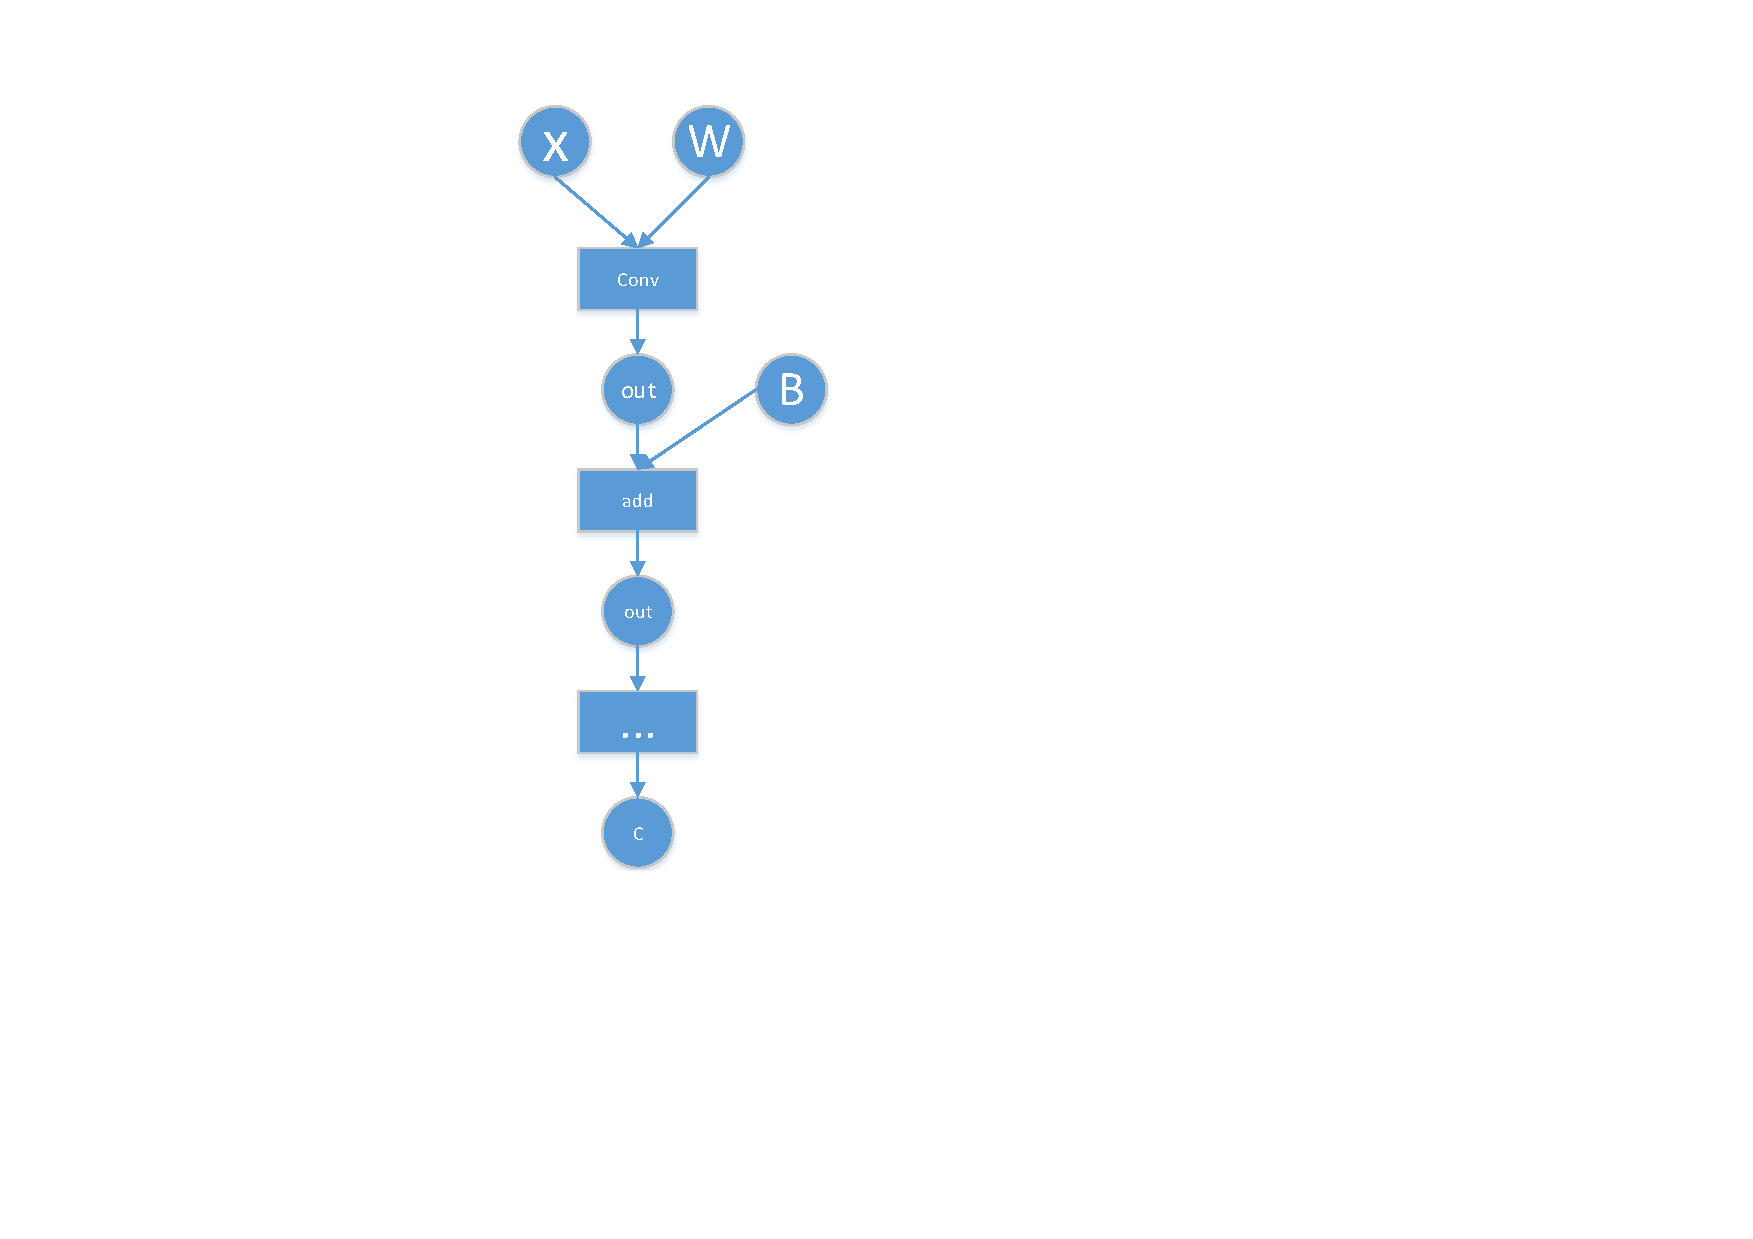
\includegraphics[scale=0.6]{computing_graph.pdf}
  \caption{计算图示例}
  \label{fig:cumputing-graph}
\end{figure}

DNNCL的数据流图是由节点(node)和边(edge)组成的有向无环图(directed acycline graph,DAG)。DNNCL由 Tensor 和 Operation 两部分组成,Tensor(张量)代表了数据流图中的边,而 Operation(操作)这个动作就代表了数据流图中节点所做的具体计算。

\subsection {边}
DNNCL的边代表数据,即张量。任意维度的数据统称为张量。在机器学习算法中,张量在数据流图中从前往后流动一遍就完成了一次前向传播(forword propagation),而残差从后向前流动一遍就完成了一次反向传播(backword propagation)。在DNNCL中,Tensor分为3类:DNNCL\_TENSOR,DNNCL\_FILTER和 DNNCL\_CONST\_TENSOR。DNNCL\_TENSOR即代表普通的输入输出;DNNCL\_FILTER即代表权值数据;DNNCL\_CONST\_TENSOR代表偏置值。DNNCL内部会根据Tensor的类型,为其分配不同的存储策略。

\subsection {节点}
图中的节点又称为算子,它代表一个操作(operation,OP),一般用来表示施加的数学运算,表~\ref{tab:compute-node}列举了一些DNNCL实现的算子。算子支持表所示的张量的各种数据属性,并且需要在建立图的时候确定下来。

\begin{table}[htb]
  \centering\small
  \caption{常见运算节点举例}
  \label{tab:compute-node}
  \begin{tabular}{ll}
    \toprule
    节点类别   &  示例                                     \\
    \midrule
    数学运算操作 & Add、Subtract、Multiply、Div、Exp、Log、Greater、Less... \\
    数组运算操作 & Concat、Split、Slice、Shape、Rank... \\
    矩阵运算操作 & MatMul、Transpose...     \\
    神经网络构建操作 & SoftMax、Convolution2D、Relu、Sigmoid、pool... \\
    \bottomrule
  \end{tabular}
\end{table}

\subsection {图}
把操作任务描述成有向无环图。DNNCL构建图的方法分为三步,第一步是创建边;第二步,将边作为创建节点的输入输出参数来创建节点;第三步通过接口将节点连接在一起构成图。

\subsection {队列}
启动图的第一步是创建一个队列(queue)对象。队列提供在图中执行操作的一些方法。一般的模式是,建立队列,此时会生成一个计算任务的队列,在队列中添加计算图,然后执行。在调用前向计算接口来执行图时,需要填充一些输入Tensor;取回的结果类型根据输入的类型而定。

\subsection {设备}
设备(device)是指执行计算任务的硬件,拥有自己的地址空间并可以执行计算任务,DNNCL为了实现分布式执行操作,充分利用计算资源,可以明确指定当前的操作在哪个设备上执行。

\subsection {内核}
操作(operation)是对抽象操作(如 matmul 或者 add)的一个统称,而内核(kernel)则是能够运行在特定设备(如 CPU、GPU)上的一种对操作的实现。因此,同一个操作可能会对应多个内核\cite{dongmian}。当自定义一个操作时,需要把新操作和内核通过注册的方式添加到系统中。

\section{DNNCL运行流程}
DNNCL是个声明式编程库,运行流程如图~\ref{fig:dnncl-run-process}所示。

\begin{figure}[htb]
  \centering
  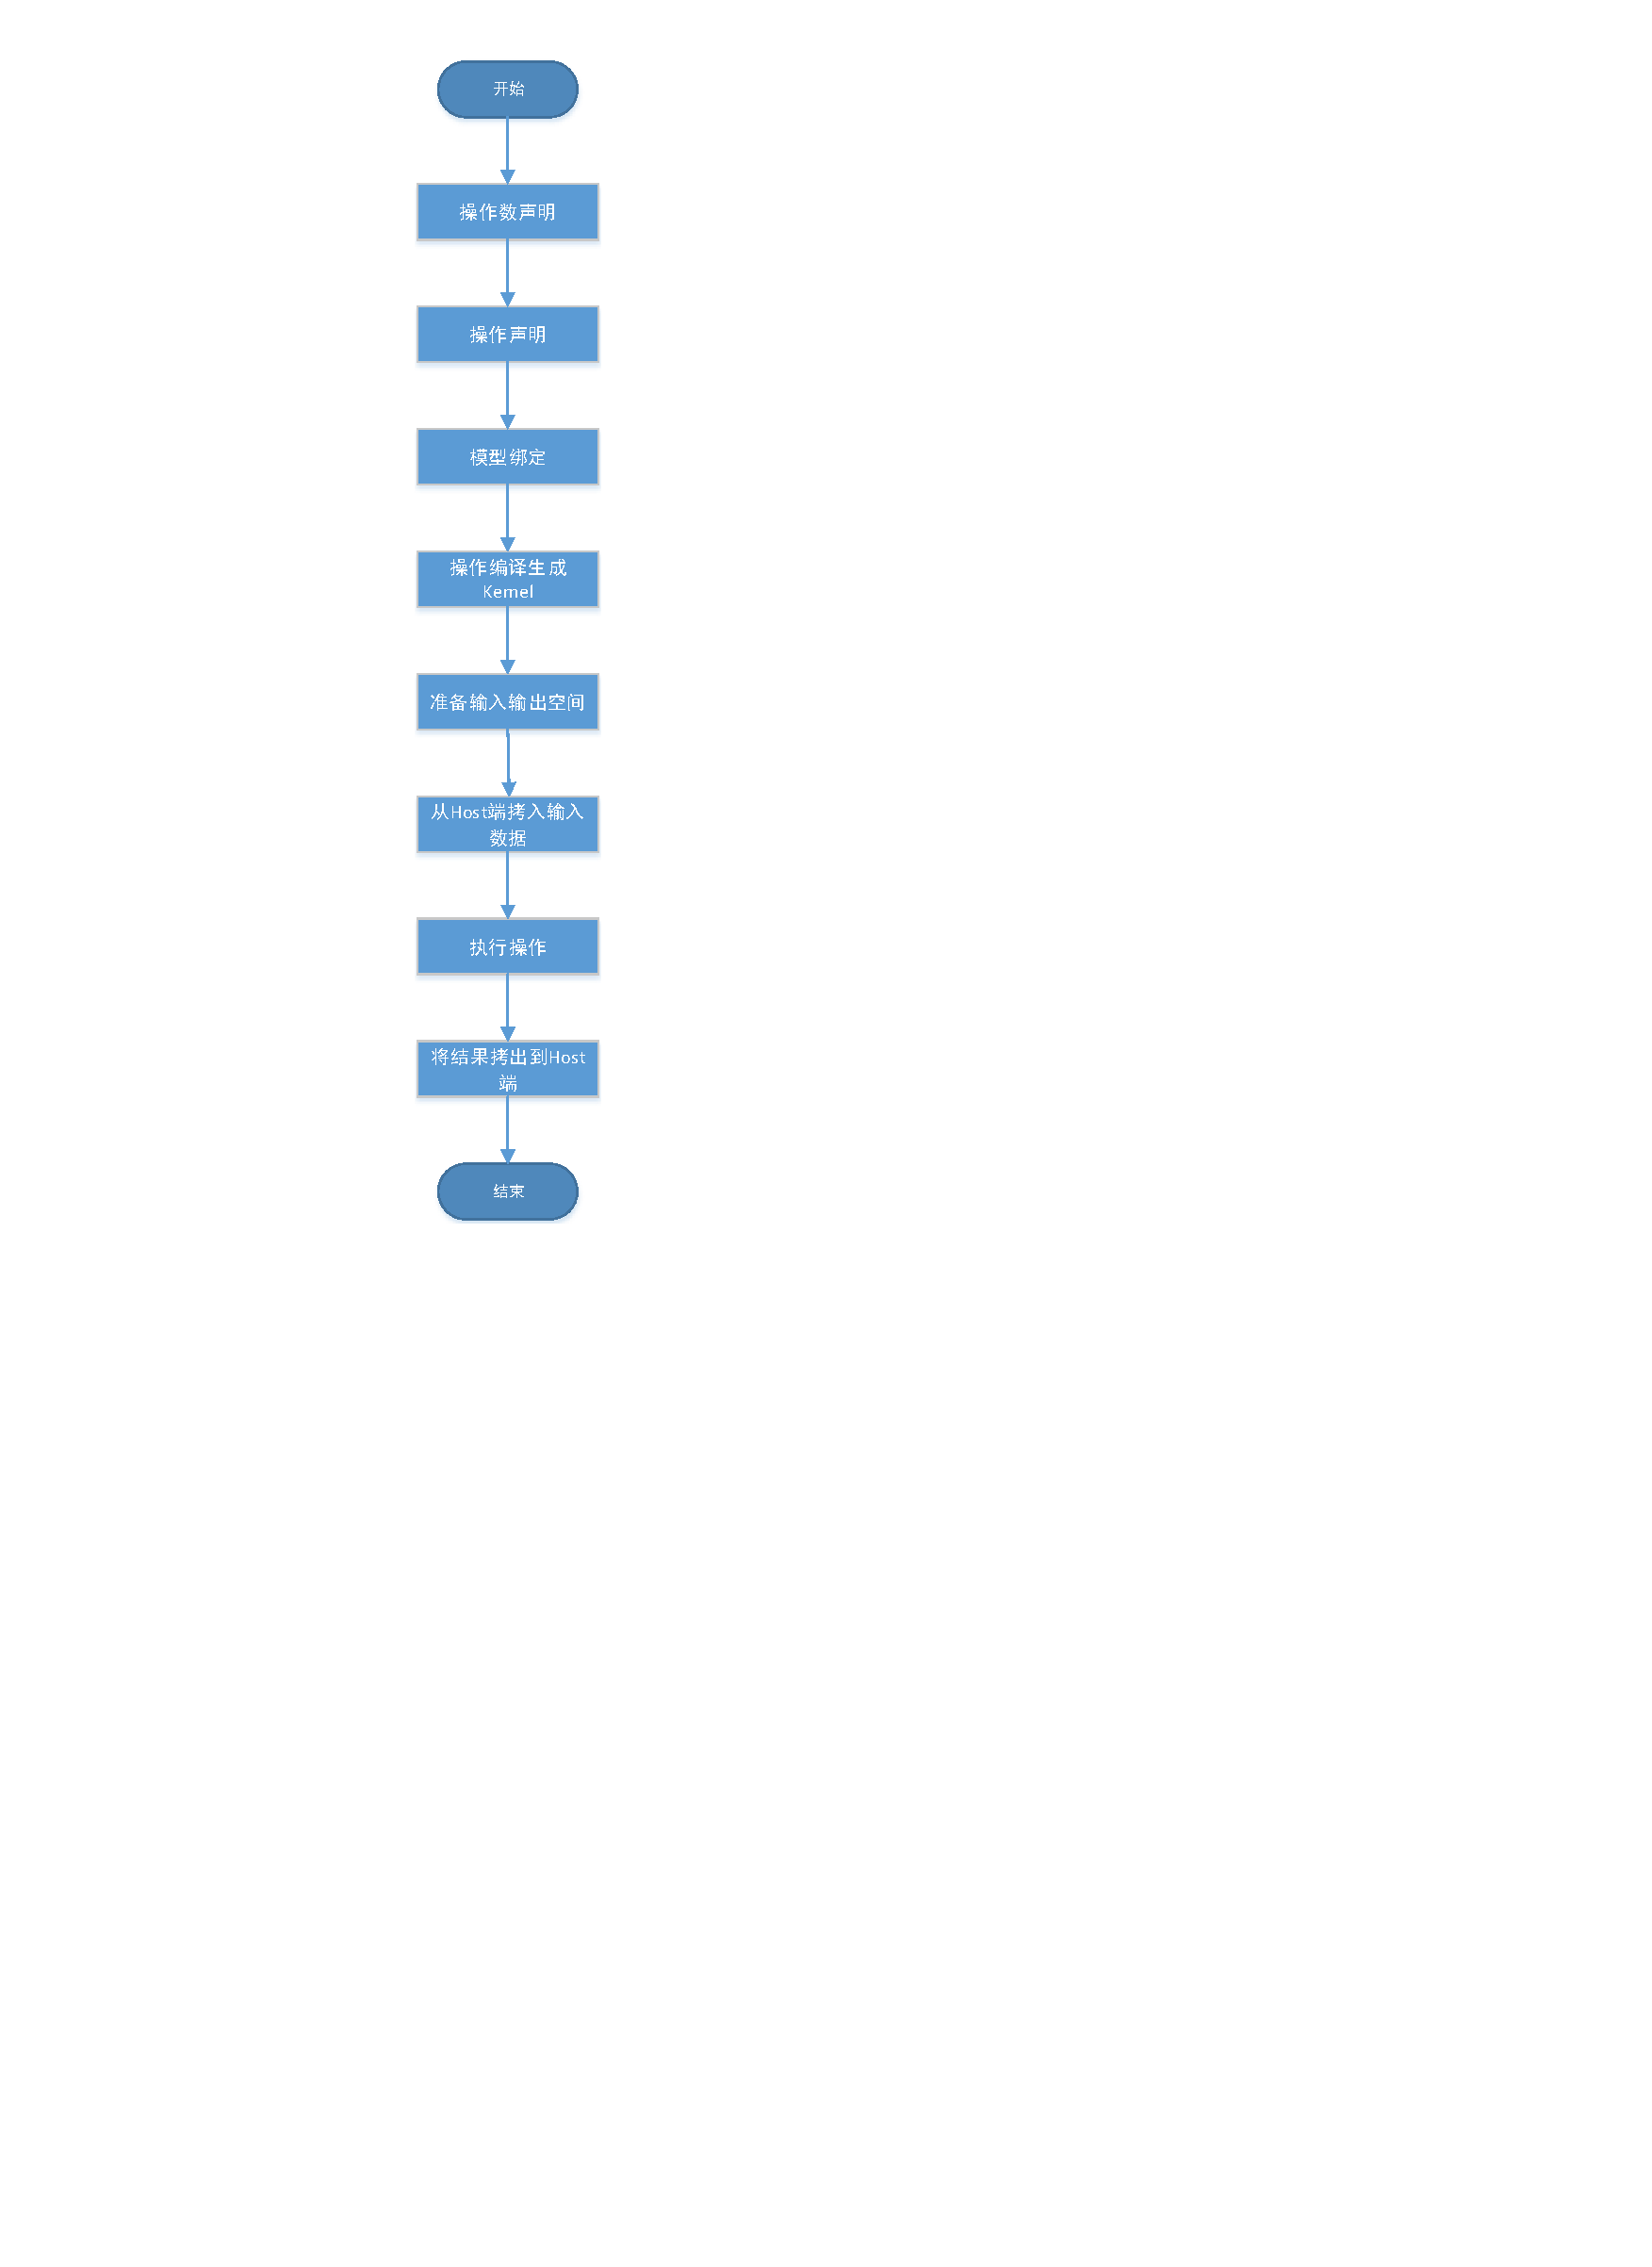
\includegraphics[width=0.15\textwidth]{dnncl_run_process.pdf}
  \caption{DNNCL运行流程图}
  \label{fig:dnncl-run-process}
\end{figure}

对于单个操作的运算,主要分为以下几步:操作数声明、操作声明、模型绑定、操作编译、Host 端准备输入输出空间并为该输入空间赋予相应的值、Device 端准备输入输出空间,拷贝 Host 端的输入数据到 Device 端,操作具体执行,拷贝 Device 端的输出数据到 Host 端。

操作数声明:即创建Tensor,设置Tensor属性,包括Tensor类型,数据维度、数据类型、数据摆放顺序等信息。数据摆放顺序指的是host端的图片数据在内存中是按哪种顺序摆放的,例如NCHW和NHWC等,N代表图片的数量,C代表图片的通道,H代表图片的高,W代表图片的宽。操作声明:即创建Operation,Op的输入包括创建的Tensor和计算所需的一些额外参数信息。

模型绑定:即构建计算图的过程,将单Op连接到一个构成一个复杂的融合Op。一个复杂的神经网路就是一个或者多个融合Op。

操作编译:即根据具体的硬件平台将操作编译生成能在设备上运行的Kernel的过程。在编译过程中能做些优化措施,例如图优化,数据量化等。在该阶段的优化是透明的,对用户不可见。

准备输入输出空间:即host端和device端准备输入输出数据的空间。在神经网络的推理过程中,只有神经网络的输入数据是动态变化的,其余参与计算的静态数据(filter和bias)是保持不变的。在编译过程中,静态数据会被提前保存到kernel中,所以在实际计算的过程中,只需要为输入数据动态分配空间。

从Host端拷入输入数据到Device端:即将Host端的输入数据拷贝到Device端的过程。由于DNNCL的设备端只支持以一种特定的数据摆放顺序进行计算,但是Host端数据顺序可能有多种,所以在拷贝数据的过程中还涉及到转数的过程。即将host端的数据按照Device端的顺序重新排布。

执行操作:即启动设备,执行具体计算的过程。

拷贝Device端计算结果到Host端:即将Device端的计算结果拷贝到Host端的过程,和拷贝输入数据一样,该过程也涉及到转数的过程。

\section {本章小结}
本章详细介绍了本文实验平台的基础知识,包括DNNCL的设计理念、编程模型和运行流程。DNNCL库是声明式编程,将计算图定义和图计算完成分开,便于优化神经网络的计算过程来提升计算速度。编程模型中简要介绍了库中的边、节点、图、设备、会话、内核等核心概念,简要说明了如何去构建计算图。在运行流程一节中简要介绍了用户在DNNCL上完成神经网络计算所进行的主要步骤,包括声明操作数、声明操作、模型绑定、编译操作、拷贝 Host 端的输入数据到 Device 端、执行具体操作,拷贝 Device 端的输出数据到 Host 端等过程。

% !TeX root = ../main.tex

\chapter{需求分析}
本章在上一章介绍的DNNCL深度学习计算库上测试不同的神经网络,探究运行时的状态,从而找到运行时优化的切入点。从需要实现什么入手,对本系统的需求进行分析和整理,确定本系统需要实现哪些功能以及需要满足哪些非功能性需求。然后将需求逐步求精和细化,分析各种可能的解法,并且分配给各个软件元素。

\section{需求挖掘}
本系统的主要目标是优化深度学习库的运行时过程,而运行时优化少不了对热点路径的探测和优化。通过在DNNCL库上运行经典神经网络,对运行时各个阶段的时间进行统计分析。包括拷贝输入输出时间、动态编译时间、加载Kernel的时间、IPU执行计算的时间。输入输出时间代表将数据输入数据从主机端考入到设备端和将结果从设备端拷出的时间;动态编译时间指的是从深度学习库拿到用户搭建的计算图后编译生成Kernel的时间;加载Kernel的时间指的是将编译好的Kernel从CPU端加载到设备端所用的时间;IPU执行计算的时间指的是启动IPU执行推理过程的时间。统计发现,绝大多数网络中,动态编译时间的开销占到了整个推理过程的99\%左右。也就是说动态编译的时间的占了整个推理时间的大头,所以想要增加神经网络的表现性能,可以将目标放在优化编译阶段。

由于DNNCL是由C和C++语言实现,C/C++程序是静态编译优化的典型代表,并且静态优化技术的成熟,使得静态优化对程序性能提升的空间越来越小。所以这里考虑用动态重编译技术来优化编译过程。结合神经网络应用的使用场景不难发现,一个相同的神经网络往往在短时间内被多次使用。而现在的模式下,每运行一次神经网络就会重新编译生成一次指令。每次都会花费很多时间在编译指令上,特别是在一些端设备上,长时间的等待是无法接受的。因此可以想办法优化编译的过程,避免相同神经网络的重复编译过程,减少调用同一程序带来的编译开销。
另外由于神经网络大多结构相同,针对不同的应用场景只是只有权值等数据发生了变化。如果有一份编译好的指令,支持动态更新里面的静态数据,那也可以省略掉重复编译的开销。

随着卷积神经网络模型堆叠的层数越来越多,网络模型的权重参数数量也随之增长,并且现在神经网络的权值数据大部分是用单精度4字节的float32或者双精度8字节的float64表示,所以网络模型存储体积越来越大。如果能降低模型的存储空间将更有助于将神经网络模型部署到通用的嵌入式移动平台。

\section {功能性需求}
从挖掘的需求分析,要避免重复编译带来的开销,应该将编译好的指令缓存起来。要想实现指令缓存,本优化系统则应该具备以下功能:
\begin{enumerate}
  \item 编译入口接收到的是用户构建的计算图,所以应该具有保存计算图、计算图识别的功能。
  \item 想要避免重复编译,则要想办法保存编译好的指令并且之后能解析指令文件,所以应该具有指令保存、指令加载的功能。
  \item 二进制机器代码是和硬件的驱动版本相关的,当驱动更新时,二进制代码也会发生变化,所以还应该就有向前兼容性
  \item 缓存的指令占用存储空间,不能无限制的增长,因此需要设置存储上限和合理的查找和替换策略。
\end{enumerate}

想要实现静态数据的更新,不仅需要识别出静态数据发生了变化,还需要识别出哪个静态数据发生了变化。所以应该就有静态数据标识,静态数据对比,静态数据替换的功能。

为了降低模型的存储空间达到模型压缩加速的目的,可以对参数进行量化。参数量化可以利用定点数表示浮点数的方式来实现,用1字节的int8来表示4字节的float32能节省大约4倍的存储空间。量化的过程中会带来一定的精度损失,但是可以减少存储空间、加速计算,带来性能方面的大幅提升。结合以上的分析,得到图~\ref{fig:user-need}所示用例图。

\begin{figure}[htb]
  \centering
  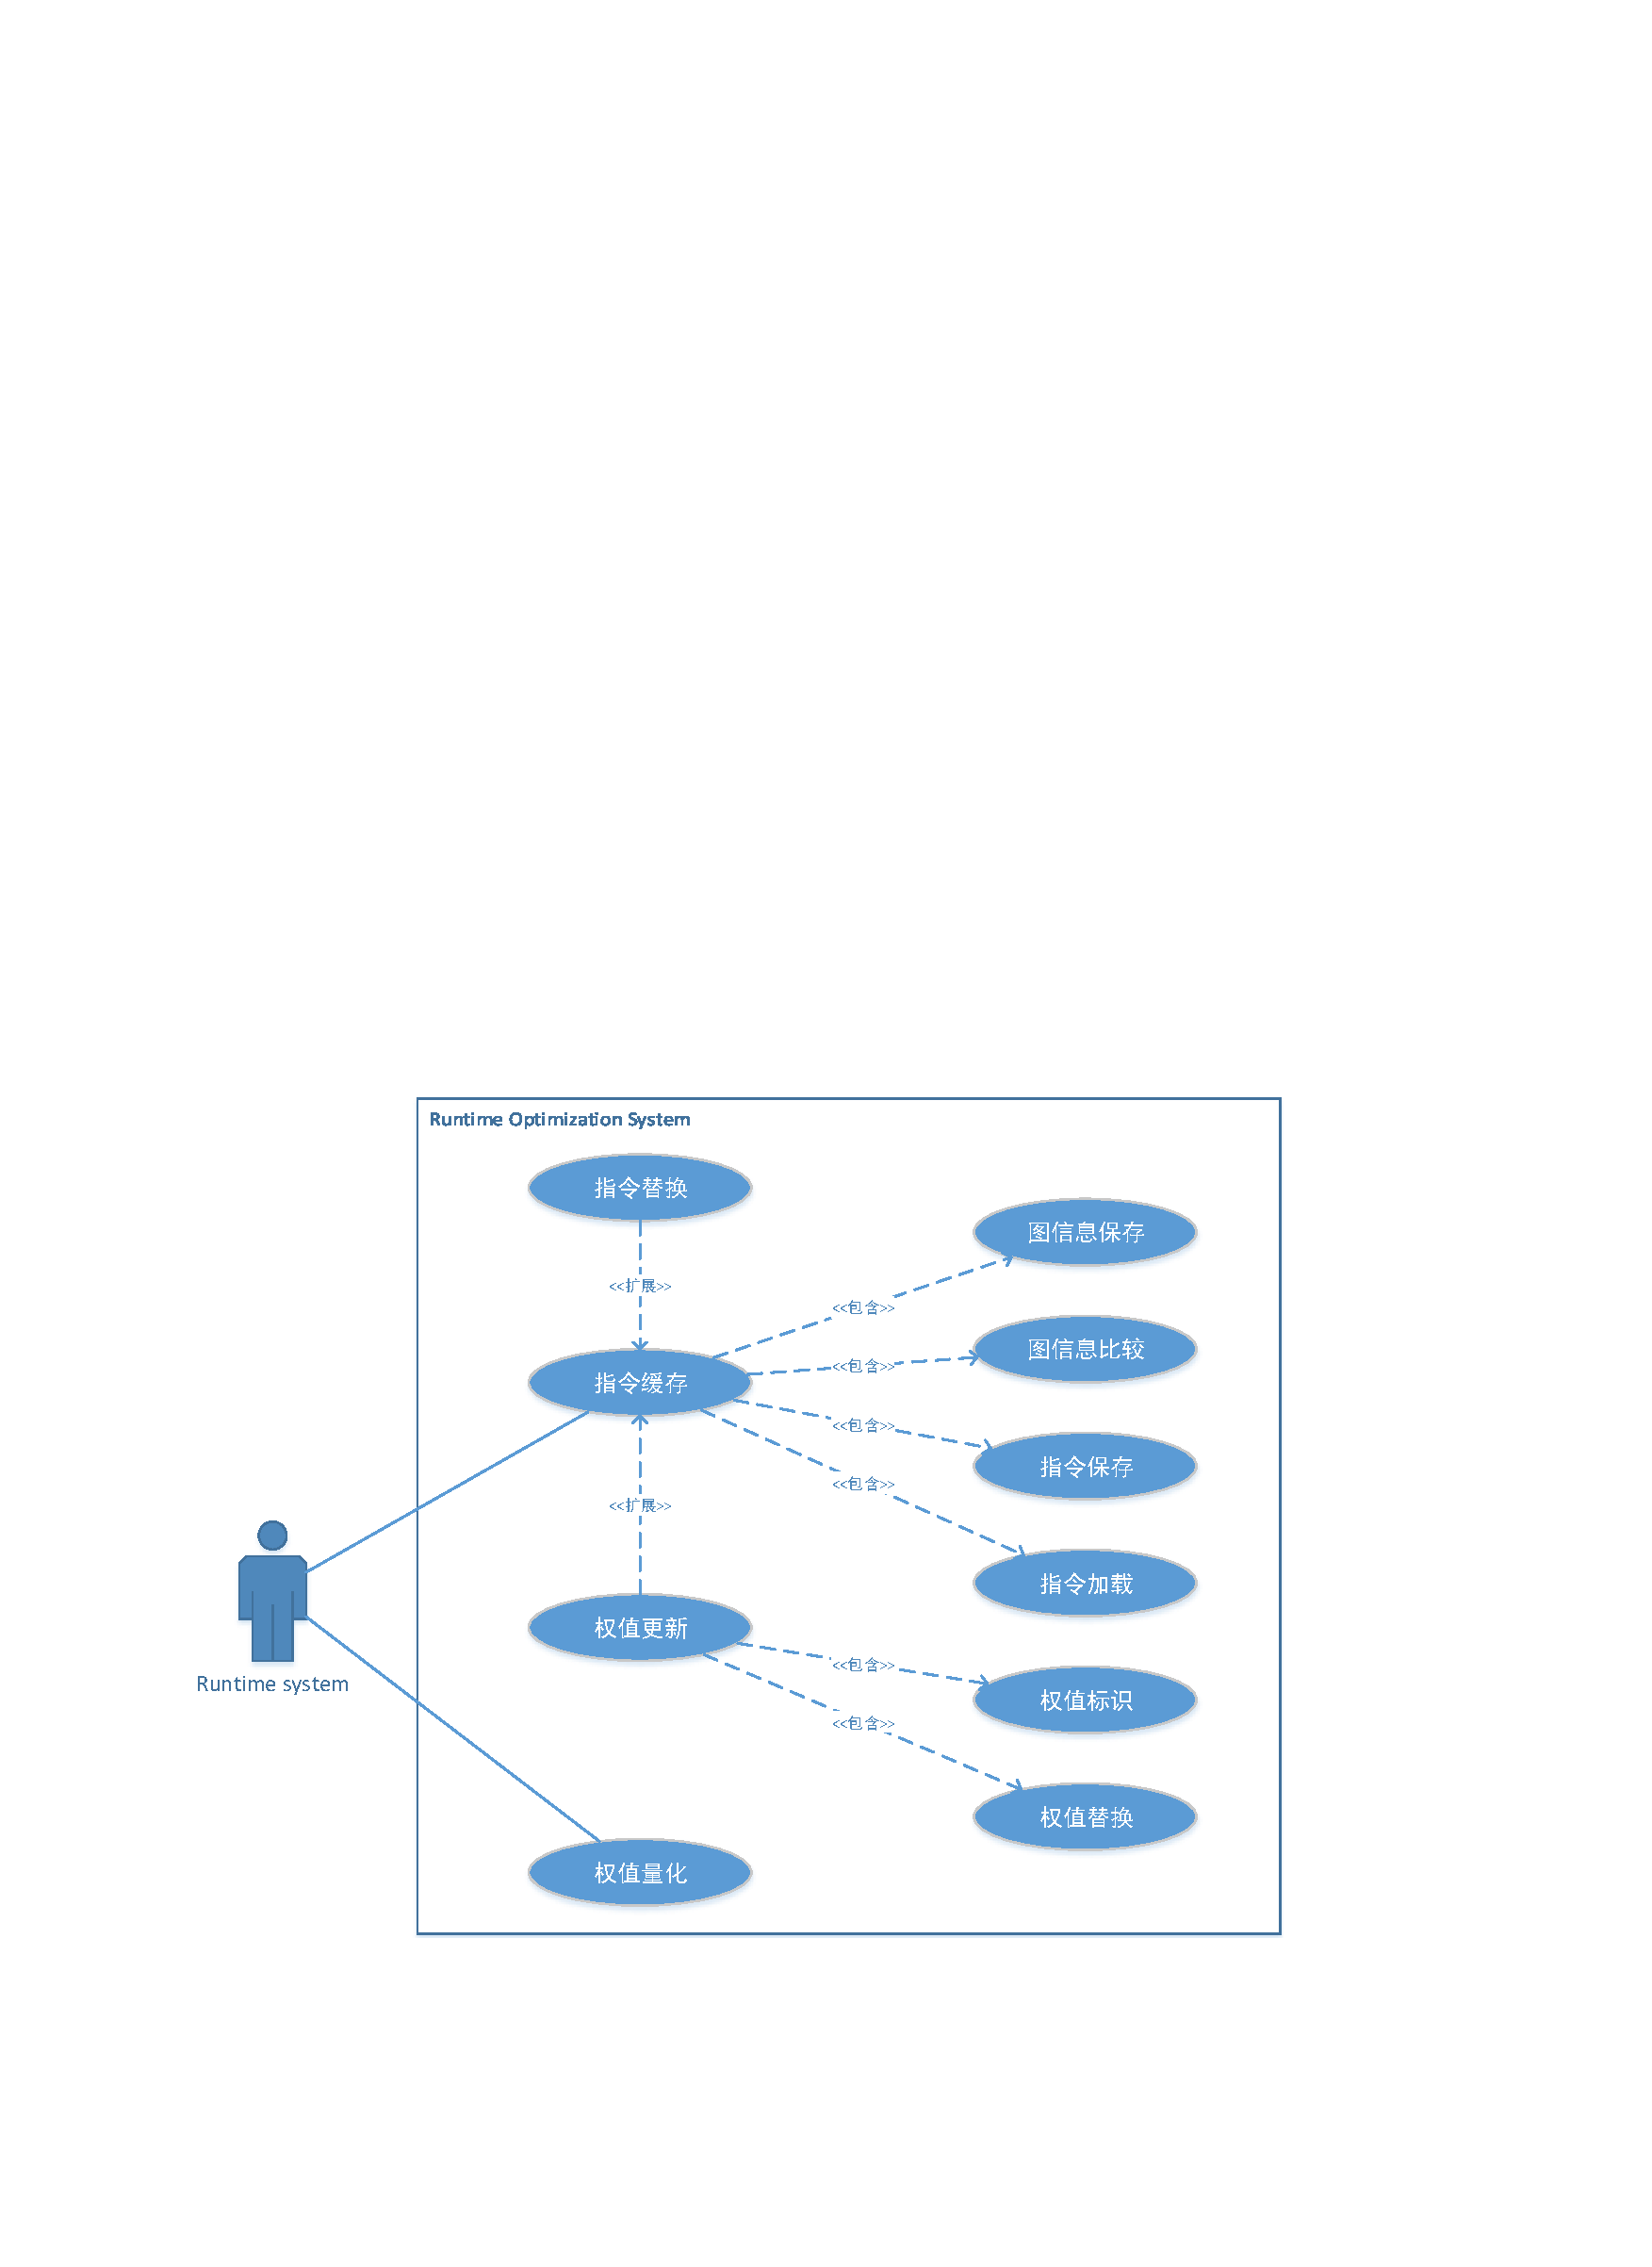
\includegraphics[width=0.6\textwidth]{user_need.pdf}
  \caption{运行时优化系统用例图}
  \label{fig:user-need}
\end{figure}

运行时优化系统属于对运行时的优化,对外用户不可见,通过特定的方式是功能生效。运行时优化系统应该具备以下功能:
\begin{enumerate}
  \item 指令缓存:指令缓存的功能中包含四个必不可少的功能,计算图信息保存、计算图信息比较、指令保存以及指令加载,有两个拓展功能,指令替换和权值更新。当缓存空间已满时需要用到指令替换功能,当计算图结构相同而权值信息不同时需要用到权值更新功能。权值更新的实现必须依赖权值标识和权值替换。
  \item 权值量化:权值量化功能,通过压缩神经网络权值信息的存储空间,达到减少神经网络模型存储空间的目的。
\end{enumerate}

\section {非功能性需求}

\subsection {时间特性}
本系统的目的是节省深度学习加速库运行时的开销,但是在实现优化的过程中,不可避免的会引入新的开销,例如计算图识别、缓存查找替换、静态数据更新的过程。但总的原则应该是优化后的时间开销不能比优化之前的时间开销还大,理想状态应该是能大幅缩减原神经网络运行过程的时间开销。

\subsection {用户友好性}
本系统优化的过程应该对用户透明,但是部分功能应该由用户根据自己的实际情况来决定是否采用优化过程。即使开启了性能优化模式,某些功能参数也应该能由用户根据自己的实际情况来设置。例如指令缓存空间的大小和路径,应该允许用户应该根据自己实际存储空间大小合理设置。是否开启参数量化功能也应该由用户根据精度优先还是性能优先决定。

\section {本章小结}
本章从需要“实现什么”入手,首先采用运行时优化的常规手段,对神经网络应用程序的热点路径进行探究,测试发现时间主要耗在编译阶段,因此挖掘出优化编译过程的需求。从该需求出发,结合神经网络应用的特点,提出解决方案,最终拓展出指令缓存、权值更新、指令替换、权值量化等多方面更加具体的需求。
% !TeX root = ../main.tex

\chapter{概要设计}
本章在第3章需求分析的基础上,对运行时优化系统的设计进行初步介绍。首先将大的需求解耦,划分成不同的模块,然后对模块的内部功能和对外接口进行设计,相互配合依赖,达到系统最终的目的。

\section {总体设计}
\subsection {主流程优化}
分析DNNCL的运行流程,我们可以将其总结概括为以下几个步骤:构建计算图,动态编译,拷入数据,执行计算,拷出结果。结合需求分析,决定将优化措施分布在这几个步骤之中。如图~\ref{fig:main-process}所示,蓝颜色的是原流程的内容,黄色的表示优化的内容。

\begin{figure}[htb]
  \centering
  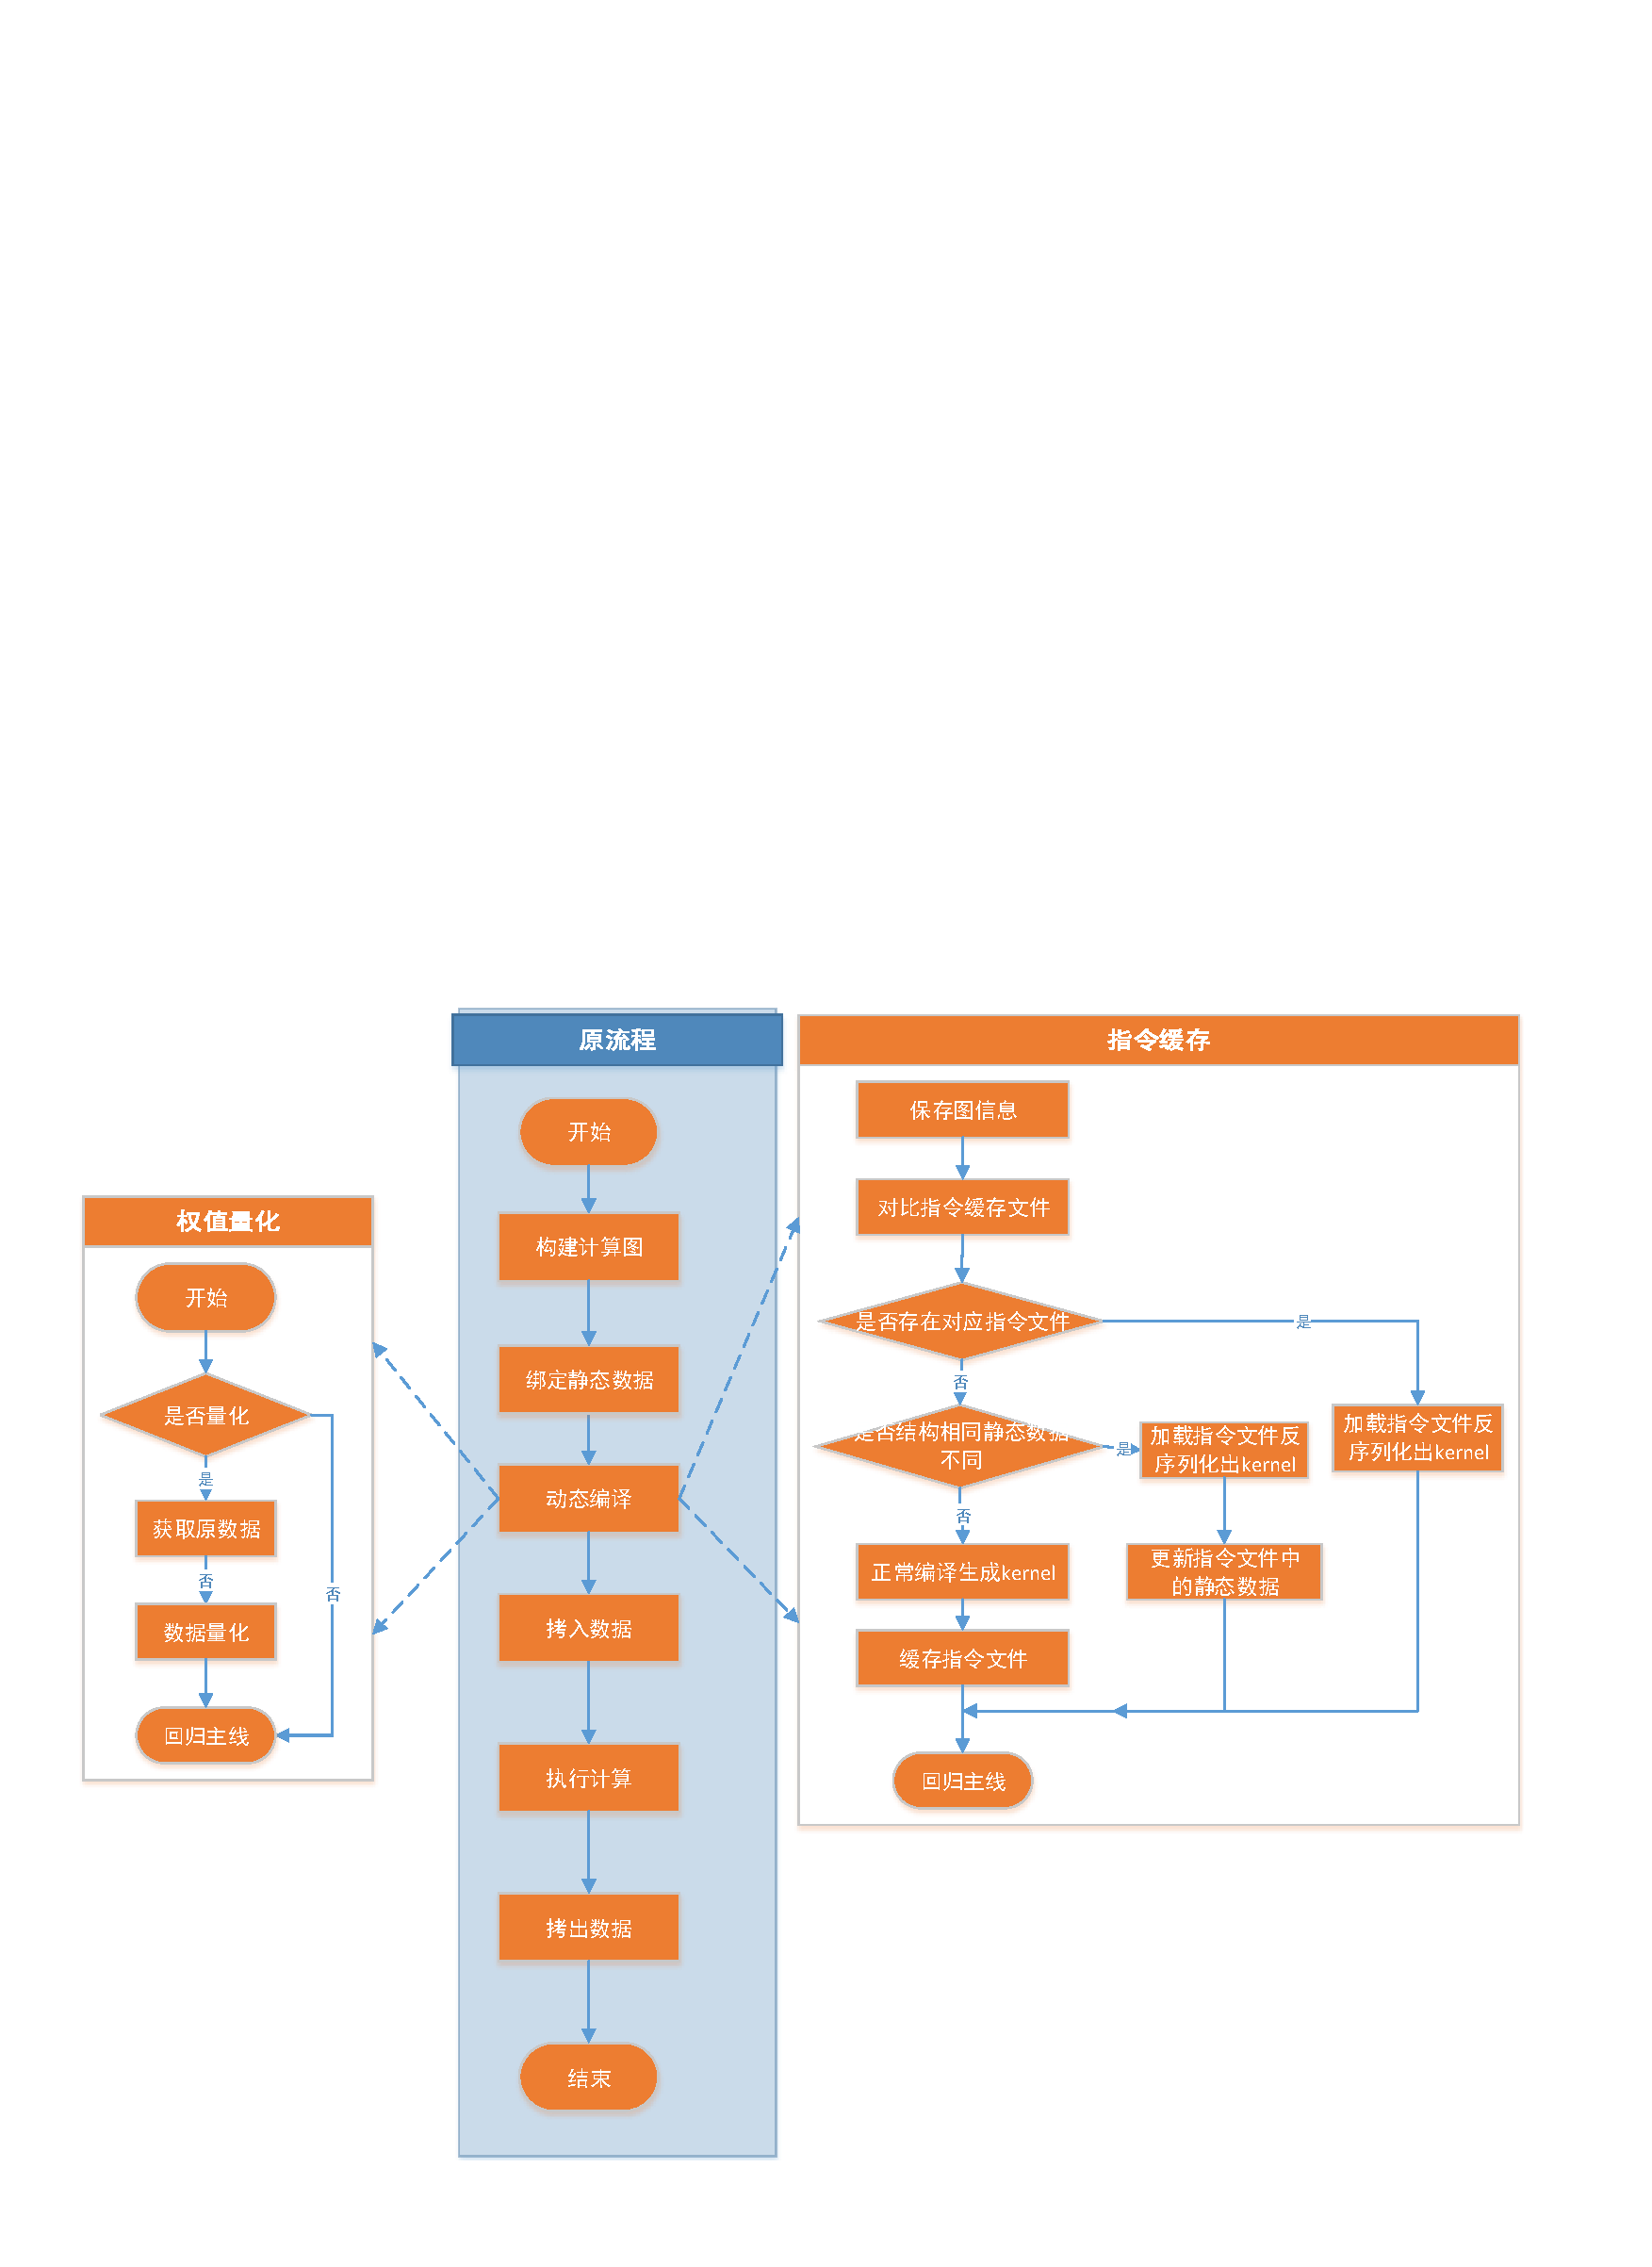
\includegraphics[width=0.8\textwidth]{main_process.pdf}
  \caption{运行时流程优化前后对比图}
  \label{fig:main-process}
\end{figure}

在动态编译过程中,引入权值量化。如果用户为了性能允许对权值等静态数据进行量化,则获取到原始用户传进来的数据,对原始数据进行精度量化,然后保存量化后的数据,节省网络的存储空间。

如果用户允许使用指令缓存功能,则在动态编译阶段,引入编译优化流程。在编译优化过程中,首先保存环境信息,环境信息包括硬件环境和软件环境,软件环境简可以直接用库版本信息表示。如果前后两次环境信息不一致,必须重新编译。其次是保存计算图信息,计算图信息也由两部分组成,第一个是用户传进来的神经网络的结构信息,保存神经网络的拓扑结构,第二部分是用户绑定的静态数据,静态数据包含权值和偏置值。如果结构信息和静态数据全和之前的一致,则可以直接加载以前缓存的指令,如果仅仅是静态数据变了,在更新静态数据后加载指令即可,如果结构信息和数据信息都不一致,则需要重新编译,并缓存这次编译好的指令作为备用。

\subsection {模块分解}
整个运行时优化可以分为三部分,编译优化,I/O优化和内存优化。针对每一个部分,都能做一定的优化措施,以便提升整体的运行流程。本系统主要从编译优化和内存优化的角度考虑。编译优化模块的主要目标是避免相同神经网络的重复编译,减少编译时间,节约编译资源;内存优化的主要目标是提升内存的利用率。为了实现编译优化和内存优化的目的,将主目标拆解,分为图信息识别模块、图信息保存模块、指令保存和加载模块、权值替换模块、指令替换模块、权值量化模块,模块分解如图~\ref{fig:model-split}所示。

\begin{figure}[htb]
  \centering
  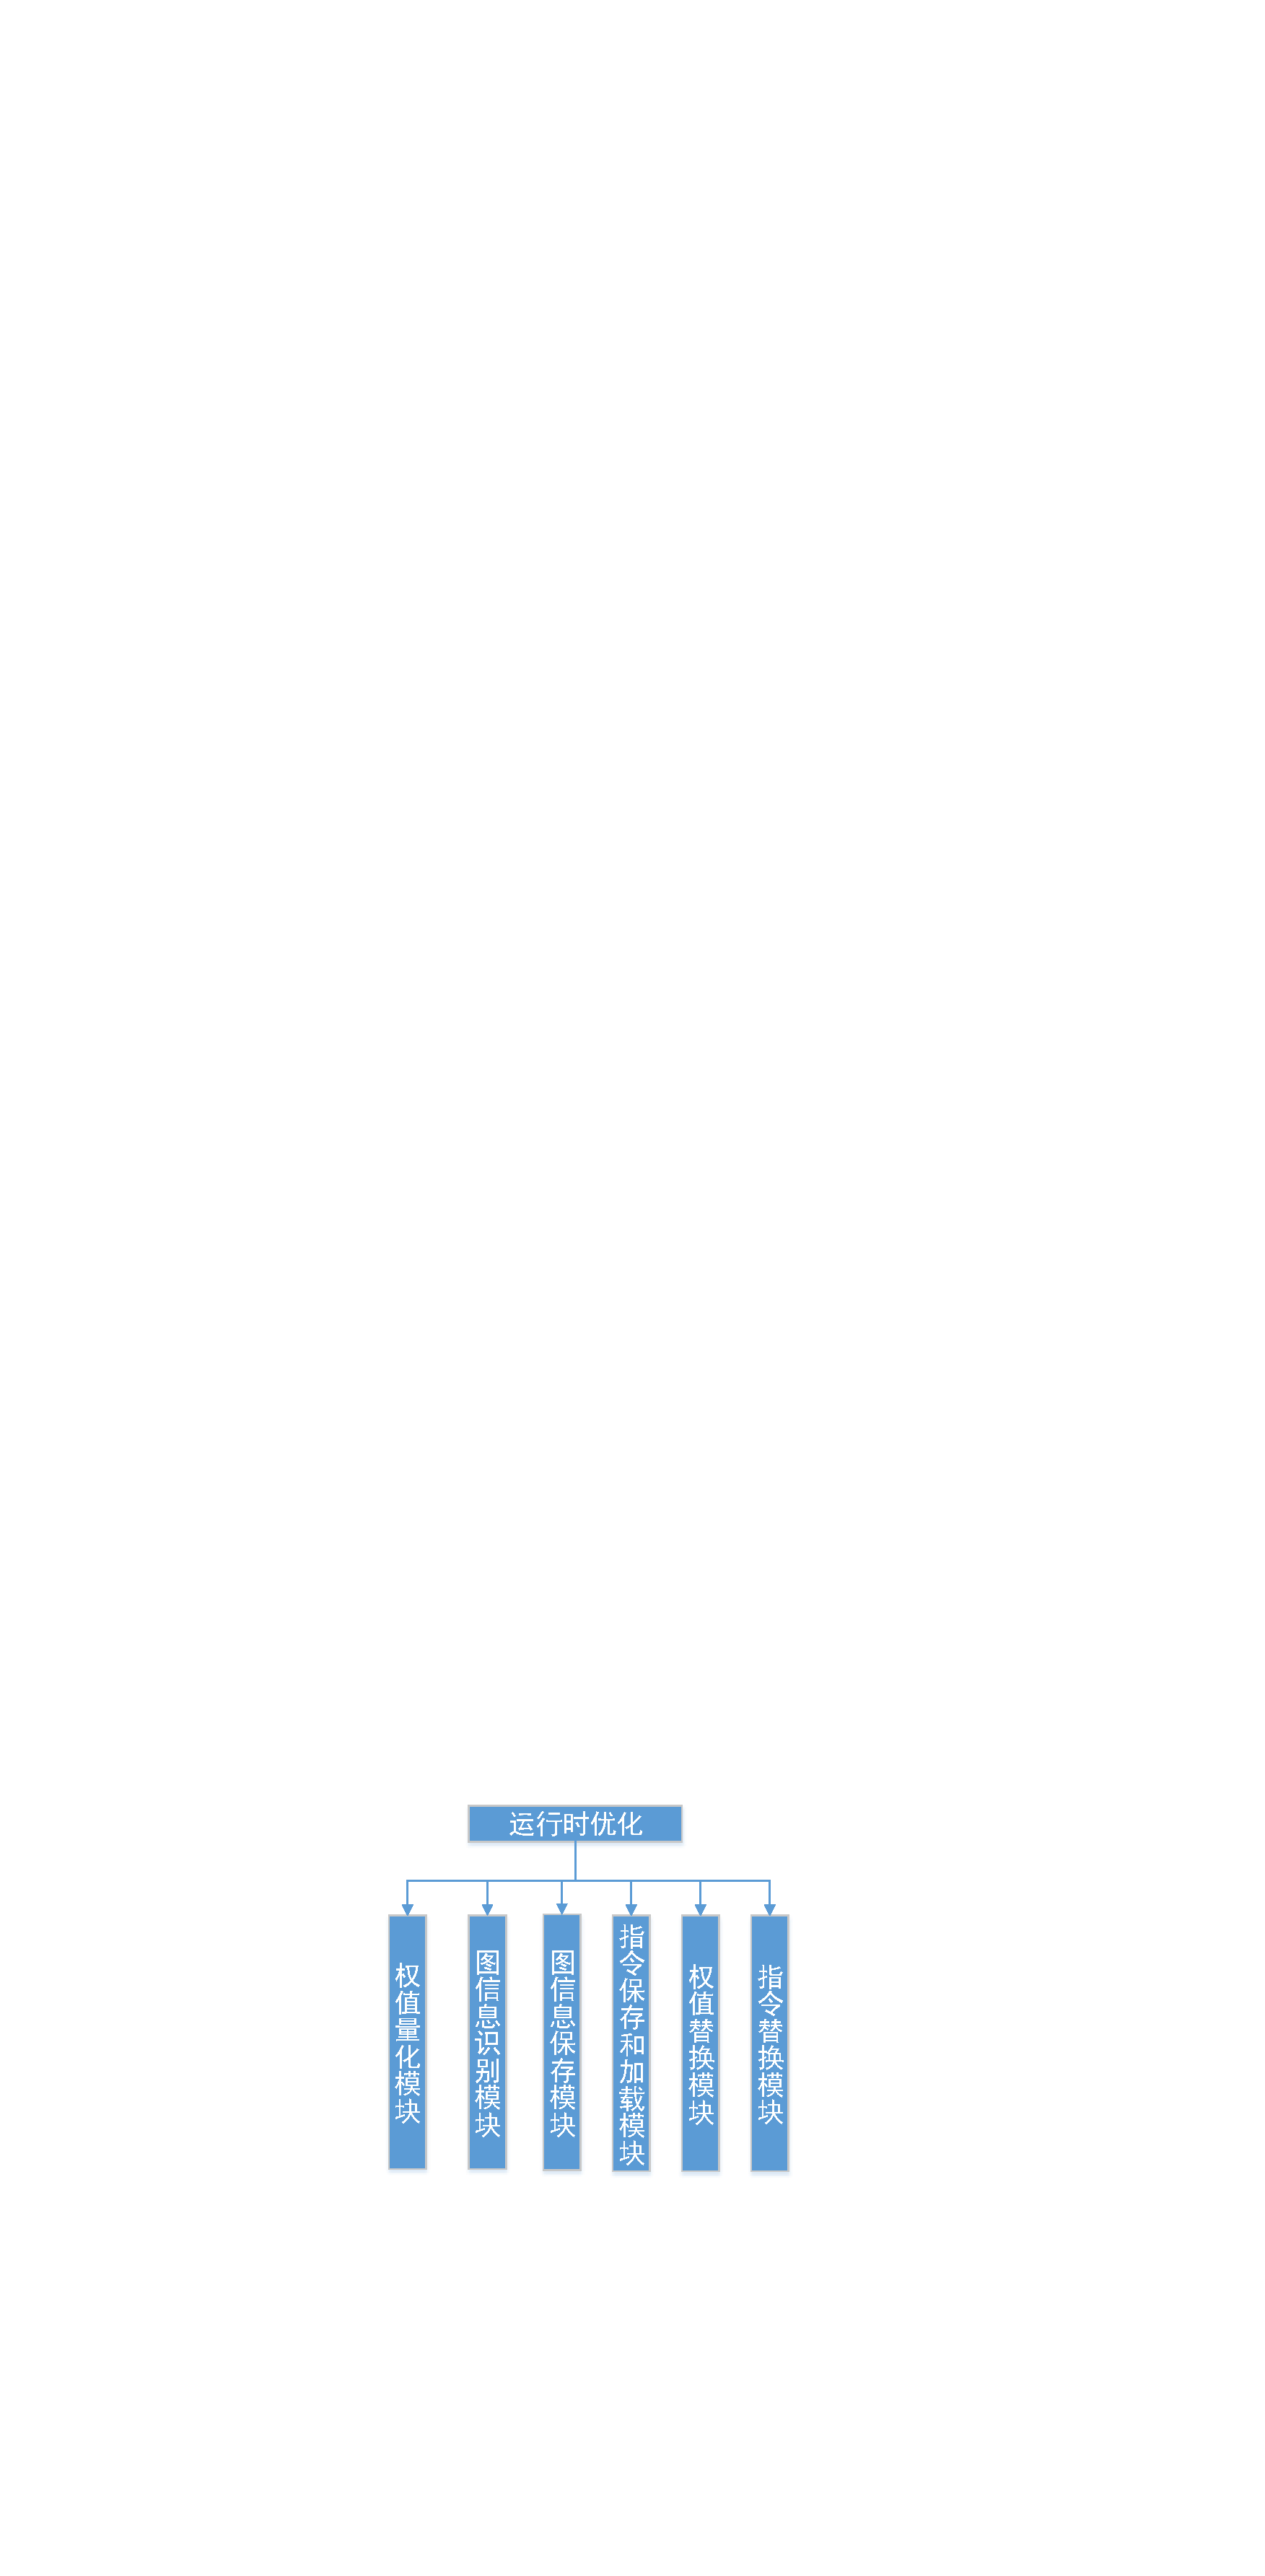
\includegraphics[width=0.6\textwidth]{model_split.pdf}
  \caption{模块分解图}
  \label{fig:model-split}
\end{figure}

\section {图信息保存模块}
\subsection {功能概述}
计算图信息保存模块是整个动态编译优化的基础,DNNCL库是声明式编程模式,用户所有的计算任务都存在计算图中。图信息保存模块的主要功能就是在编译的入口阶段,根据用户搭建的计算图,反向解析出用户的神经网络结构信息、权值信息以及运行环境等信息。

\subsection {设计思路}
一般而言,用户在框架层面可以利用神经网络模型文件构建计算图,但是DNNCL库是没办法直接拿到用户原始的网络模型文件的,并且不同框架的网络模型文件往往都不一样。例如caffe用prototxt文件保存结构信息,用caffemodel文件存储训练好的参数;TensorFlow用pb文件保存图的结构信息,用ckpt文件保存训练后的参数信息,还有一种pb和ckpt的结构体,同时保存结构信息和参数信息。

DNNCL库拿到的计算图信息抽象来看就是一个用户定义的操作(operation)数组,操作包含了计算的输入输出,计算细节,以及权值等信息,所以可以从用户构建的操作中反解析出原始的神经网络结构和权值信息。

为了方便起见,将计算图信息分为三部分:环境信息,结构信息和权值信息。环境信息包含了当前的软件版本已经底层的硬件型号,结构信息即为用户经网络的拓扑结构,权值信息即为神经网络的权值,是与输入数据无关的静态数据。三部分信息都用Json文件格式存储。Json采用键值对的方式来保存信息,是一种广泛使用的数据通信格式,具有轻量级,易阅读、修改和编写的特点,很适合用来保存我们所需要的信息。

\subsection {环境信息保存}
环境信息由一个包含4个键值的Json对象对保存,4个Key分别是:DNNCLversion, DNNCLrtversion,Driverversion,Hardwareversion,4个value的类型都是string。环境信息节点定义如表~\ref{tab:env-node}所示。

\begin{table}[htb]
  \centering\small
  \caption{环境信息组成表}
  \label{tab:env-node}
  \begin{tabular}{lclc}
    \toprule
    键        & 键类型    & 值    & 值类型                         \\
    \midrule
    DNNCLversion   & string  & DNNCL库版本       &string\\
    DNNCLrtversion & string  & DNNCL运行时库版本 &string\\
    Driverversion  & string  & 驱动版本          &string\\
    Hardwareversion & string  & 硬件型号 & string \\
    \bottomrule
  \end{tabular}
\end{table}

\subsection {权值信息保存}
权值信息代表神经网络的参数信息,包括权重和偏置值。如果用户声明的操作中绑定了静态数据,那么这部分数据就需要被保存下来。由于神经网络中权重的数据量很大,少则成千上万个,多则几十万、几百万个,如果每个都按原数值存储,可读性不强,需要的存储空间也很大。所以这里用信息摘要算法对权值数据进行处理,得到一个固定长度的信息摘要编码。如果信息摘要编码不一样,则代表原数据肯定不同。

权值信息由节点组成的Json数组表示,每个节点是一个Json对象。节点包含2个键值对,2个key分别是,name和staticdata;2个value的类型分别是string和Json对象组成的数组。节点的定义如表~\ref{tab:node-tab}所示。

\begin{table}[htb]
  \centering\small
  \caption{节点定义表}
  \label{tab:node-tab}
  \begin{tabular}{lcccl}
    \toprule
    键        & 键类型    & 值    & 值类型     &备注                    \\
    \midrule
    name   & string  & 节点名称 &string  &代表保存的数据属于哪个操作\\
    staticdata & string  & 数据信息 &string & Json对象数组 \\
    \bottomrule
  \end{tabular}
\end{table}

节点name唯一,是节点的唯一标识符,name表示这些数据属于哪一个操作。节点staticdata对应的值是一个Json数组,其元素是一个个Json对象,每个对象包含两个键值对,这两个键值对的两个键为key、value,两个值的类型都是string。这样设计staticdata是因为不同类型的操作绑定静态数据的情况可能不一样。例如某些算子包含多个输入,但是没有filter和bias,并且输入中一个或者多个绑定了静态数据;某些算子包含filter和bias,静态数据绑定在这些Tensor上。为了支持这些复杂的情况,采取了值为Json数组的设计方案。static data 定义如表~\ref{tab:data-tab}所示。

\begin{table}[htb]
  \centering\small
  \caption{static data 定义表}
  \label{tab:data-tab}
  \begin{tabular}{lcccl}
    \toprule
    键        & 键类型    & 值    & 值类型     &备注                    \\
    \midrule
    key   & string  & 属性名 &string  & Tensor的名称,是Tensor的唯一标识符\\
    value & string  & 属性值 &string & Tensor的数据信息摘要编码 \\
    \bottomrule
  \end{tabular}
\end{table}

\subsection {结构信息保存}
结构信息由节点组成的Json数组保存,每个节点是Json对象。节点分为两类,张量节点和操作节点。张量节点包含3个键值对,3个key分别是name、tensortype、datatype、datashape,4个value的类型都是string类型,张量节点的定义如图表~\ref{tab:struct-tab}所示。

\begin{table}[htb]
  \centering\small
  \caption{张量节点定义表}
  \label{tab:struct-tab}
  \begin{tabular}{lcccl}
    \toprule
    键        & 键类型    & 值    & 值类型     &备注       \\
    \midrule
    name   & string  & 节点名称 &string  & 不能有冒号\\
    tensorType & string  & 张量类型 &string & 已定义的枚举类型 \\
    attrs & string  & 张量属性 & Json数组 & 元素是Json对象 \\
    \bottomrule
  \end{tabular}
\end{table}

节点name唯一,是节点的唯一标识符,节点之间的连接关系,通过name进行索引,名字不能含有冒号。

节点tensortype代表数据节点的类型,有三种可选类型:Placeholder、Filter和Const。Placeholder代表这块数据是神经网络的输入,在运行时用户传入后才确定具体数值。Filter代表权重信息,在构建计算图的时候以及绑定具体的数据;Const表示静态类型数据,bias属于这一类。同Filter一样,也需要在构建计算图时绑定。

节点attrs对应的值是个Json对象数组,其设计方案和4.2.4节中datas节点相同,都包含两个键值对,键的名称为key和value,值的类型都为string。用来保存Tensor的数据类型和维度等基本信息。数据的存储类型,常用的有float32、float16、int8、int4。维度信息描述Tensor的形状,例如维度信息的值是:96、3、112、112。则代表数据有4个维度,可以看成是一个4维数组,第一个维度大小是96,第二个维度大小是3,第三个第四个维度都是112。

操作节点也由4个键值对组成,4个键分别是,name、optype、inputs、attrs,4个值的类型分别是string、string、string组成的Json数组、Json对象组成的Json数组。

节点name,操作节点的唯一标识符,功能和数据节点的name一样,用作图关系的索引。

节点optype,操作节点的类型,属于哪一类运算,常见的有conv、mlp、avtive、pool等。

节点inputs是由其它节点的name组成的数组,但前驱节点是包含多个输出的操作时,需要指明当前的输入是其前驱节点的哪个输出,用\$input\_name:\$num的方式指明这个信息。
节点attrs的定义和数据节点相同,只不过是保存的属性需要根据具体操作来定,有的多有的少。操作节点定义如表~\ref{tab:op-struct-tab}所示。

\begin{table}[htb]
  \centering\footnotesize
  \caption{操作节点定义表}
  \label{tab:op-struct-tab}
  \begin{tabular}{lclll}
    \toprule
    键        & 键类型    & 值    & 值类型     &备注       \\
    \midrule
    name   & string  & 节点名称 &string  & 不能有冒号\\
    optype & string  & 操作类型 &string & 已支持的操作类型 \\
    attrs  & string  & 其它属性 & Json数组 & 由Json对象组成 \\
    inputs & string  & 输入节点名称 & Json数组 & 元素是字符串,用\$input\_name:\$num \\
                                          &&&&区分输入节点有多输出的情况 \\
    
    \bottomrule
  \end{tabular}
\end{table}

\subsection {接口设计}
该模块对外接口的主要接口及其功能如表~\ref{tab:env-interface-tab}所示。

\begin{table}[htb]
  \centering\footnotesize
  \caption{图信息保存模块对外接口}
  \label{tab:env-interface-tab}
  \begin{tabular}{ll}
    \toprule
    函数名       & saveEnvInfoToJson   \\
    \midrule
    输入 & 当前软件版本和硬件型号 \\
    输出 & 保存环境信息的Json对象  \\
    功能 & 保存环境信息\\
    说明 & 因为该部分信息与整个系统有关,不依赖与某个具体的操作,所以其实现应该独立于操作 \\
    \bottomrule
    \toprule
    函数名       & saveGraphInfoToJson    \\
    \midrule
    输入 & 操作 \\
    输出 & 保存操作结构信息的Json对象  \\
    功能 & 保存操作的结构信息\\
    说明 & 因为每个操作都有自己的结构,所以该方法定义成虚函数放在操作的基类中,\\
          &每个实现自己的逻辑 \\
    \bottomrule
    \toprule
    函数名       & saveDataInfoToJson    \\
    \midrule
    输入 & 操作 \\
    输出 & 保存操作静态数据信息的Json对象  \\
    功能 & 保存操作的静态数据信息\\
    说明 & 静态数据信息都绑定在对应的tensor上,根据tensor可以找到其绑定的数据信息\\
    \bottomrule
  \end{tabular}
\end{table}


\section {图信息识别模块}

\subsection {功能概述} 
图信息识别模块是在图信息已经被保存的基础上比较当前的图信息在近期是否已经编译过,如果编译过,则直接加载缓存的指令,避免重复编译。

\subsection {设计思路}
在4.3节中,我们所需的三部分信息都保存为Json格式的文件,最简单的方式就是分别对两个文件进行字符串检查,如果内容完全一样,则代表保存的信息相同。这样思路简单,但是有很多不好地方: 
\begin{enumerate}
  \item 如果比较文件内容,则不仅需要缓存指令文件还需要缓存图信息文件,需要更多的存储空间
  \item 对文件内容进行比较较为麻烦,需要拿当前保存的文件与之前所有缓存的文件进行对比
\end{enumerate}

所有决定采用储存信息表的方式。首先利用信息摘要算法对三个文件进行处理,根据文件内容生成一个唯一的信息摘要编码,然后建立三张信息表:环境信息表、结构信息表、权值信息表。环境信息表缓存环境信息摘要编码,结构信息表缓存结构信息摘要编码,权值信息缓存数据信息编码,信息表的结构如表~\ref{tab:info-tab}所示。

\begin{table}[htb]
  \centering\small
  \caption{信息表结构}
  \label{tab:info-tab}
  \begin{tabular}{c}
    \hline
    摘要编码1    \\ \hline
    摘要编码2    \\ \hline
    摘要编码3    \\ \hline
    ...         \\ \hline
  \end{tabular}
\end{table}

\subsection {接口设计}
该模块对外接口的主要接口及其功能如表~\ref{tab:info-interface-tab}所示。

\begin{table}[htb]
  \centering\small
  \caption{图信息识别模块对外接口}
  \label{tab:info-interface-tab}
  \resizebox{\textwidth}{72mm}{
  \begin{tabular}{ll}
    \toprule
    函数名       & generateSummaryCode   \\
    \midrule
    输入 & 一个字符串 \\
    输出 & 该字符串对应的信息摘要编码  \\
    功能 & 生成信息摘要编码\\
    说明 & 根据输入字符串的内容,利用信息摘要算法,生成唯一的固定长度的唯一编码 \\
    \bottomrule
    \toprule
    函数名       & saveCodeToCacheTable    \\
    \midrule
    输入 & 两个输入,一个是要打开的文件名,一个是要写入文件的信息摘要编码 \\
    输出 & 内容更新后的文件  \\
    功能 & 将信息摘要编码保存到文件中\\
    说明 & 新内容要写入到文件头,存储的编码达到数量限制时应该删除末尾的内容 \\
    \bottomrule
    \toprule
    函数名       & findCodeInCacheTable \\
    \midrule
    输入 & 两个输入,一个是文件名, 一个是需要查找的信息摘要编码 \\
    输出 & 布尔值,表示信息摘要编码是否存在文件中  \\
    功能 & 在指定的文件中国查找指定的信息摘要编码 \\
    说明 & 从前往后查找, \\
    \bottomrule
    \toprule
    函数名       & getCacheModelName \\
    \midrule
    输入 & 三个信息摘要编码 \\
    输出 & 匹配的缓存指令的文件名  \\
    功能 & 判断当前缓存区中是否有符合要求的指令缓存文件 \\
    说明 & 如果找到返回缓存指令文件名,没找到返回空字符串\\
    \bottomrule
  \end{tabular}}
\end{table}

\section {指令保存和加载模块}

\subsection {功能概述}
该模块的主要目标是实现指令的离线保存和运行时加载,允许用户在编译之后离线保存编译后生成的指令,在需要使用的时候从文件中加载指令,然后结合当前的输入数据,完成神经网络的计算过程。

\subsection {通用深度学习模型设计}
在第二章的介绍中我们知道操作(operation)是对抽象操作(如 matmul 或者 add)的一个统称,而内核(kernel)则是能够运行在特定设备上的一种对操作的实现,可以将kernel看成是一种通用深度学习模型。如果把任意深度学习任务看成一个黑盒,那么除输入数据和输出结果外,其余所有在执行时所必需的数据称为通用深度学习模型,而这些数据都保存在kernel中。

在多核平台中,根据数据是否核间共享,可以将通用深度学习模型内的数据分为栈数据和堆数据。相应的,内存空间也分为栈区和堆区,每个核私有的栈数据存在栈区(一个核对应一个栈区),核间共享的堆数据存在堆区。根据在运行阶段数据是否可变,将堆数据分为静态数据和动态数据,注意栈数据都是静态数据。
栈数据(核内私有)包括中间结果的临时空间及其属性(大小、数据类型等),不可共享的网络模型数据(例如权值、偏置、均值、方差等)。

堆数据(核间共享):1)静态数据(在运行阶段不需要变)包括:机器指令、可共享的网络模型数据,硬件平台信息、硬件所需的专用参数集;2)动态数据(在运行阶段可变)包括:输入输出数据及其属性(大小、数据类型、规模等)。

一个典型的通用机器学习模型在内存中的布局如图~\ref{fig:general-model}所示。

\begin{figure}[htb]
  \centering
  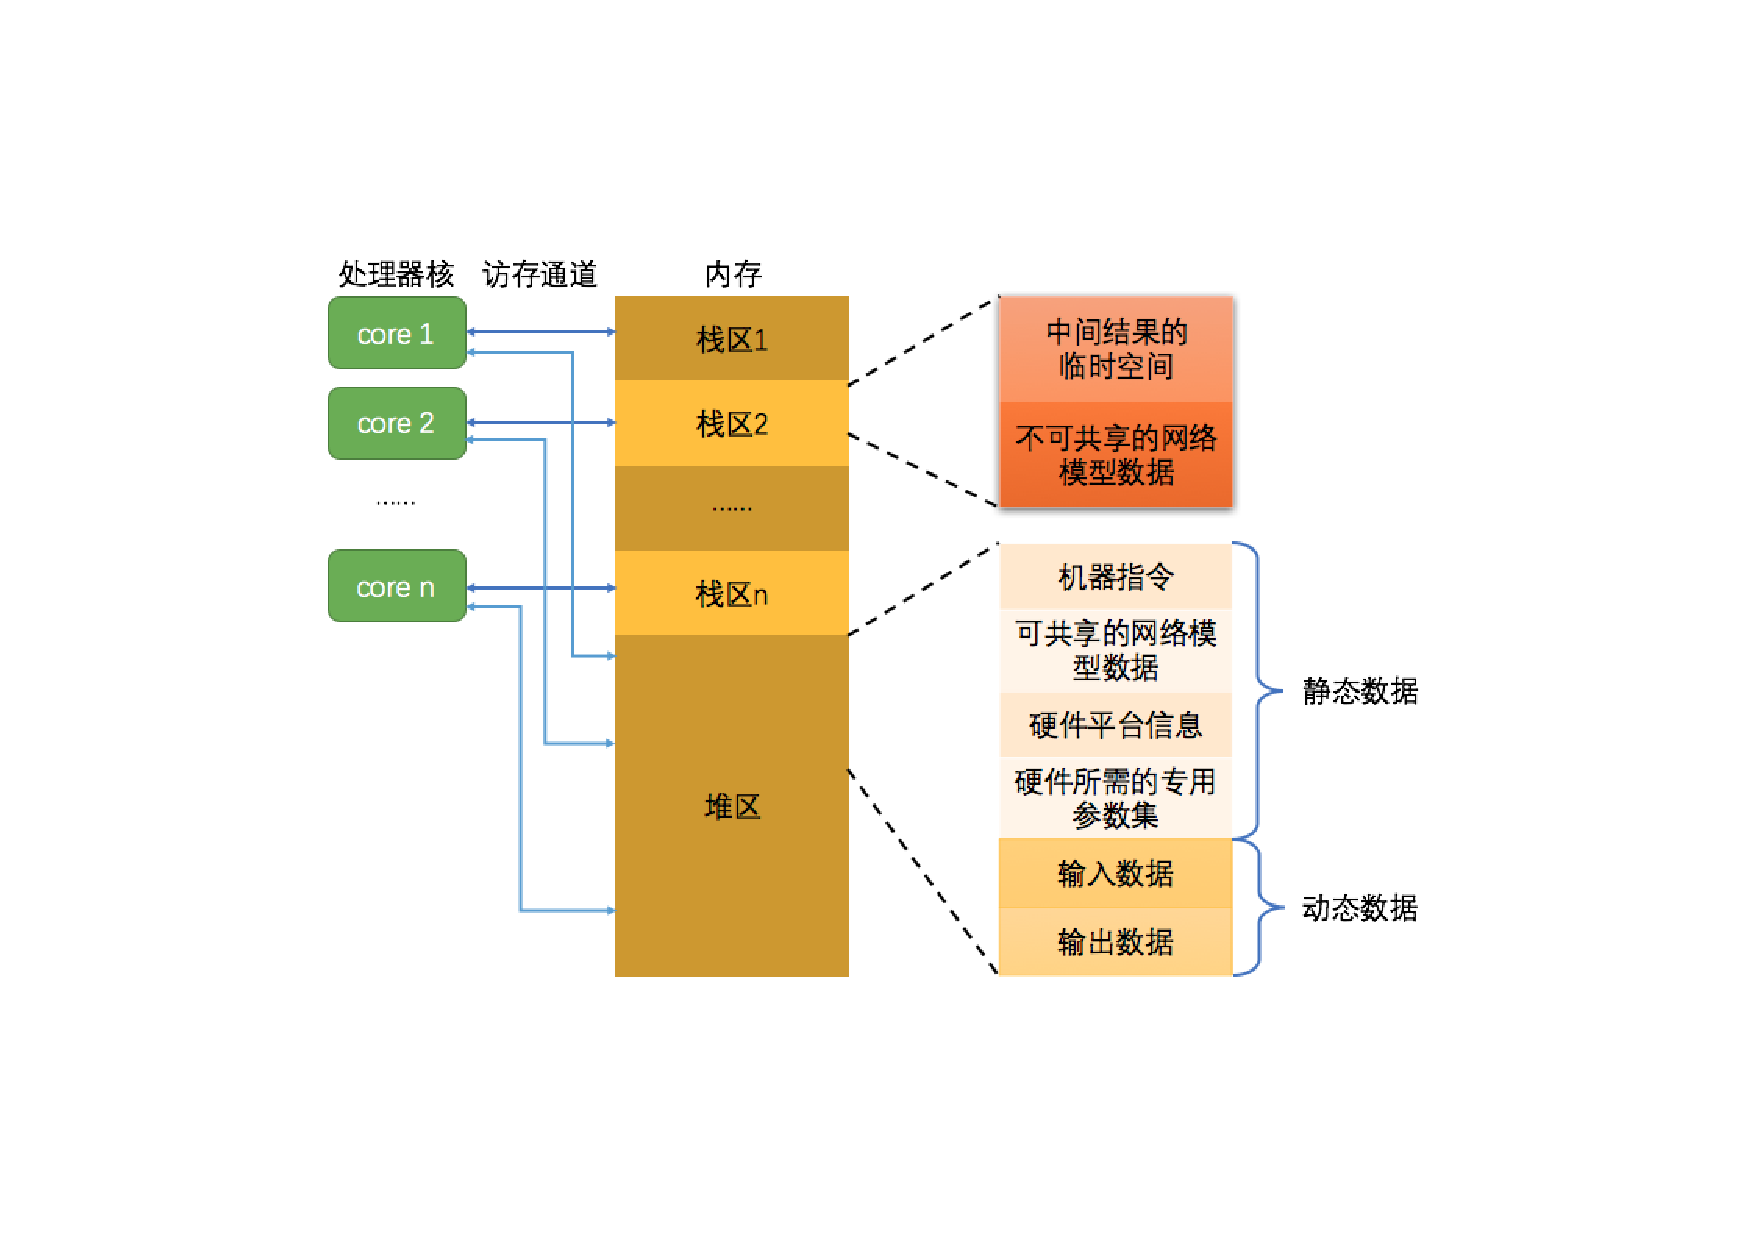
\includegraphics[width=0.6\textwidth]{general_model.pdf}
  \caption{机器学习内存布局图}
  \label{fig:general-model}
\end{figure}

生成通用深度学习模型的装置称为模型生成器(生成kernel),组成模块如图~\ref{fig:kernel-model}所示。
\begin{figure}[htb]
  \centering
  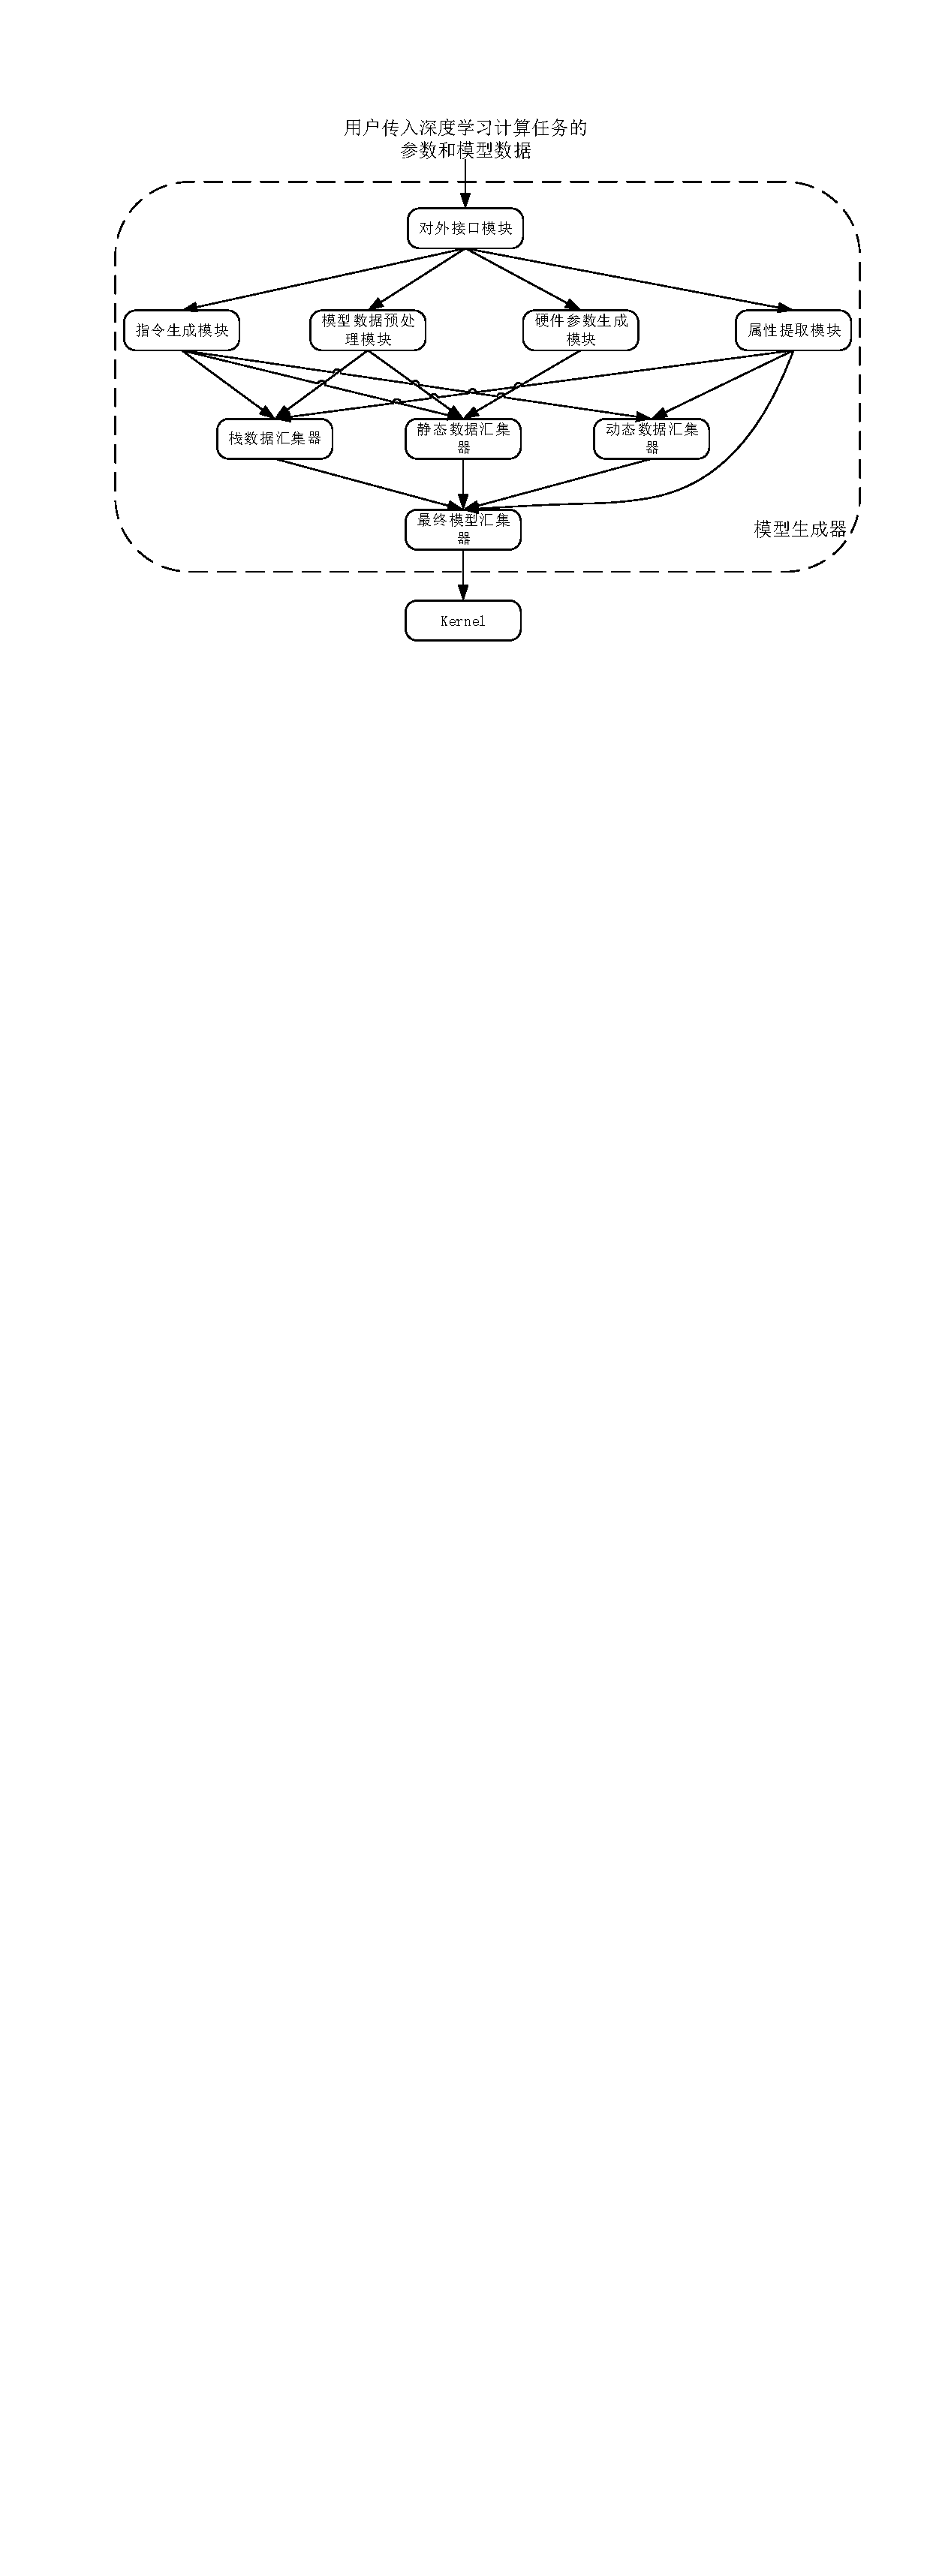
\includegraphics[width=0.8\textwidth]{kernel_model.pdf}
  \caption{kernel模块组成图}
  \label{fig:kernel-model}
\end{figure}

生成模型的步骤:
\begin{enumerate}
\item 对外接口模块接收用户传入的机器学习计算任务的参数和模型数据,将任务的参数和模型数据转换为对算法的描述信息(任务参数是用户传入的,所以不会销毁,也就是说存档),传递给指令生成模块、模型数据预处理模块、硬件参数生成模块;再将任务的参数传递给属性提取模块。
\item 指令生成模块根据算法描述信息编译生成二进制的机器指令,传递给静态数据汇集器;再计算出最佳的数据块布局传递给栈数据汇集器、静态数据汇集器、动态数据汇集器。
\item 模型数据预处理模块根据算法描述信息将机器学习模型数据做格式转换、拆分和分类,将不可共享的模型数据传递给栈数据汇集器,将共享模型数据传递给静态数据汇集器。
\item 硬件参数生成模块根据算法描述信息制造出硬件所需的专用参数集;再调用驱动程序的接口,获取硬件平台信息;然后将两者传递给静态数据汇集器。
\item 属性提取模块在机器学习计算任务的参数中提取出输入、输出数据、中间结果临时空间的属性,传递给最终模型汇集器;再从属性中提取出输入、输出数据的大小,创建各自的存储空间,传递给动态数据汇集器;再从属性中提取中间结果临时空间的大小,创建各自的存储空间,传递给栈数据汇集器。
\item 栈数据汇集器,将不可共享的模型数据和中间结果临时存储空间,根据数据块布局信息,打包整理成多段栈数据,传递给最终模型汇集器。
\item 静态数据汇集器,将机器指令、共享模型数据、硬件平台信息、硬件所需的专用参数集,根据数据块布局信息,打包整理成一段连续的静态数据,传递给最终模型汇集器。
\item 动态数据汇集器,将输入输出数据的存储空间,根据数据块布局信息,打包整理成一段连续的动态数据,传递给最终模型汇集器。
\item 最终模型汇集器,将输入输出数据和中间结果临时空间的属性、多段栈数据、连续的静态数据、连续的动态数据,合并成为一个核函数,保存在内存中。
\end{enumerate}

执行通用机器学习模型的装置模型执行器(运行核函数),其组成模块如图~\ref{fig:model-run}所示。
\begin{figure}[htb]
  \centering
  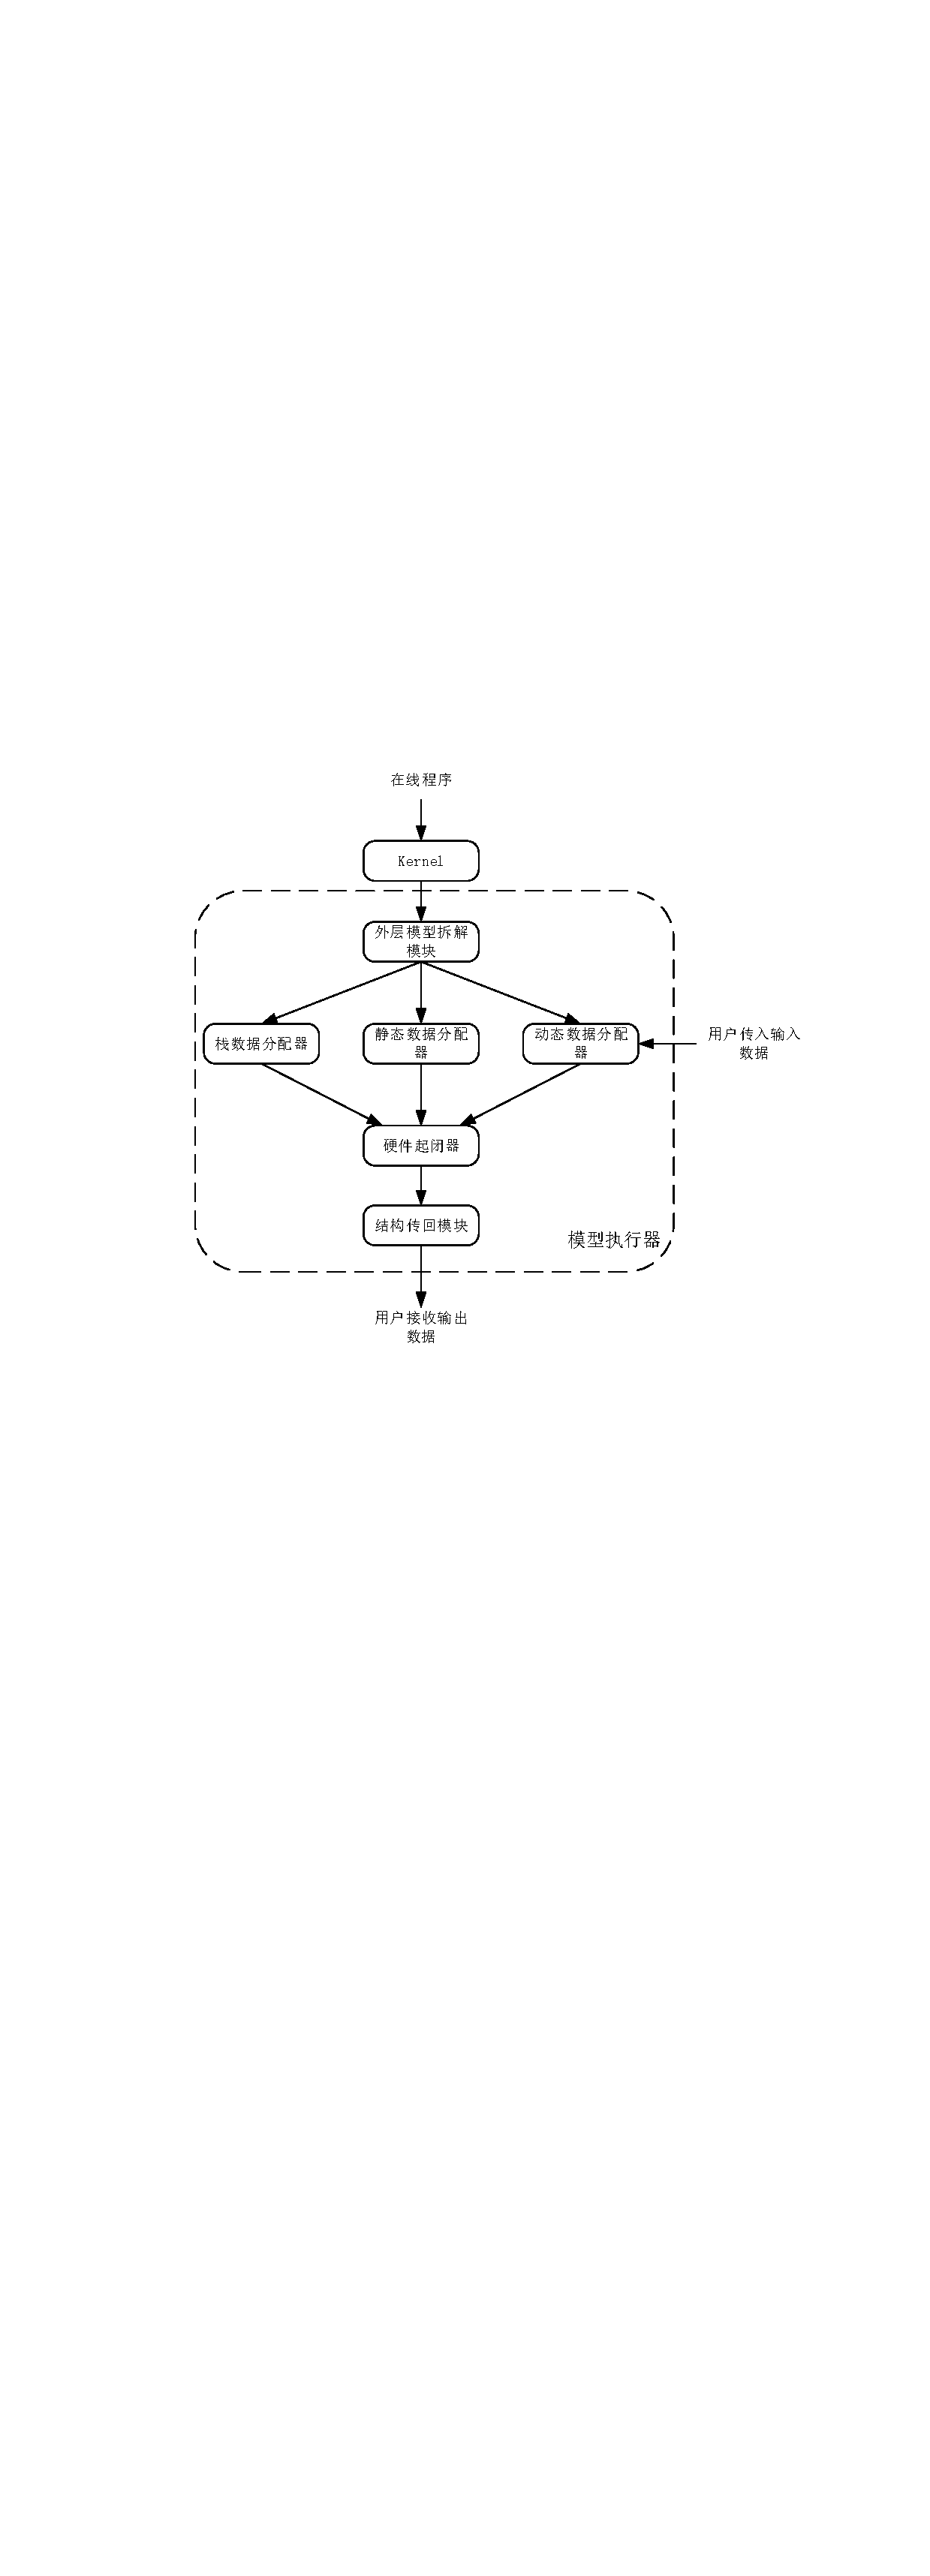
\includegraphics[width=0.6\textwidth]{model_run.pdf}
  \caption{模型执行器}
  \label{fig:model-run}
\end{figure}

执行流程:
\begin{enumerate}
\item 模型解析器读取磁盘上的离线文件,还原成内存中的核函数,传递给模型执行器。
以上步骤属于模型解析器的功能,以下步骤是模型执行器的功能。
\item 外层模型拆解模块,接收用户在线程序输入的或模型解析器给出的核函数;在其中取出输入、输出数据的属性,和一段动态数据,传递给动态数据分配器;取出中间结果临时空间的属性、多段栈数据,传递给栈数据分配器;取出静态数据,传递给静态数据分配器。
\item 栈数据分配器,在中间结果临时空间的属性中获取临时空间大小,加上每段栈数据的大小,计算出内存每个栈区需要占用的空间大小,并调用驱动程序,在各个栈区申请空间;再将每段栈数据拷入对应的栈区。
\item 静态数据分配器,根据静态数据的大小,调用驱动程序,在内存的堆区申请一块连续空间;再将静态数据拷入堆区。
\item 动态数据分配器,在输入、输出数据的属性中获取输入、输出数据大小,调用驱动程序,在内存的堆区申请多块空间(因为有可能多输入、多输出);再接收用户传入的输入数据,将它们拷入相应的堆区位置。
\item 硬件启闭器,调用驱动程序,启动硬件计算单元,开始计算;等待计算完成。
\item 结果回传模块,将输出数据从堆区取出,返回给用户。
\end{enumerate}

\subsection {指令缓存设计思路}
从上一节的介绍可以看出,kernel中保存了在设备上实现操作所需要的所有信息,想要实现指令缓存,最简单的方法就是实现kernel的离线保存和加载。所以我们可以实现一个模型保存器和一个模型解析器。模型保存器用来将多个kernel有序组织成一个离线文件,保存到磁盘中;模型解析器,用于将离线文件中的内容,还原成内存中的核函数,传递给模型执行器。

如图~\ref{fig:ins-cache-process}所示,在模型生成器生成kernel之后,利用模型保存器,将kernel保存到离线文件中。相应的,在模型执行器之前增加一个模型解析器,用于从离线文件中解析出kernel。

\begin{figure}[htb]
  \centering
  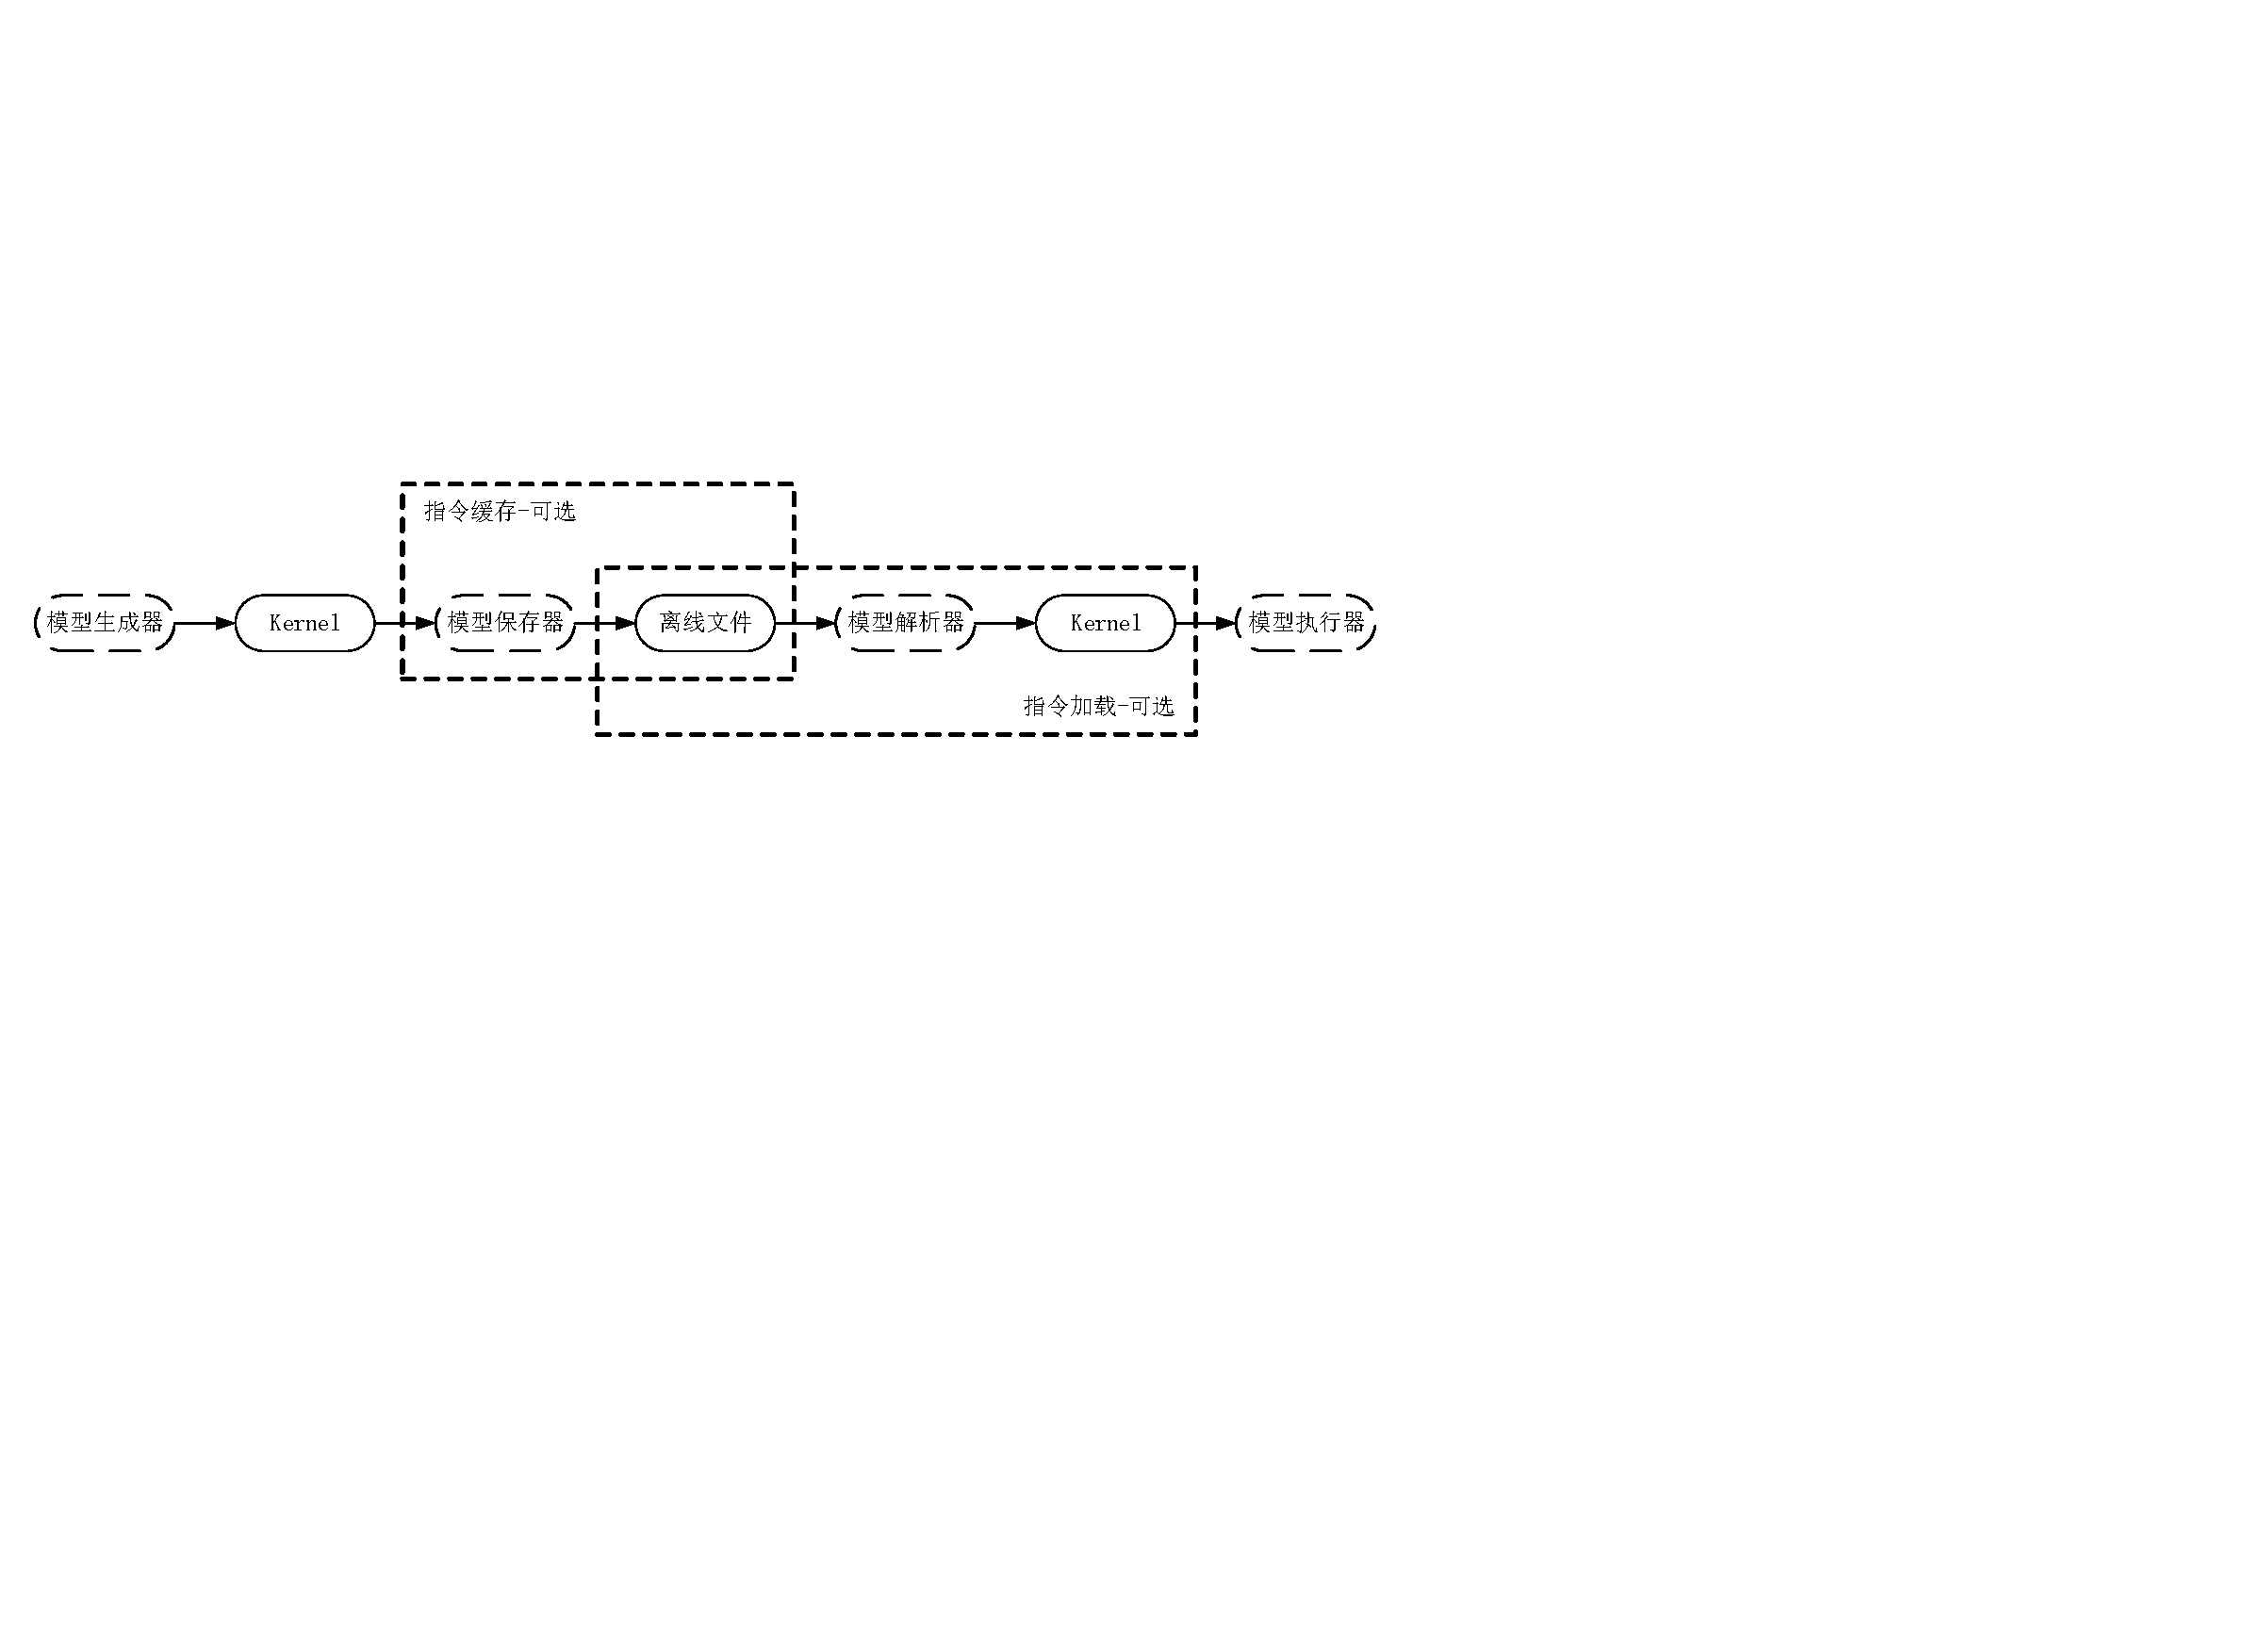
\includegraphics[width=1.0\textwidth]{ins_cache_process.pdf}
  \caption{指令缓存处理流程}
  \label{fig:ins-cache-process}
\end{figure}

所以离线模型文件是本模块的基础,离线模型文件的结构决定了模型保存器和模型生成器的处理流程,离线模型文件的结构设计如图~\ref{fig:offline-model-struct}所示。

\begin{figure}[htb]
  \centering
  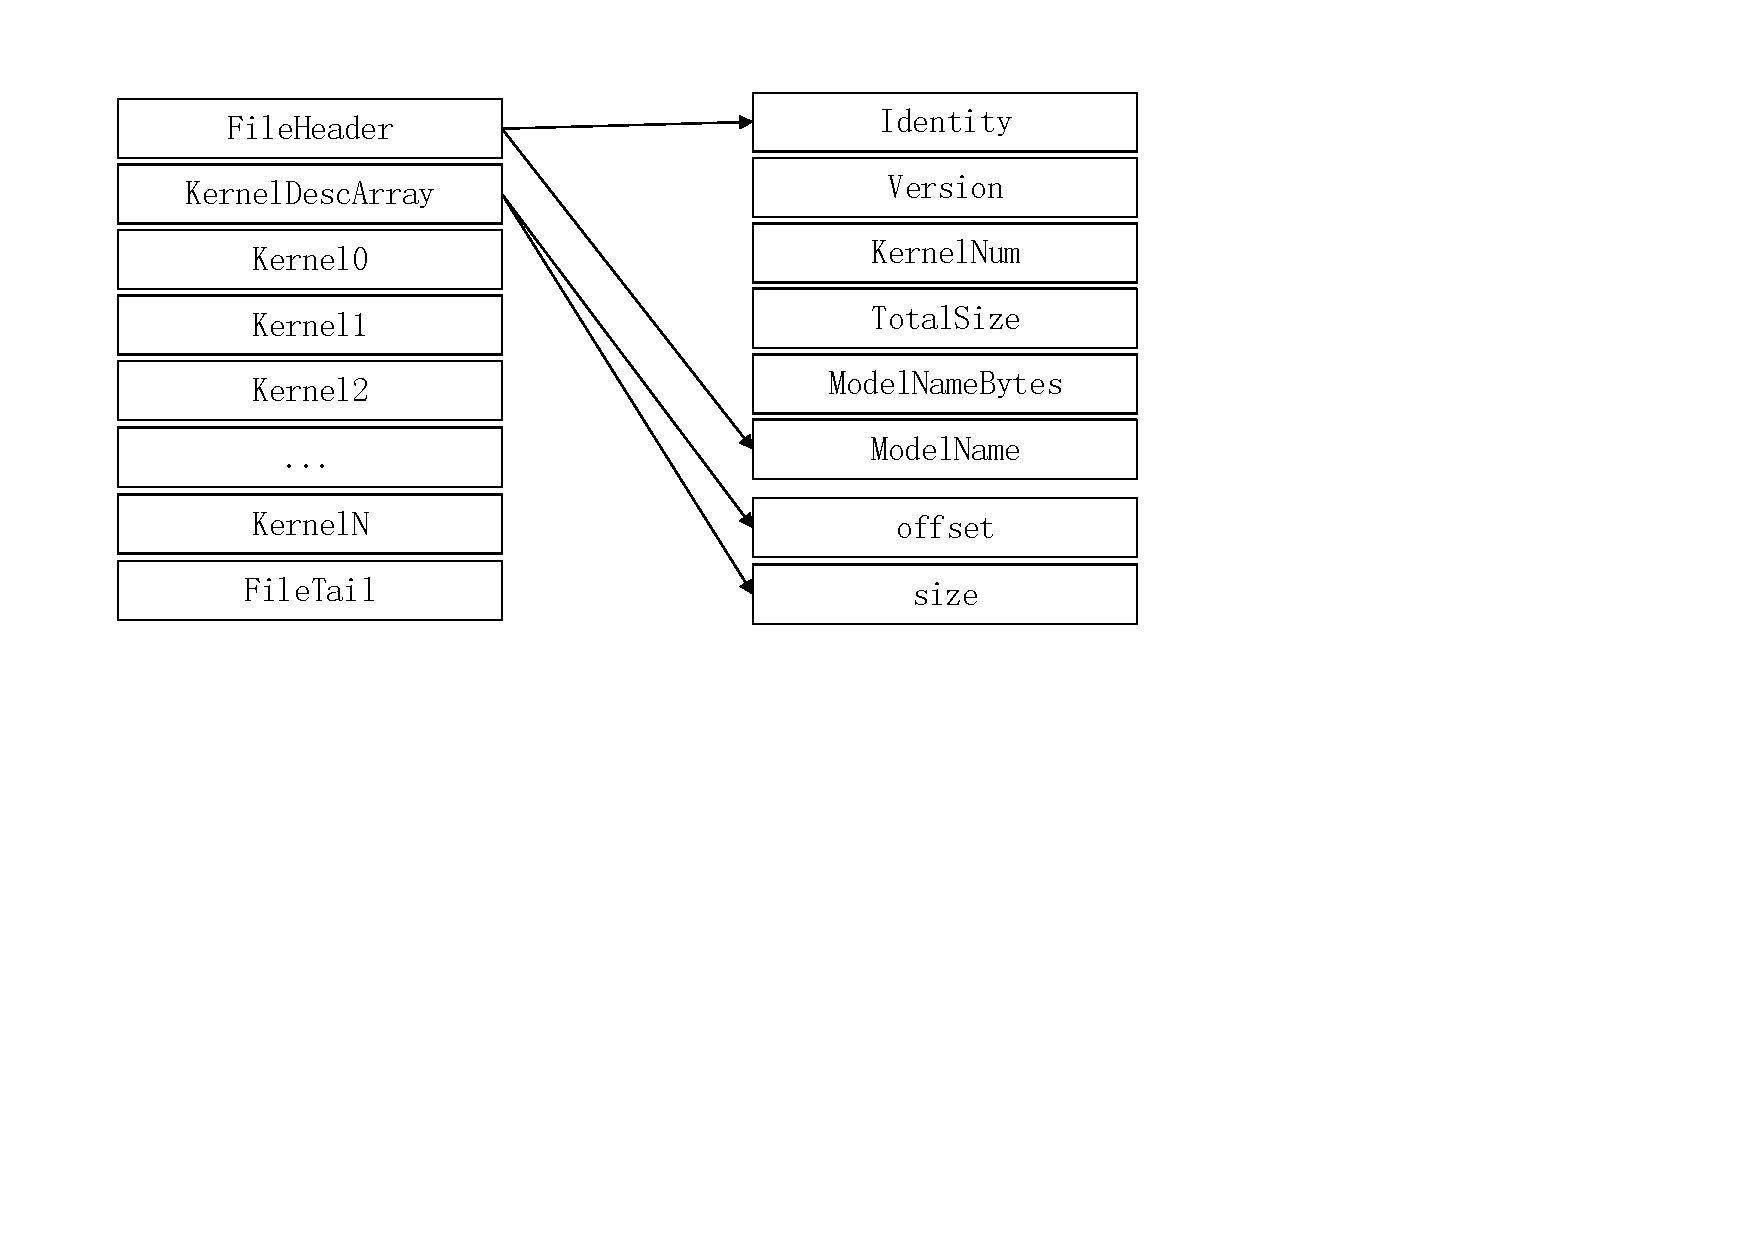
\includegraphics[width=0.6\textwidth]{offline_model_struct.pdf}
  \caption{离线模型结构}
  \label{fig:offline-model-struct}
\end{figure}

离线模型文件包含4部分:文件头,目录,具体内容,文件尾。最开始是固定大小的文件头;然后是一个数组,数据元素是kernel的描述信息,相当于文件内容的目录;紧接着是具体的kernel,保存kernel的详细信息;最后是文件尾。文件头和文件尾用于文件判别和校验,防止存储和传输图中文件的损坏;文件目录用于读取kernel的详细内容。 
文件头各部分的定义如表~\ref{tab:file-header}所示。为了解析文件的方便,FileHeader大小,为1024字节即1k,前4部分固定大小为4字节,最后用1008字节存储模型名称,空位补零填充。

\begin{table}[htb]
  \centering\small
  \caption{FileHeader结构定义}
  \label{tab:file-header}
  \begin{tabular}{llll}
    \toprule
    名称          & 类型     & 大小(字节)   & 备注       \\
    \midrule
    Identity      & string  & 4    & 文件类型检验码  \\
    Version       & string  & 4    & 离线模型版本 \\
    KernelNum     & uint64  & 4    & 文件里包含多少个kernel  \\
    TotalSize     & uint64  & 4    & 文件总大小  \\
    ModelNameBytes& uint64  & 4    & 模型名称占用多少字节  \\
    ModelName     & string  & 1008 & 模型名称  \\
    \bottomrule
  \end{tabular}
\end{table}

KernelDescArray是文件目录,实际是一个数组,数组元素是KernelDesc,数组大小和文件中保存的Kernel数量相同。KernelDesc只有两个字段:offset和size。offset当前kernel的存储位置相对于文件起始的偏移量,size表示当前kernel内容的大小。KernelDescArray可以类比于书本的目录,根据目录可以找到对应章节在哪一页,同样读文件时可以根据KernelDescArray中kernel的大小和偏移来读取指定kernel的内容。KernelDesc的定义如表~\ref{tab:kernel-desc}所示。

\begin{table}[htb]
  \centering\small
  \caption{kernelDesc定义}
  \label{tab:kernel-desc}
  \begin{tabular}{lccl}
    \toprule
    名称      & 类型     & 大小(字节)   & 备注       \\
    \midrule
    offset    & uint64  & 4    & 相对于文件头的偏移  \\
    size      & uint64  & 4    & kernel的大小 \\
    \bottomrule
  \end{tabular}
\end{table}

离线模型文件中Kernel的内容可以看作是kernel结构经过压缩和加密算法处理,序列化后生成的字符串。

FileTail中只含有一个字段,用来存储校验码,校验码的内容是根据本文件中除文件尾以外的所有内容生成的一个信息摘要编码,如表~\ref{tab:file-tail}所示。

\begin{table}[htb]
  \centering\small
  \caption{FileTail定义}
  \label{tab:file-tail}
  \begin{tabular}{lccl}
    \toprule
    名称      & 类型     & 大小(字节)   & 备注       \\
    \midrule
    CheckCode & string  & 16   & 长度为16个字符的MD5码  \\
    \bottomrule
  \end{tabular}
\end{table}

根据离线模型的定义,我们知道模型保存器应该具有模型压缩加密、计算文件大小、填充文件头、填充目录、填充kernel、填充文件尾等功能。模型保存器的组成如图~\ref{fig:mode-save}所示。

\begin{figure}[htb]
  \centering
  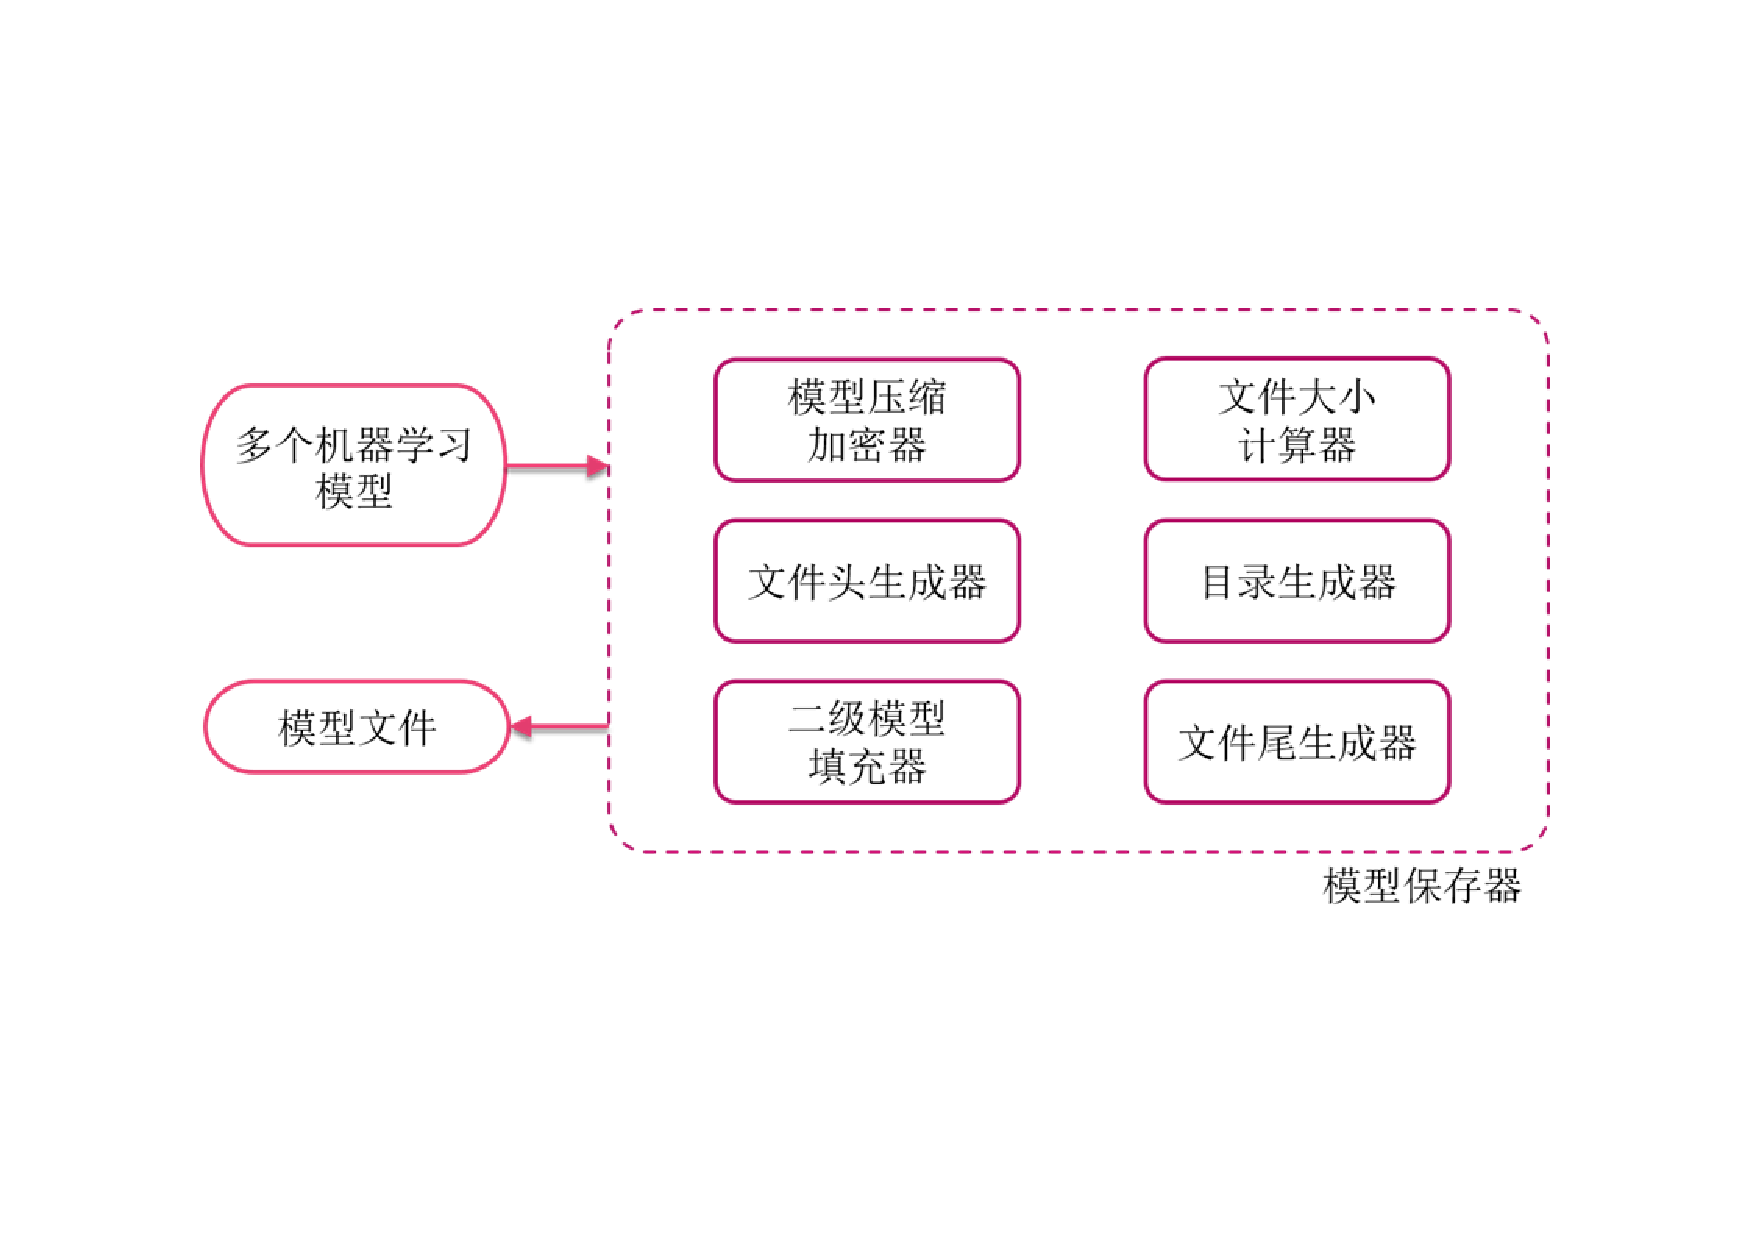
\includegraphics[width=0.8\textwidth]{model_save.pdf}
  \caption{模型保存器}
  \label{fig:mode-save}
\end{figure}

各部分的功能如下:
\begin{itemize}
  \item 模型压缩加密器用于接收多个机器学习模型,按一定压缩和加密算法对他们进行压缩和加密,得到二级模型(序列化后的字符串);
  \item 二级模型填充器用于计算每个二级模型占用存储空间的大小和模型总数量,将二级模型写入模型文件;
  \item 文件大小计算器用于接收二级模型占用存储空间的大小和模型数量,计算所有二级模型所需总大小,计算二级模型目录占用存储空间大小,加上文件头和文件尾大小,计算出模型文件总大小;
  \item 文件头生成器用于接收模型文件总大小和模型数量,产生模型文件标识码(用于区分本文件格式与其他文件不同),写入模型文件;
  \item 目录生成器用于接收二级模型占用存储空间的大小和模型数量,计算每个模型在文件中的偏移量,形成目录表,写入模型文件;
  \item 文件尾生成器将模型文件前面已写完的部分按一定算法计算校验码,写入模型文件最后,用于防止传输图中出错;
\end{itemize}

模型解析器要按照设计好的格式读取离线模型文件并解析出kernel,所以模型解析器应该具有文件校验、目录解析、模型解析等功能。模型解析器的组成如图~\ref{fig:model_praser}所示。

\begin{figure}[htb]
  \centering
  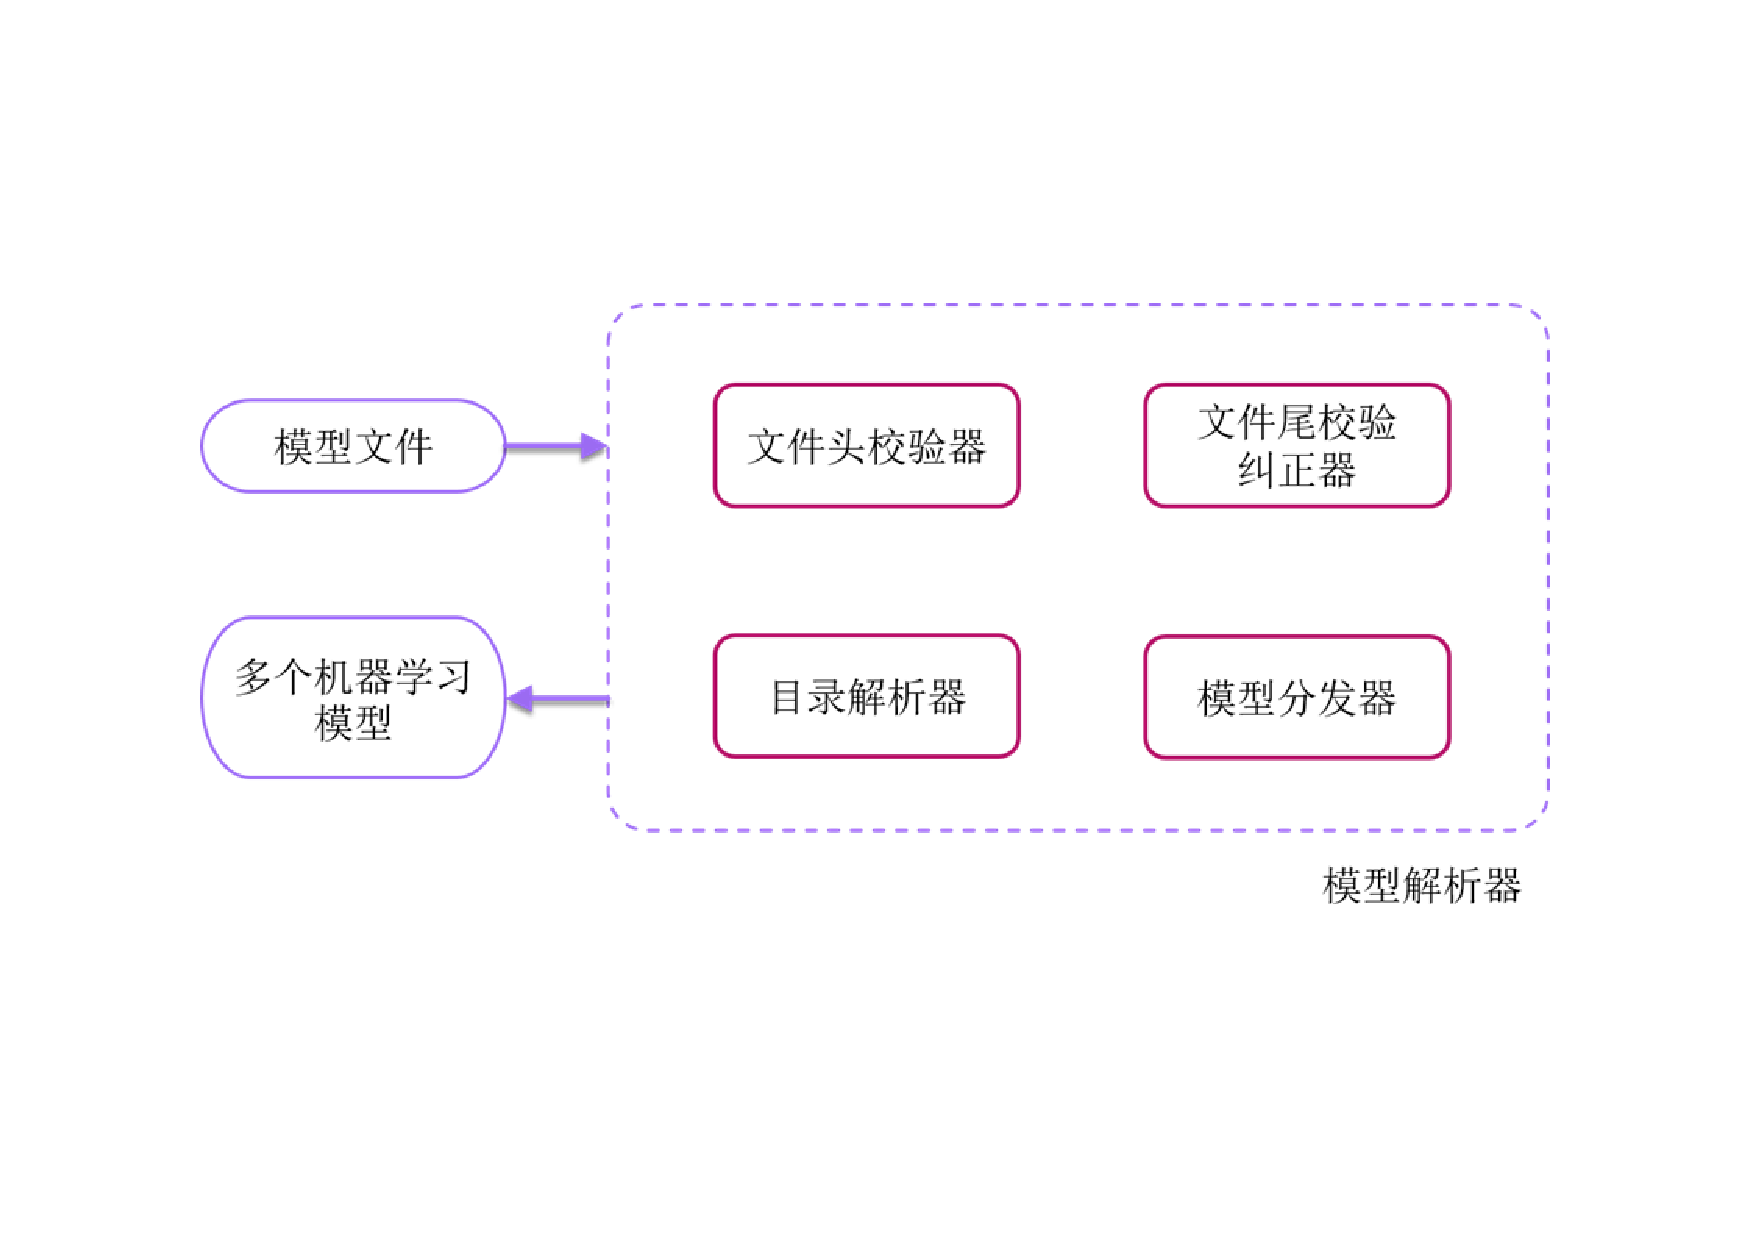
\includegraphics[width=0.8\textwidth]{model_praser.pdf}
  \caption{模型解析器}
  \label{fig:model_praser}
\end{figure}

各部分功能如下:

\begin{itemize}
  \item 文件头检验器用于读取模型文件,在文件头中找到文件标识码,检查是否合法,若合法则进入下一步,若不合法则向用户报告错误信息,解析过程停止;
  \item 文件尾校验器用于在文件尾中找到校验码,按照生成方法中相同的校验码算法,计算文件尾之前所有内容的校验码,比较本校验码与文件尾存储的校验码是否一致,若一致进行下一步,若不一致则说明文件损坏,向用户报告错误信息,解析过程停止;
  \item 目录解析器用于读取文件目录区,依次读取每个序列化后的模型,传给模型分发器;
  \item 模型分发器用于接收一个序列化后的模型,按照反序列化算法得到通用机器学习模型(kernel),然后读取通用机器学习模型中的硬件参数信息(硬件类别及型号),然后在设备池中搜索;若找到匹配硬件,则将机器学习模型发送给对应设备,由模型执行器控制后续在硬件设备上执行的过程;若找不到匹配硬件,则向用户报告错误信息,解析过程停止。(设备池可以是本机包含的计算部件,如CPU、GPU、专用处理器等,也可以是网络上可访问并可使用的计算机和计算部件)
\end{itemize}

\subsection {接口设计}

该模块对外接口的主要接口及其功能如表~\ref{tab:savemodel-interface-tab}所示。

\begin{table}[htb]
  \centering\small
  \caption{指令保存和加载模块对外接口}
  \label{tab:savemodel-interface-tab}
  \resizebox{0.6\textwidth}{36mm}{
  \begin{tabular}{ll}
    \toprule
    函数名       & saveModelToFile   \\
    \midrule
    输入 & 编译后生成的kernel \\
    输出 & 保存kernel的离线文件 \\
    功能 & 将编译后生成的指令保存到文件中\\
    说明 & 按文件设计格式填写内容 \\
    \bottomrule
    \toprule
    函数名       & loadModelFromFile    \\
    \midrule
    输入 & 离线模型的文件名 \\
    输出 & 反解析生成的kernel \\
    功能 & 从指令文件中解析出对应的kernel \\
    说明 & 解析前应做文件的完整性校验 \\
    \bottomrule
  \end{tabular}}
\end{table}

\section {权值替换模块}

\subsection {功能概述}

权值替换模块的主要目的是保持离线文件中Kernel的其它部分信息不变,只替换其权值信息的内容。该功能在网络结构信息相同,权值信息不同的时候用来替换离线模型文件中的权值数据,避免二次编译。

\subsection {设计思路}

权值信息不同肯定是Tensor绑定的数据发生了变化,由于我们并没有真正缓存权值信息对应的Json文件,而是只保存了一张权值信息表,所以我们没办法查找出具体是哪一个Tensor绑定的数据发生了变化,所以进行权值替换的时候需要将所有kernel中绑定的权值数据都进行替换。

kernel结构中包含了每个tensor的唯一标识符(name\_属性值)和绑定的静态数据信息。可以根据Tensor的名称,到kernel中找到其对应的数据,进行替换。

Tensor的name\_的属性值可以由用户通过接口显示设定,如果用户没有设定,则使用默认值,用操作名称和Tensor类型组成。如conv操作的FilterTensor默认名称是conv\_filter,conv操作的BiasTensor默认名称是conv\_bias。

\subsection {接口设计}
该模块对外接口的主要接口及其功能如表~\ref{tab:weight-replace}所示。

\begin{table}[htb]
  \centering\small
  \caption{权值替换模块对外接口}
  \label{tab:weight-replace}
  \begin{tabular}{ll}
    \toprule
    函数名       & replaceStaticData   \\
    \midrule
    输入 & 新绑定的权值数据 \\
    输出 & 更新静态数据后的kernel \\
    功能 & 更新kernel中的静态数据  \\
    说明 & 用户想要更新静态数据,必须明确指定待更新的tensor的name \\
    \bottomrule
  \end{tabular}
\end{table}

\section {权值量化模块}

\subsection {功能概述}
权值量化模块的主要功能是对浮点类型的权值数据做量化,用存储空间更小的int8或者int4类型来量化浮点数据,保证对神经网络进度影响不大的情况下,减少神经网络模型的体积,提高对缓存空间的利用率和神经网络的推理速度。

\subsection {设计思路}
现代计算机中,浮点数一般采用IEEE指定的国际标准表示,这种标准用三部分表示一个浮点数,如图~\ref{fig:float-data}所示。

\begin{figure}[htb]
  \centering
  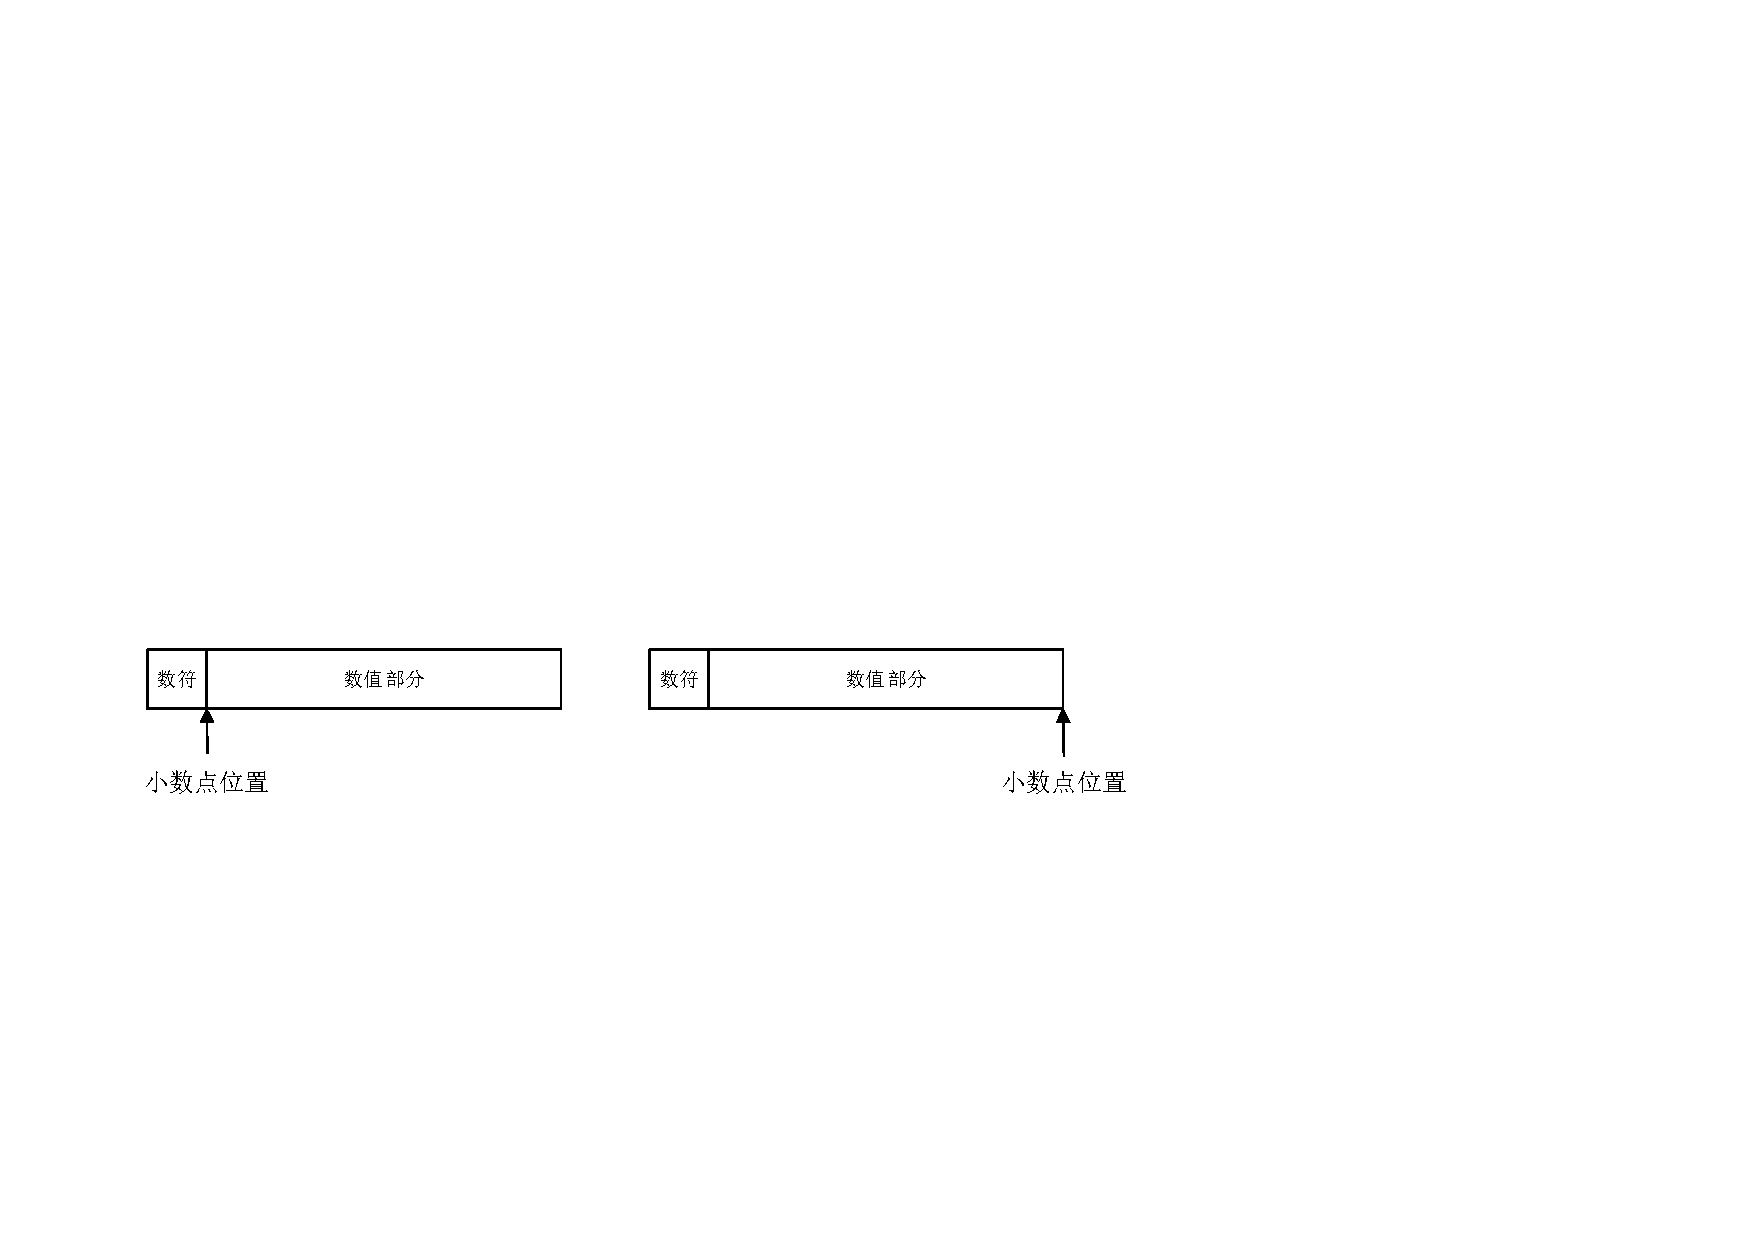
\includegraphics[width=0.8\textwidth]{float_data.pdf}
  \caption{浮点数存储示意图}
  \label{fig:float-data}
\end{figure}

数符表示浮点数的正负,用1位表示,0代表正数,1代表负数。阶码表示对浮点数进行加权,权重是2的阶码次幂,阶码的实际编码用移码表示,阶码的真实值都被加上一个常数(偏移量,float32的偏移量是127,float16的偏移量是15)后编码。尾数部分通常是规格化表示,即非0的有效位最高位总是1,但是在IEEE标准中通常会将规范化二进制浮点数整数位的1省略,称隐藏位,这样在有限的位数下,尾数可以多出一个精度位。表~\ref{tab:float32-tab}列出了十进制数178.125的实数表示。

\begin{table}[htb]
  \centering\small
  \caption{实数178.125的几种不同表示}
  \label{tab:float32-tab}
  \begin{tabular}{ll}
    \toprule
    实数表示       & 数值   \\
    \midrule
    原始十进制数   & 178.125 \\
    对应的二进制数 & 10110010.001 \\
    二进制浮点表示 & $1.0110010001^{111} $\\
    float32表示  & 符号位:0 \\ 
                 & 阶码:00000111+01111111=10000110 \\ 
                 & 尾数:01100100010000000000000(整数位1隐藏)\\
    \bottomrule
  \end{tabular}
\end{table}

小数点固定在某一位置的数称为定点数,有两种方式,如图~\ref{fig:int-data}所示。

\begin{figure}[htb]
  \centering
  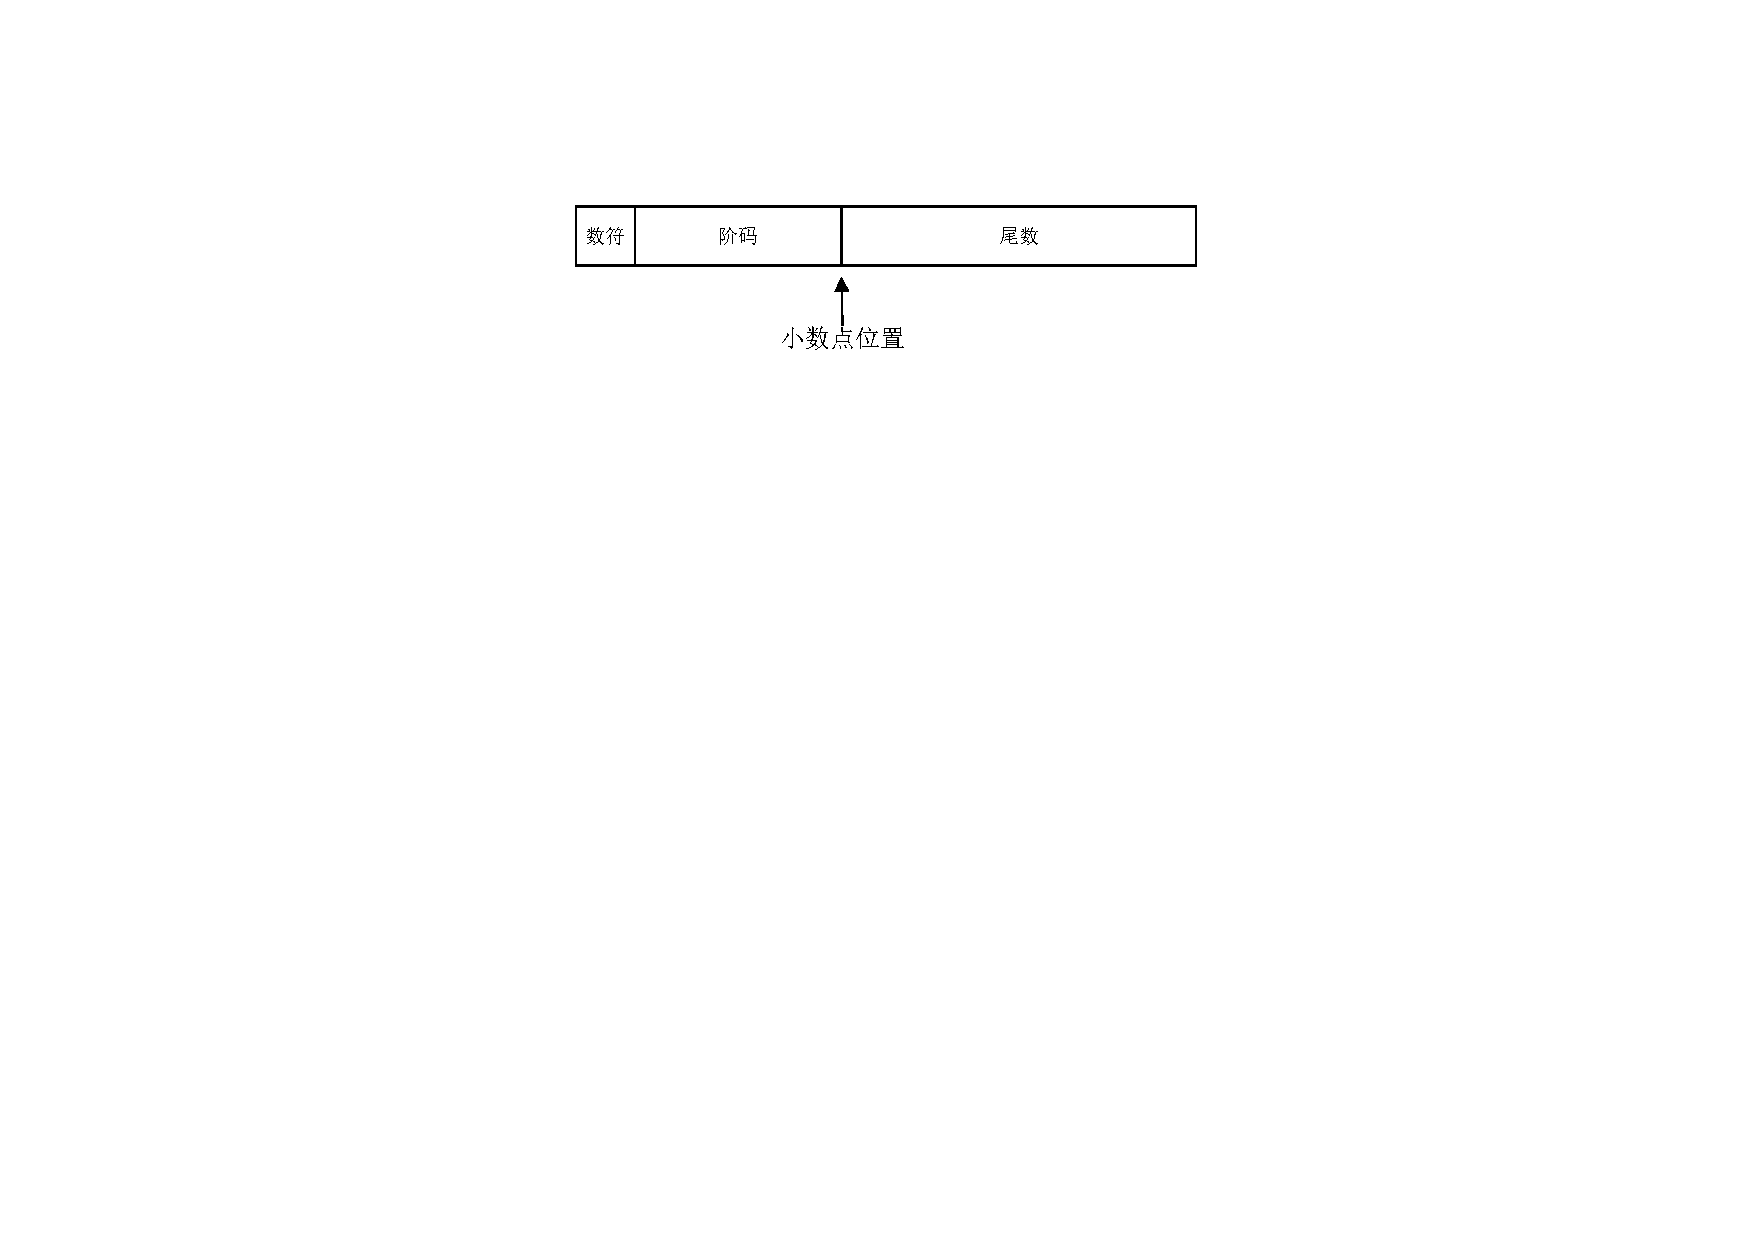
\includegraphics[width=0.6\textwidth]{int_data.pdf}
  \caption{定点数存储示意图}
  \label{fig:int-data}
\end{figure}

当小数点位于数符和第一数值位之间时为纯小数;当小数点位于数值位之后时为纯整数,数值部分的位数n决定了定点数的表示范围。如果忽略计算机内部正零和负零的表示约定,认为正零和负零是有区别的,那么纯小数的表示范围是[-(1-$2^{-n}$),1-$2^{n}$],纯整数的表示范围是[{-($2^{n}$-1}),{$2^{n}$ -1}]。

在定点数中,由于小数点的位置固定不变的,所以不能直接表示不是纯小数或者纯整数的数。但是如果我们让定点数共享一个指数,然后乘以一个比例因子,就可以表示浮点数了。

\begin{equation}
  r_x \approx q_x \times 2^{position} \times scale
\end{equation}

上述公式中,$r_x$表示真实的浮点数,$q_x$表示量化后的数值,$position$表示共享的指数,$scale$表示缩放系数。对一组浮点数进行量化的过程就是计算量化参数的过程。

\subsection {量化参数求解}

我们不妨假设对 $r_x \in \real^d$ 的实数采用n比特量化(n位纯整数),即采用n比特存储。$position$表示定点数的小数点位置,理论上在保证覆盖 $\real^d$中最大绝对值的基础上,小数点越靠左越好(小数点越靠左,精度越高),即 $position$越小越好。所以 $position$ 应该满足以下两个约束\\

\begin{equation}
  {(2^{n-1} - 1)} \times 2^{position} \ge \max r_x 
\end{equation} 

\begin{equation}
  {(2^{n-1} - 1)} \times 2^{position - 1} < \max r_x 
\end{equation} 

n比特能表示的最大的数是$2^{n-1} - 1$,量化后能表示的最大值覆盖所有需要量化的实数,又不能过大。所以\\

\begin{equation}
 log_2 {\frac {\max r_x}{2^{n-1} -1}} \le position < log_2 {\frac {\max r_x}{2^{n-1} -1}} +1
\end{equation} 
所以可以得出\\
\begin{equation}
 position = \left \lceil log_2 {\frac {\max r_x}{2^{n-1} -1}} \right \rceil  
\end{equation} 
并且可以继续推理出\\

\begin{equation}
 \frac{1}{2} < \frac {\max r_x}{{(2^{n-1} -1)} \times 2^{position}} \le 1  
\end{equation} 

其中${(2^{n-1} -1)} \times 2^{position}$表示量化能取到的最大值,然而值和实际的最大值之间有一定的差距,为了更精确的表示量化之前的数据,我们可以增加一个缩放系数$scale$来调节。所以 \\

\begin{equation}
 scale = \frac {\max r_x}{{(2^{n-1} -1)} \times 2^{position}} \Rightarrow scale \in (\frac{1}{2} \text, 1]
\end{equation} 

\subsection{接口设计}
该模块对外接口的主要接口及其功能如表~\ref{tab:weight-quant-tab}所示。

\begin{table}[htb]
  \centering\small
  \caption{权值量化模块对外接口}
  \label{tab:weight-quant-tab}
  \begin{tabular}{ll}
    \toprule
    函数名       & getPositionAndScale                \\
    \midrule
    输入 & 待量化的一组浮点数,指令量化结果类型           \\
    输出 & 量化参数position,scale的值                   \\
    功能 & 求出量化到指定类型所需要的量化参数              \\
    说明 & 量化结果类型是一个枚举变量,支持量化到不同的整型 \\
    \bottomrule
    \toprule
    函数名       & quantifyBindData              \\
    \midrule
    输入 & 用户的权值的原始数据,量化参数           \\
    输出 & 量化后的数据                            \\
    功能 & 将用户原始绑定的数据根据量化参数求进行量化 \\
    说明 & 指令文件中同时保存量化后的数据和量化参数   \\
    \bottomrule
  \end{tabular}
\end{table}

\section {本章小结}

本章主要介绍了整个框架的概要设计,根据需求分析划分出各个功能模块,然后描述了模块的主要功能,设计思路和对外接口,同时描述了系统的整体运行流程,各个模块之间的联系和依赖。通过整体的流程图和各个模块的对外接口,描述整体的实现过程和方式,为后序详细的设计奠定基础。
% !TeX root = ../main.tex

\chapter{详细设计与实现}

本章将在第4章的基础上对划分出来的各个模块进行更为详细的设计与实现。一方面通过类图的形式,展现在本模块中各个类之间的关系,通过类的属性和接口设计,相互配合完成本模块的功能;另一方面,对于比较复杂重要的方法实现,采用流程图的形式,详细介绍其内部的实现逻辑和流程。

\section{图信息保存模块设计与实现}

图信息保存模块是整个编译优化中避免重复编译的基础,只有在能保存下用户图信息的基础上,才能继续实现图信息识别和指令替换等功能。图信息保存模块要实现将操作的结构和数据信息保存到对应的Json对象,最后将Json像的内容转输出成可读的Json文件,该模块类图设计如图~\ref{fig:info-save-model}所示。

\begin{figure}[htb]
  \centering
  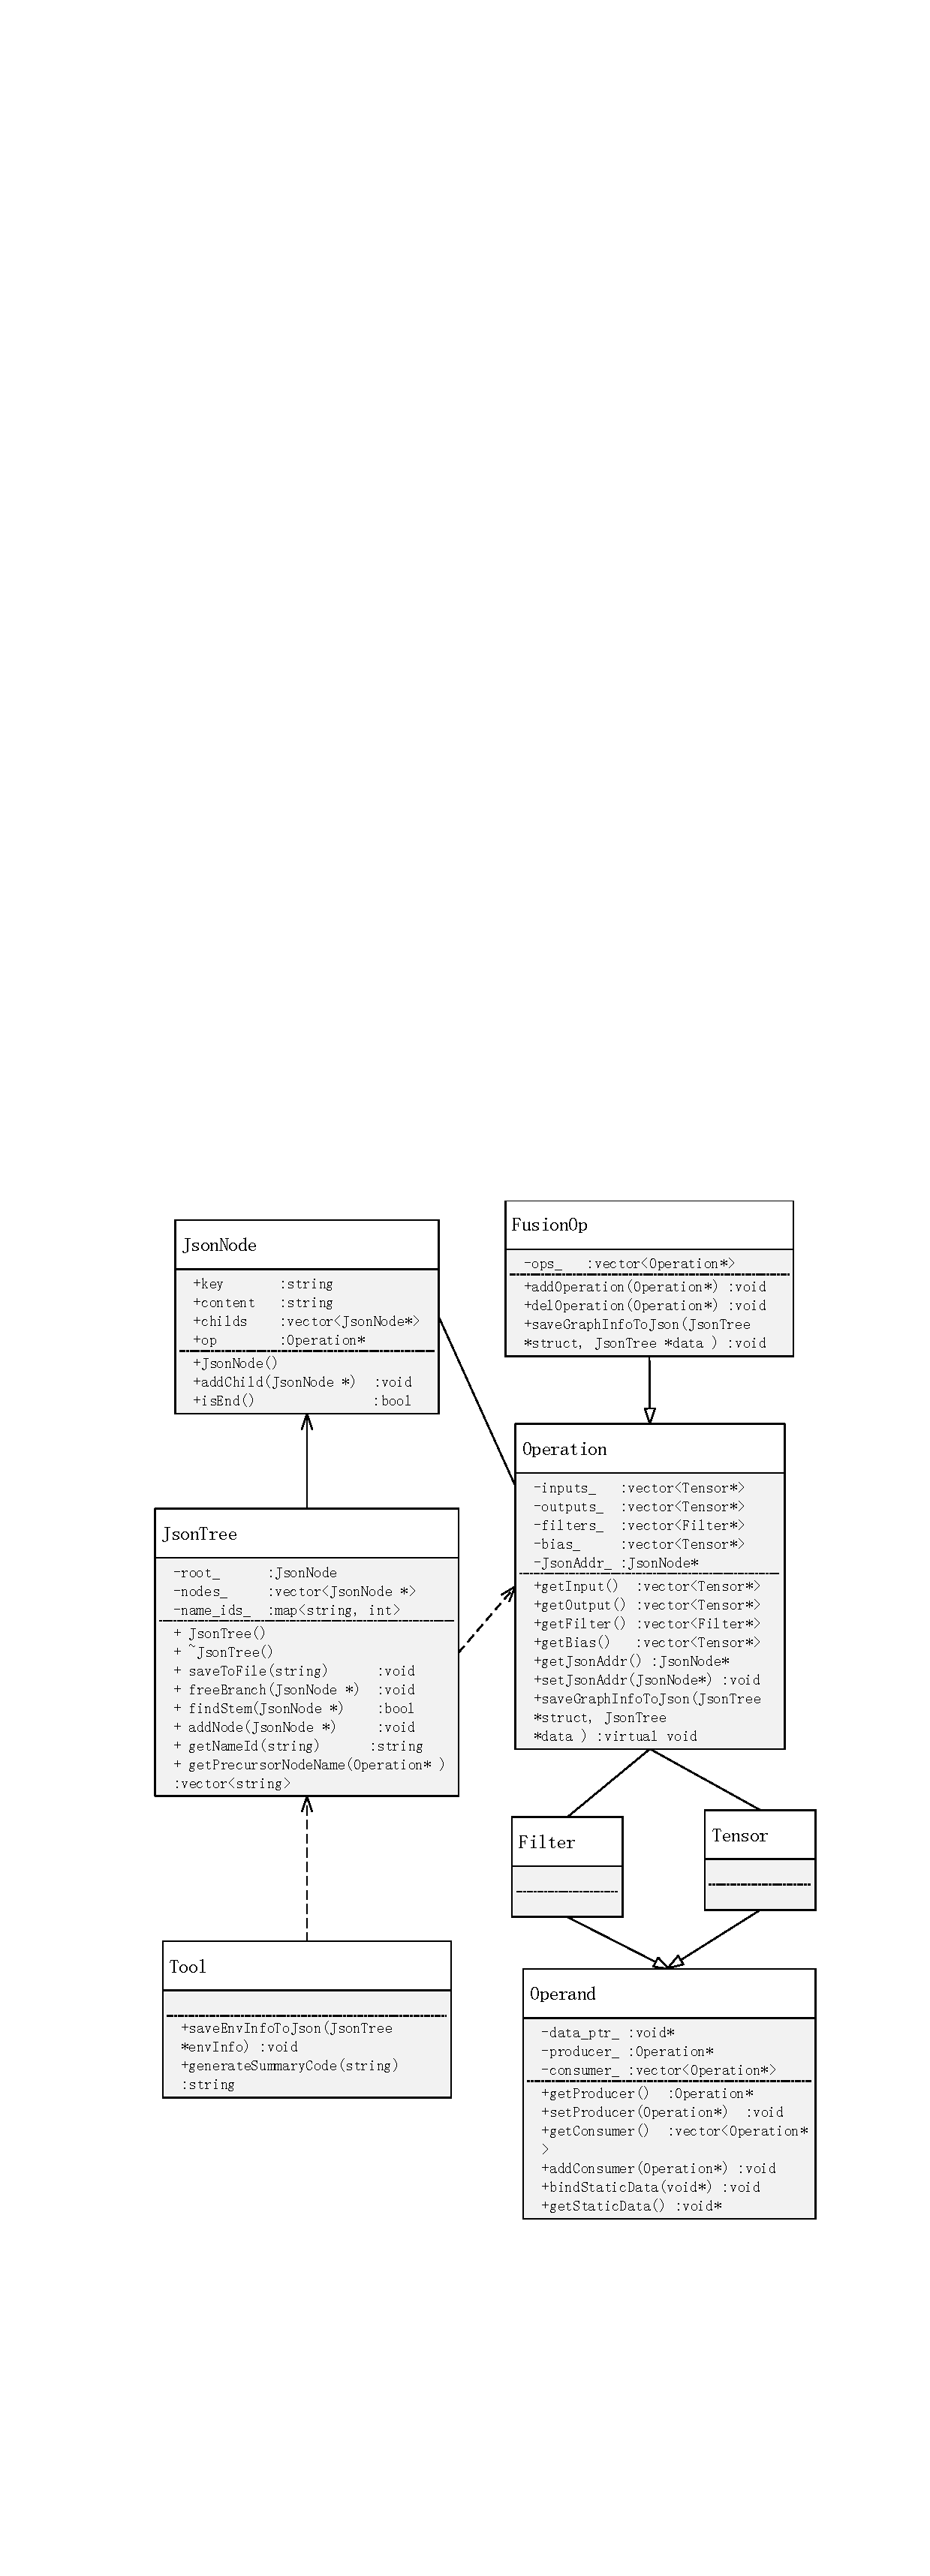
\includegraphics[width=0.6\textwidth]{info_save_model.pdf}
  \caption{图信息保存模块类图}
  \label{fig:info-save-model}
\end{figure}

各个类主要函数的功能在表~\ref{tab:function-list}中做了简要说明。
\begin{table}[htb]
  \centering\tiny
  \caption{函数功能表}
  \label{tab:function-list}
  \begin{tabular}{llll}
    \toprule
    类名        & 函数名     & 功能      & 说明                \\
    \midrule
    JsonNode   & addChild  & 添加子节点     & 仅仅当content为空时才有效 \\
               & isEnd     & 判断是否是终点 & 保存到文件中是用来判读是否是结尾\\
    \midrule
    JsonTree   & saveToFile  & 将JsonTree的内容保存到文件中  &  \\
               & freeBranch  & 释放指定分支 & 析构时使用\\
               & saveStemToFile & 保存指定分支到文件中 & \\
               & addNode & 添加子节点 & \\
               & getNameId & 查找同类型的节点的数量& 输入操作的名称,字典name\_id\_对应该名称对应的个数 \\
               & getPrecursorNodeName & 查找指定操作所有前驱节点的name & 通过操作和Tensor来判断前驱和后继的关系\\ 
    \midrule
    FusionOp   & addOperation  & 向计算图中添加子操作    &  \\
               & delOperation  & 删除计算图中指定的操作 &  \\ 
               & saveGraphInfoToJson & 保存计算图的结构和数据信息 & 通过调用其中的子操作实现 \\
    \midrule
    Operation  & getInput   & 获取输入Tensor    &  \\
               & getOutput  & 获取输出Tensor &  \\ 
               & getFilter  & 获取filter & \\
               & getBias    & 获取bias  & \\
               & getJsonAddr& 获取操作对应JsonNode的指针 & \\
               & saveGraphInfoToJson & 保存结构信息到对应的JsonTree中 & 虚函数,子类根据自身实际情况实现 \\
               & saveDataInfoToJson & 保存静态数据信息到JsonTree中 & 在基类中实现 \\
    \midrule
    Tool       & saveEnvInfoToJson   & 保存环境信息到JsonTree中  \\
               & generateSummaryCode & 根据输入内容生成信息摘要编码  &使用MD5码算法实现,返回长16个字符的编码\\
    \midrule
    Operand    & getProducer  & 找操作数的生产者  &每个操作数只有一个生产者,即它只能是/一个操作的输出 \\
               & getConsumer  & 找操纵数的消费者  &每个操作可能有多个消费者,即它可以是多个操作的输入 \\
               & bindStaticData  & 绑定静态数据信息  & 静态数据信息的绑定应该在编译之前完成\\
               & getStaticData   & 获取静态数据地址  & \\ 
    \bottomrule 
  \end{tabular}
\end{table}

在~\ref{fig:info-save-model}的类图中可以看出,图信息实际上都是保存在JsonTree的实例化对像中。因为环境信息不依赖与任何操作而只与当前的运行环境相关,所以直接方法工具类Tool中实现,结构信息和权值信息都和操作相关,所以放到操作中实现。工具类Tool中还实现了另一个重要的方法generateSummaryCode,用于生成字符串对应的信息摘要编码。操作中保存图信息的入口是基类Operation中的虚函数saveGraphInfoToJson,子类操作实现该接口将自己的信息加入到JsonTree中。包含有多个操作的图用FusionOp表示,FusionOp的图信息保存通过遍历调用包含在其中的子操作对应的接口实现。

信息存在JsonTree中,而JsonTree实际上是由一个个的JsonNode组成,JsonNode可以有多种方式存放信息。如果是string-string类型的键值对,则可以直接用key和content保存内容;如果键值对中值的类型是一个或多个Json对象,则可以保存到childNodes中。这样就可以通过增加子节点的方式,逐级拓展下去。


\subsection {保存结构信息}
接下来详细介绍操作的saveGraphInfoToJson函数如何利用各种接口实现将计算图的结构信息存储到JsonTree中的,saveGraphInfoToJson实现步骤如流程图~\ref{fig:save-graph-info}所示。

\begin{figure}[htb]
  \centering
  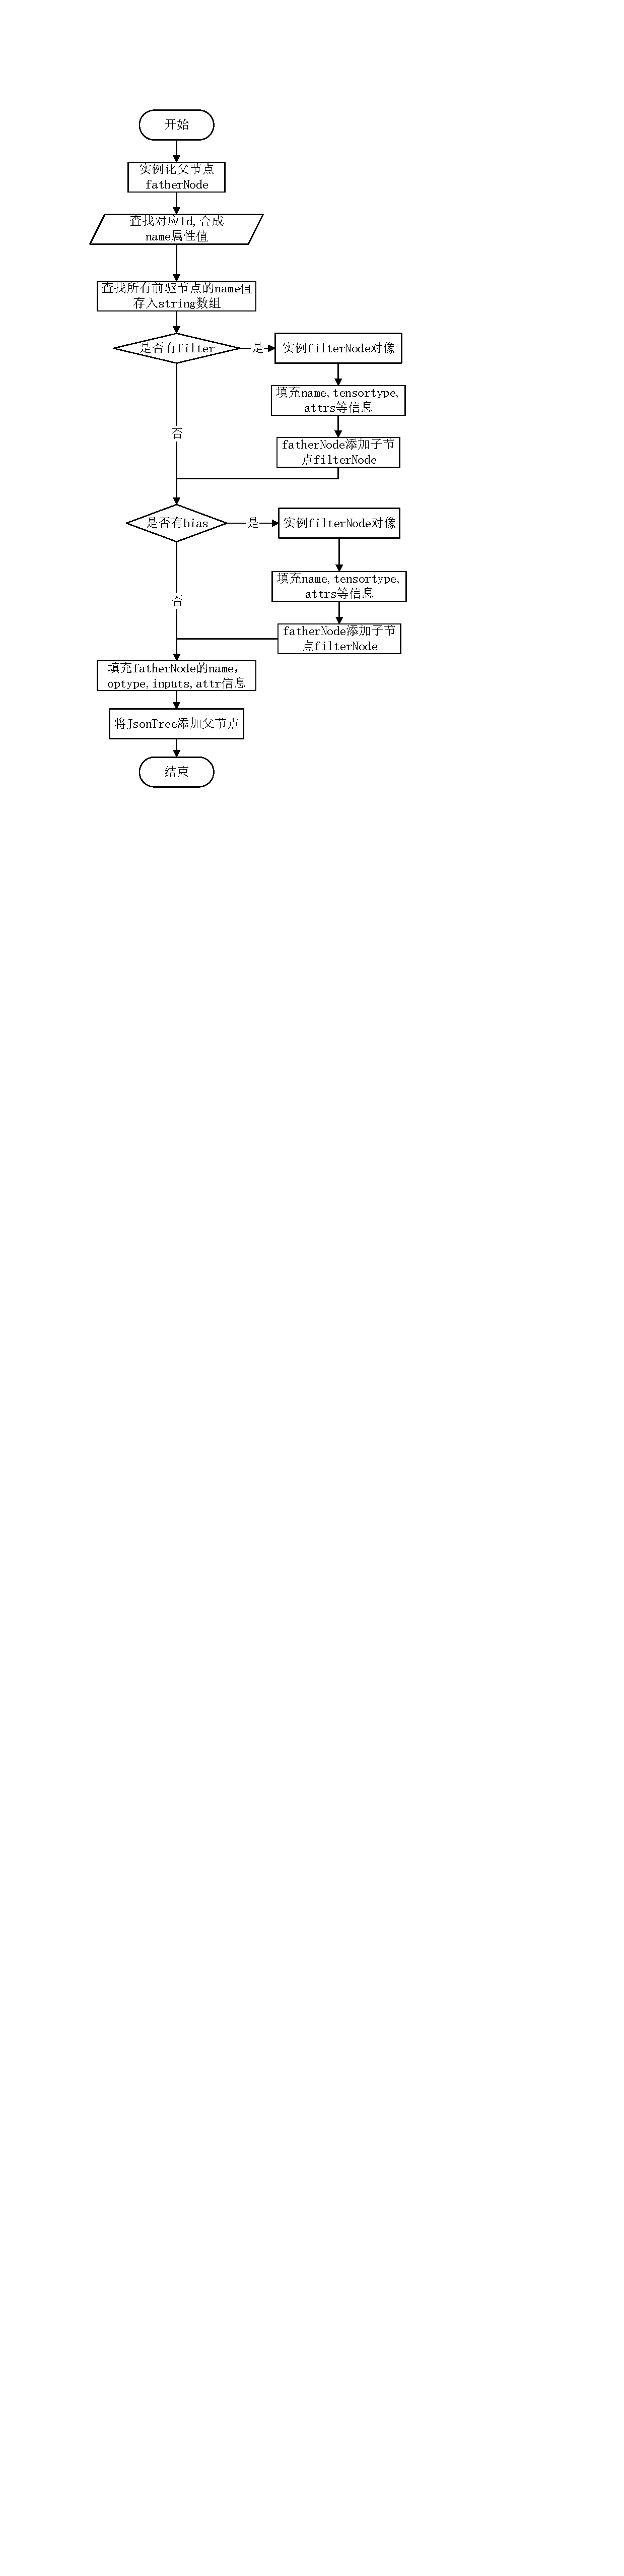
\includegraphics[width=0.4\textwidth]{save_graph_info.pdf}
  \caption{saveGraphInfoToJson流程图}
  \label{fig:save-graph-info}
\end{figure}

在图~\ref{fig:save-graph-info}中,每个操作都要实例化和直接对应一个JsonNode,实例化之后,Operation中的jsonAddr\_指向这个实例化的对象,同时JsonNode中的op指针也指向当前操作。唯一标识符name由类型名和Id号两部分组成,当JsonTree中出现多个conv类型节点时会以conv1,conv2…的形式命名,所以要查找当前Id来合成name。接下来较为麻烦的一步是需要查找出当前节点的输入来自于哪些节点,需要将这些节点的name信息写入到inputs中。然后根据操作输入是否存在filter和bias来决定是否需要添加filter和bias的信息,并将filter和bias的name值也写入到当前节点的inputs中。最后补充name,optype,attrs字段的信息,并将操作节点添加到JsonTree。

查找前驱节点是通过JsonTree的getPrecursorNodeName函数来实现,其逻辑如图~\ref{fig:get-precursor-node}所示。

\begin{figure}[htb]
  \centering
  \subfigure[getPrecursorNodeName流程图]{
  \label{fig:get-precursor-node}
  
\includegraphics[width=0.4\textwidth]{get_precursor_node.pdf}
  }
  \subfigure[保存权值流程图]{
  \label{fig:save-weight-info}
  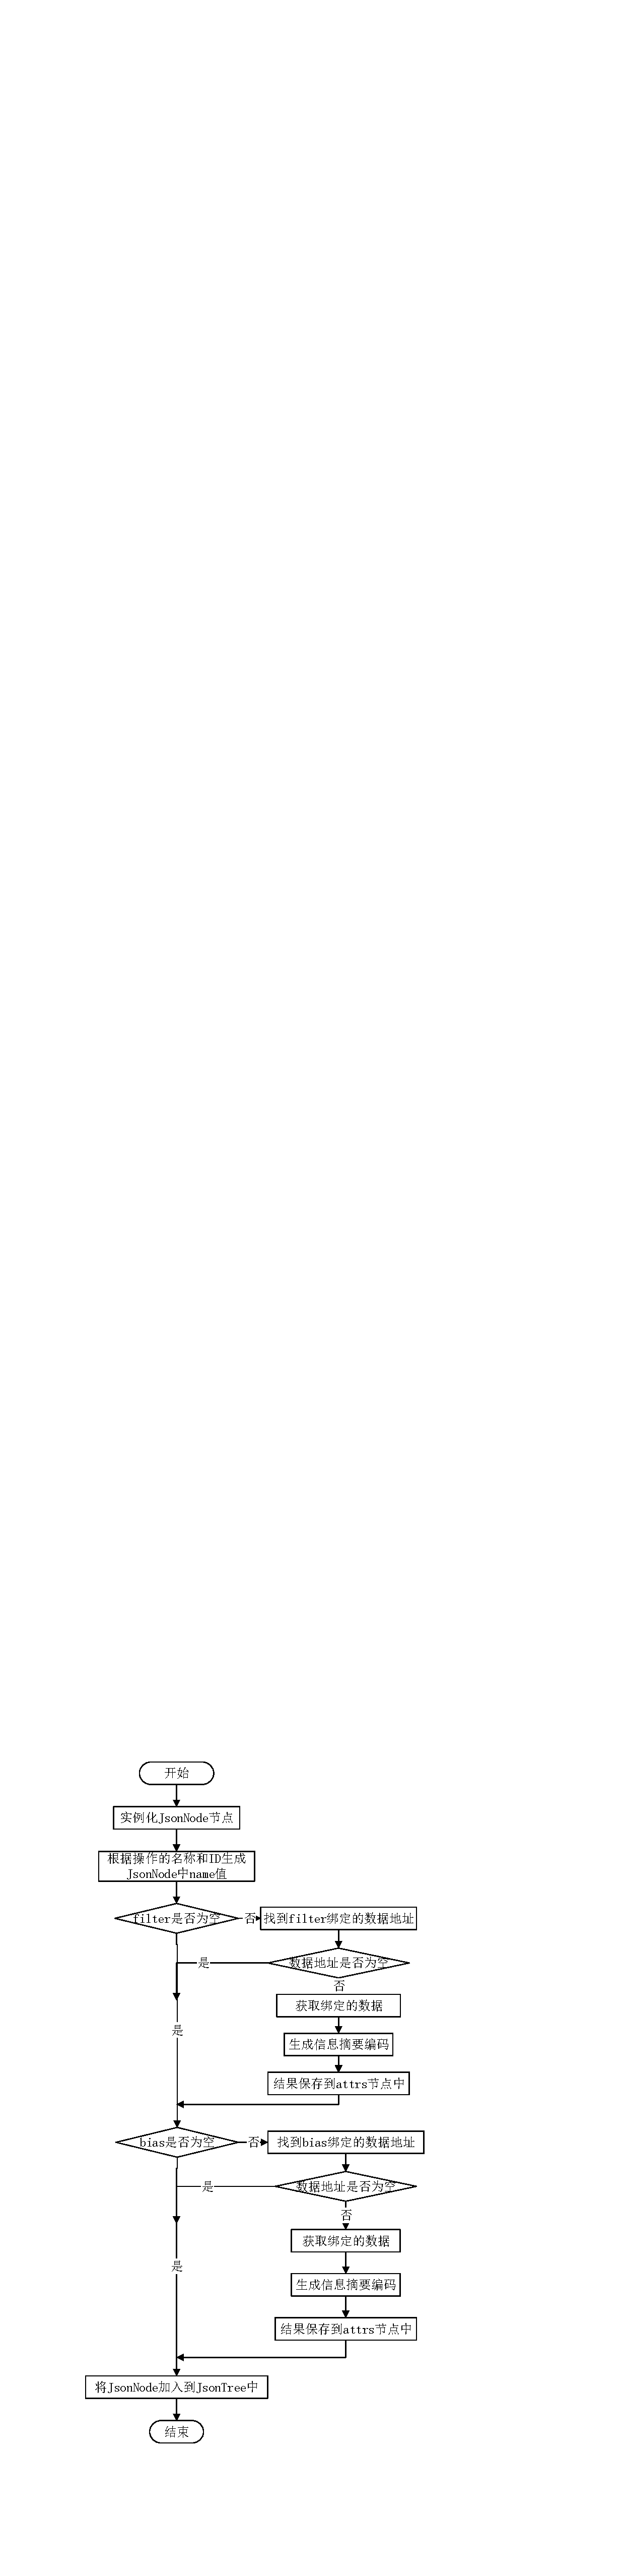
\includegraphics[width=0.5\textwidth]{save_weight_info.pdf}
  }
  \caption{保存结构信息的关键流程图}
  \label{fig:strcut-save-key}
\end{figure}

其实现的关键就是在JsonNode和Operation中保存了指向对方的指针。这样在生成JsonNode的时候可以利用Operation和tensor的关系来判断JsonNode的前驱和后继。如果输入Tensor没有生产者,肯定是神经网络的外部输入,数据在运行时由用户动态填充。

\subsection {保存权值信息}

与保存结构信息相比,保存权值信息就显得相对容易了。因为所有操作的静态书籍不是绑定在filter上就是绑定在bias上,所以所有操作保存权值信息的逻辑都是一样的,如图~\ref{fig:save-weight-info}所示。

首先还是根据操作类型生成唯一的标识name,然后根据是否存在filter和bias以及是否绑定了静态数据分别处理。如果绑定了静态数据,则找到静态数据,生成对应的信息摘要编码,保存到staticdata节点中。

\subsection {保存JsonTree到文件}

将JsonTree保存到文件中,关键就是将JsonTree中包含的JsonNode的内容按照Json的语法规则写入到文件中,。Json语法规则的语法规则如下:
\begin{itemize}
  \item 数据在名称/值对中
  \item 数据由逗号分隔
  \item 花括号保存对象
  \item 方括号保存数组
\end{itemize}
应用到JsonNode,可以分为以下4种情况:
\begin{enumerate}
  \item 当key和content都不为空时,“key”:“content”;
  \item 当key不为空,content为空时,“key”:[childNode] ;
  \item 当key为空,content不为空时,“content”(用于保存前驱节点name的情况);
  \item 当key和content均为空时,{childNode}
\end{enumerate}
在JsonTree的saveToFile函数中,遍历nodes\_,对其中的每个JsonNode调用递归函数saveStemToFile, 递归出口是JsonNode中childNode的大小为0。函数体的主要内容就是判断JsonNode属于上面所述的哪一种情况,然后将内容保存到stringstream中。最后将stringstream写入文件即可。

\section{图信息识别模块设计与实现}
根据JsonTree生成的Josn文件也会占用大量的存储空间,为了节省缓存空间,不直接保存JsonTree生成的Json文件(在调试情况下可以保存下来,方便查看网络结构),而是根据Json文件的内容生成对应的信息摘要编码,保存信息摘要编码后删除对应的Json文件。查找的时候到对应的缓存表中查找是否用相同的信息摘要编码即可。设计到主要的类和方法如图~\ref{fig:graph-info-check}所示。

\begin{figure}[htb]
  \centering
  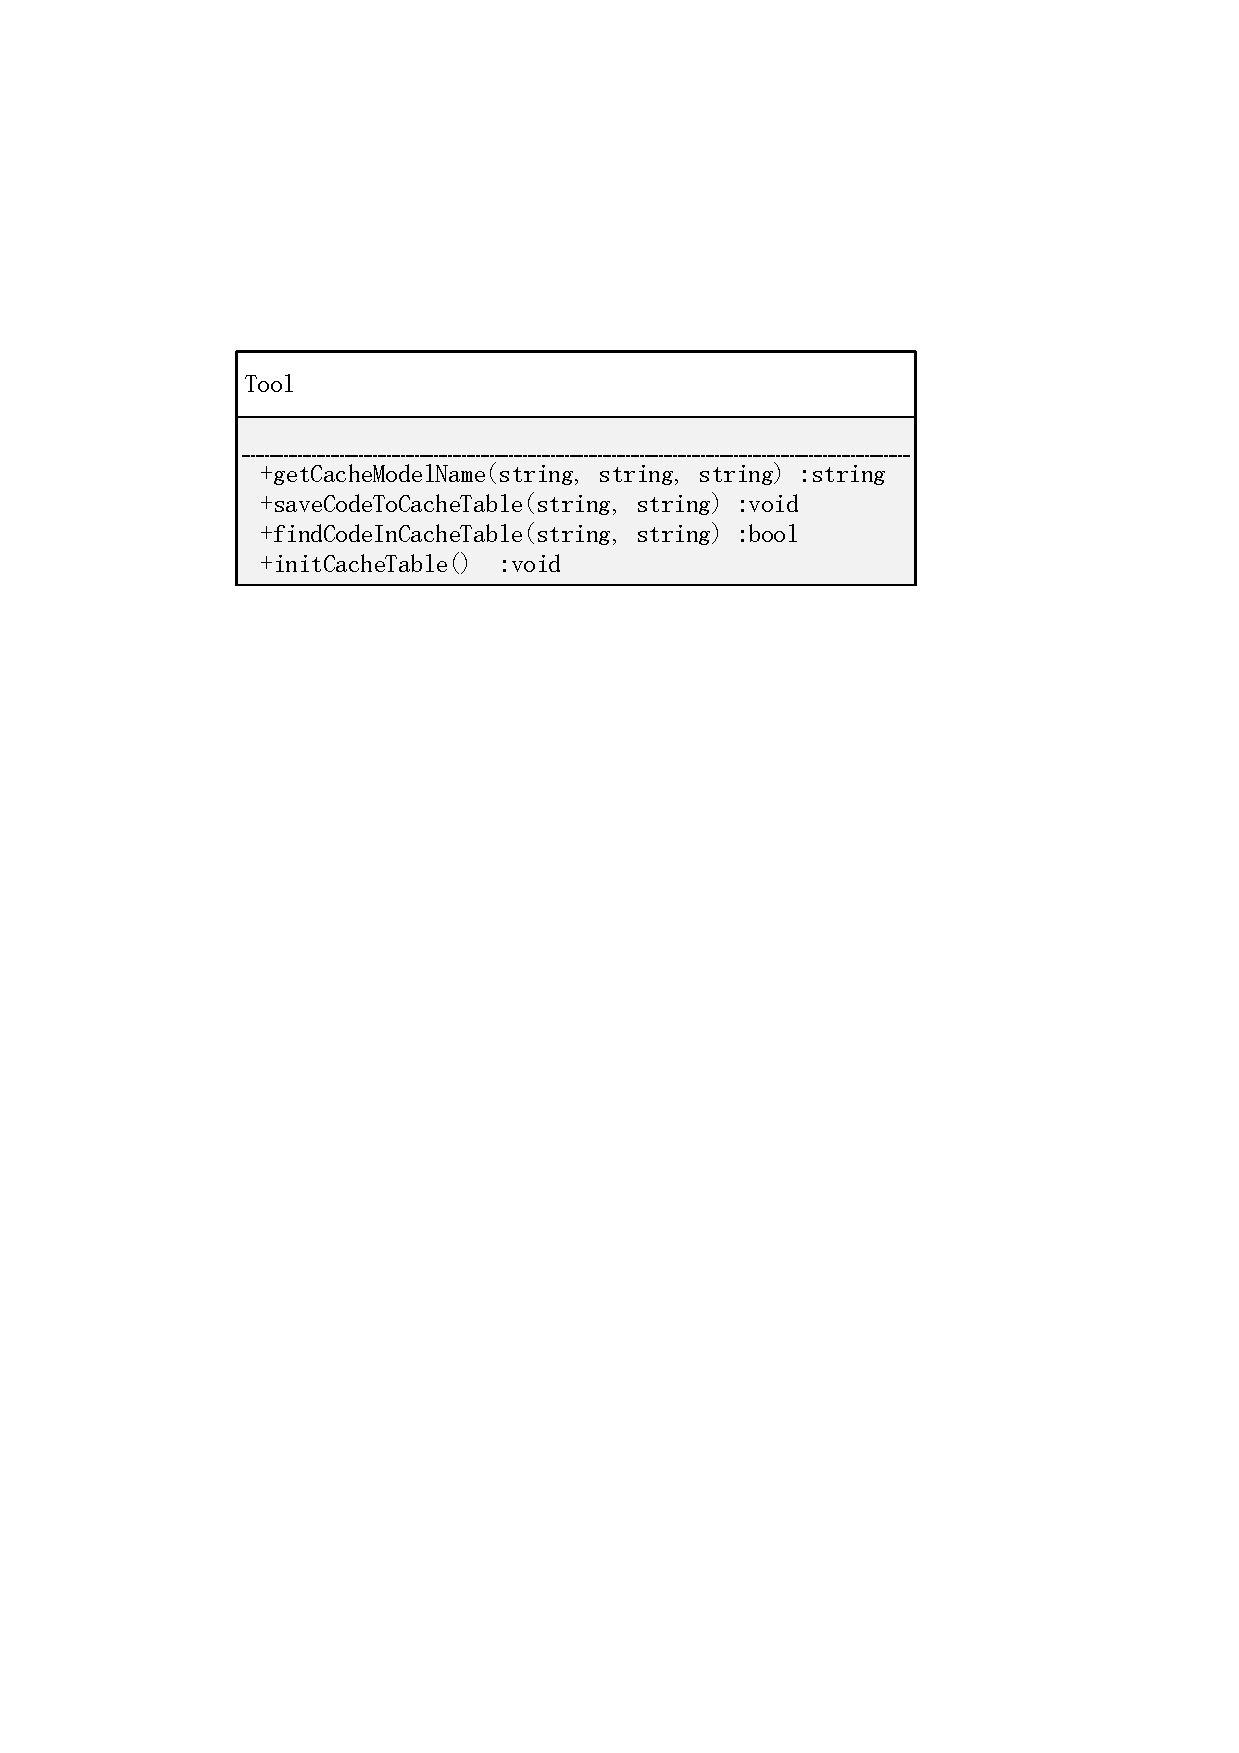
\includegraphics[width=0.5\textwidth]{graph_info_check.pdf}
  \caption{图信息识别模块类图}
  \label{fig:graph-info-check}
\end{figure}

函数功能简介见表~\ref{tab:function-desc-tab}。

\begin{table}[htb]
  \centering\small
  \caption{图信息识别函数功能表}
  \label{tab:function-desc-tab}
  \begin{tabular}{lll}
    \toprule
    函数名      & 功能   & 说明                       \\
    \midrule
    initCacheModel       & 初始化缓存表  & 初始化三张缓存表  \\
    saveCodeToCacheTable & 将摘要编码保存到指定的文件中 &     \\
    findCodeInCacheTable & 在指定的文件中查找指定的摘要编码  & \\
    getCacheModelName & 查找满足要求的指令缓存文件名  & 找到返回文件名,\\
                                                  &&没找到返回空字符串 \\
    \bottomrule
  \end{tabular}
\end{table}

初始化缓存表时初始化三张缓存表,分为是保存环境信息编码的version\_table,保存结构信息编码的struct\_table保存权值信息的data\_table。图识别功能由getCacheModelName函数实现,其流程如图~\ref{fig:get-cache-model}所示。

\begin{figure}[htb]
  \centering
  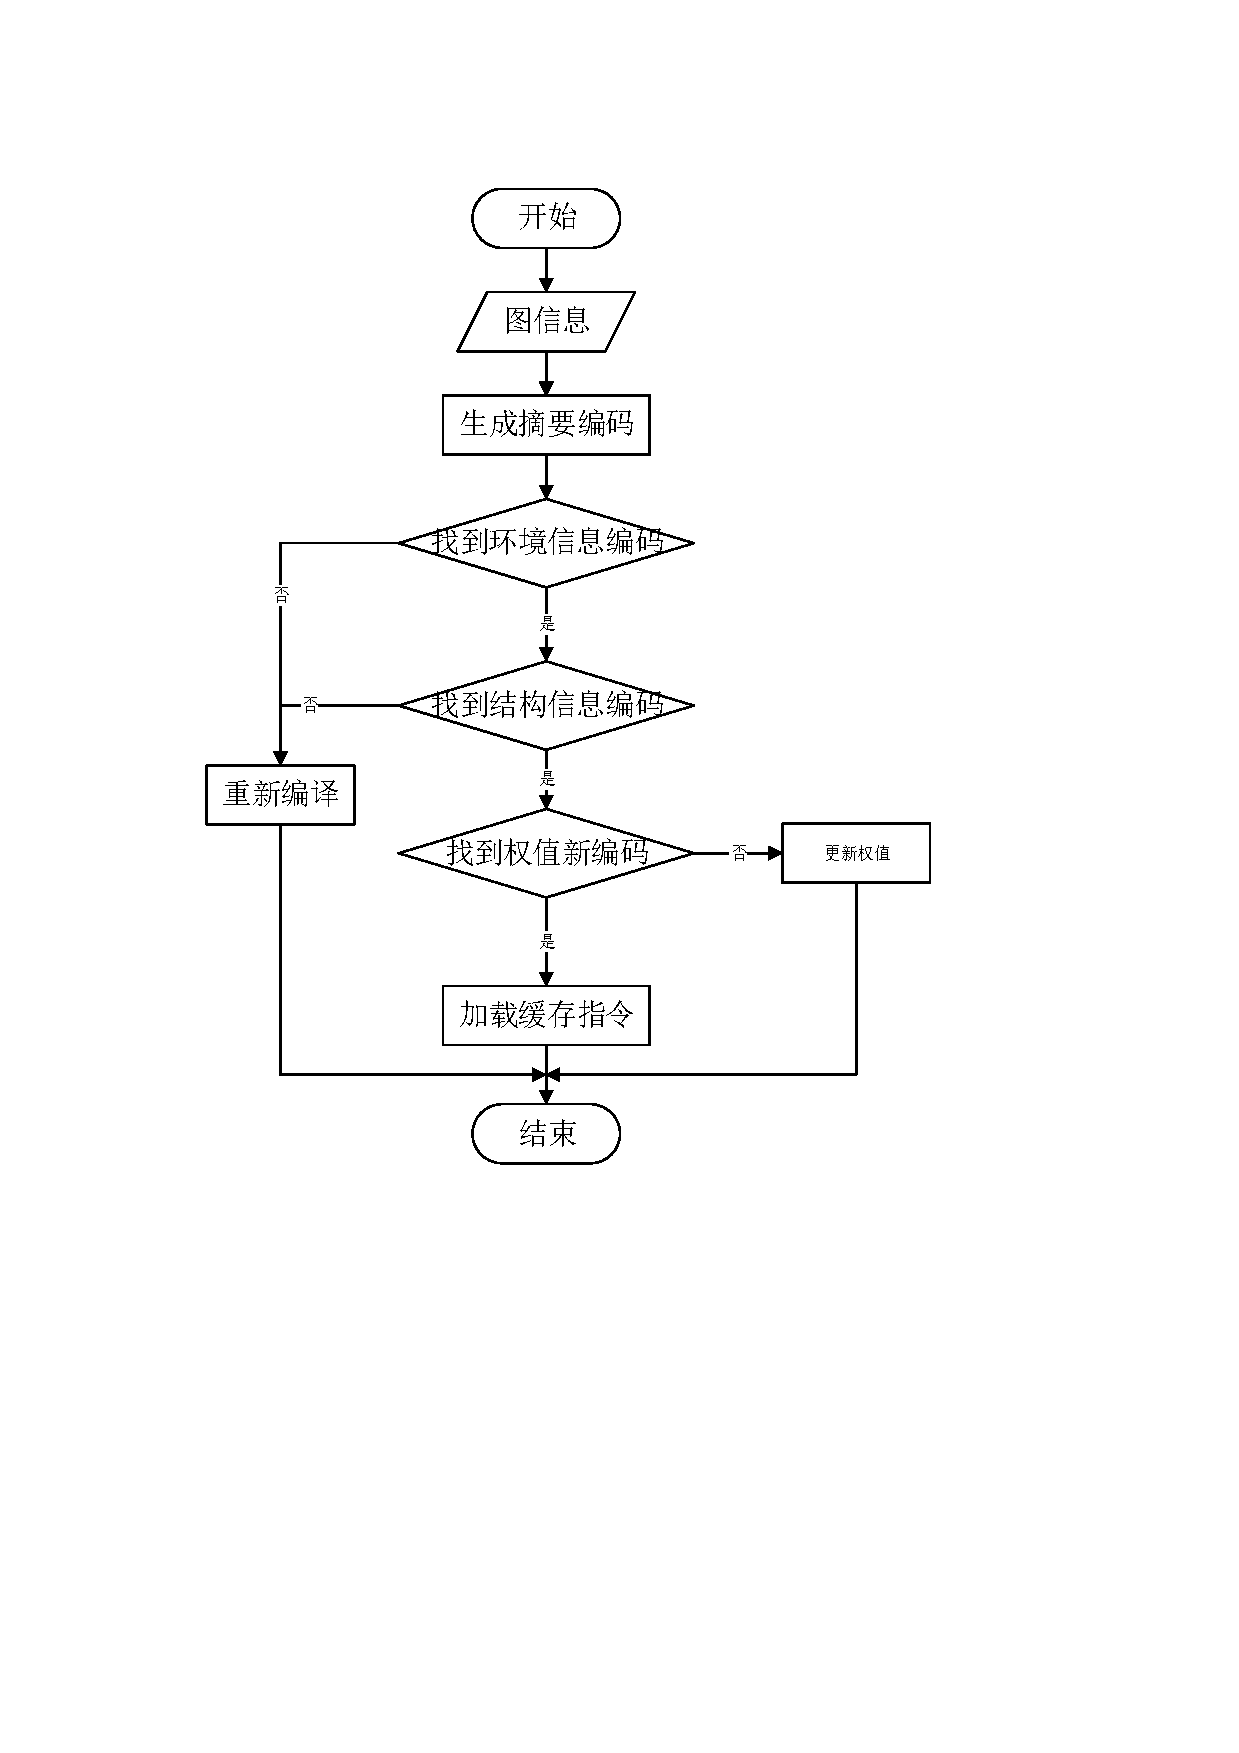
\includegraphics[width=0.5\textwidth]{get_cache_model.pdf}
  \caption{图信息识别模块类图}
  \label{fig:get-cache-model}
\end{figure}

比较的时候只先根据信息摘要算法对三部分信息生成对应的摘要编码,然后在version\_table中查找是否有当前的环境信息编码,没有代表编译环境发生了变化,需要重新编译;如果当前环境信息摘要编码存在于环境信息表,则继续在struct\_table中查找结构信息摘要编码,如果没找到,重新编译;如果找到则继续在data\_table中查找权值信息摘要编码,如果找到,则说明已经缓存了一份满足条件的指令,直接加载这份指令即可,如果只是权值信息编码没有找到,则拿一份结构相同的指令进行权值替换,也不需要重复编译。

\section{指令保存和加载模块设计与实现}
该模块设计的主要任务是将kernel离线保存到文件然后在需要的时候从文件中解析出之前保存的kernel。由于不同平台的kernel可以有很多不同的结构和设计方式,并且kernel的详细结构和功能对本模块的影响不大。所以本模块将淡化kernel的详细设计,而将重点放在如何实现指令的保存和加载上。类之间的关系如图~\ref{fig:load-cache-class}所示。

\begin{figure}[htb]
  \centering
  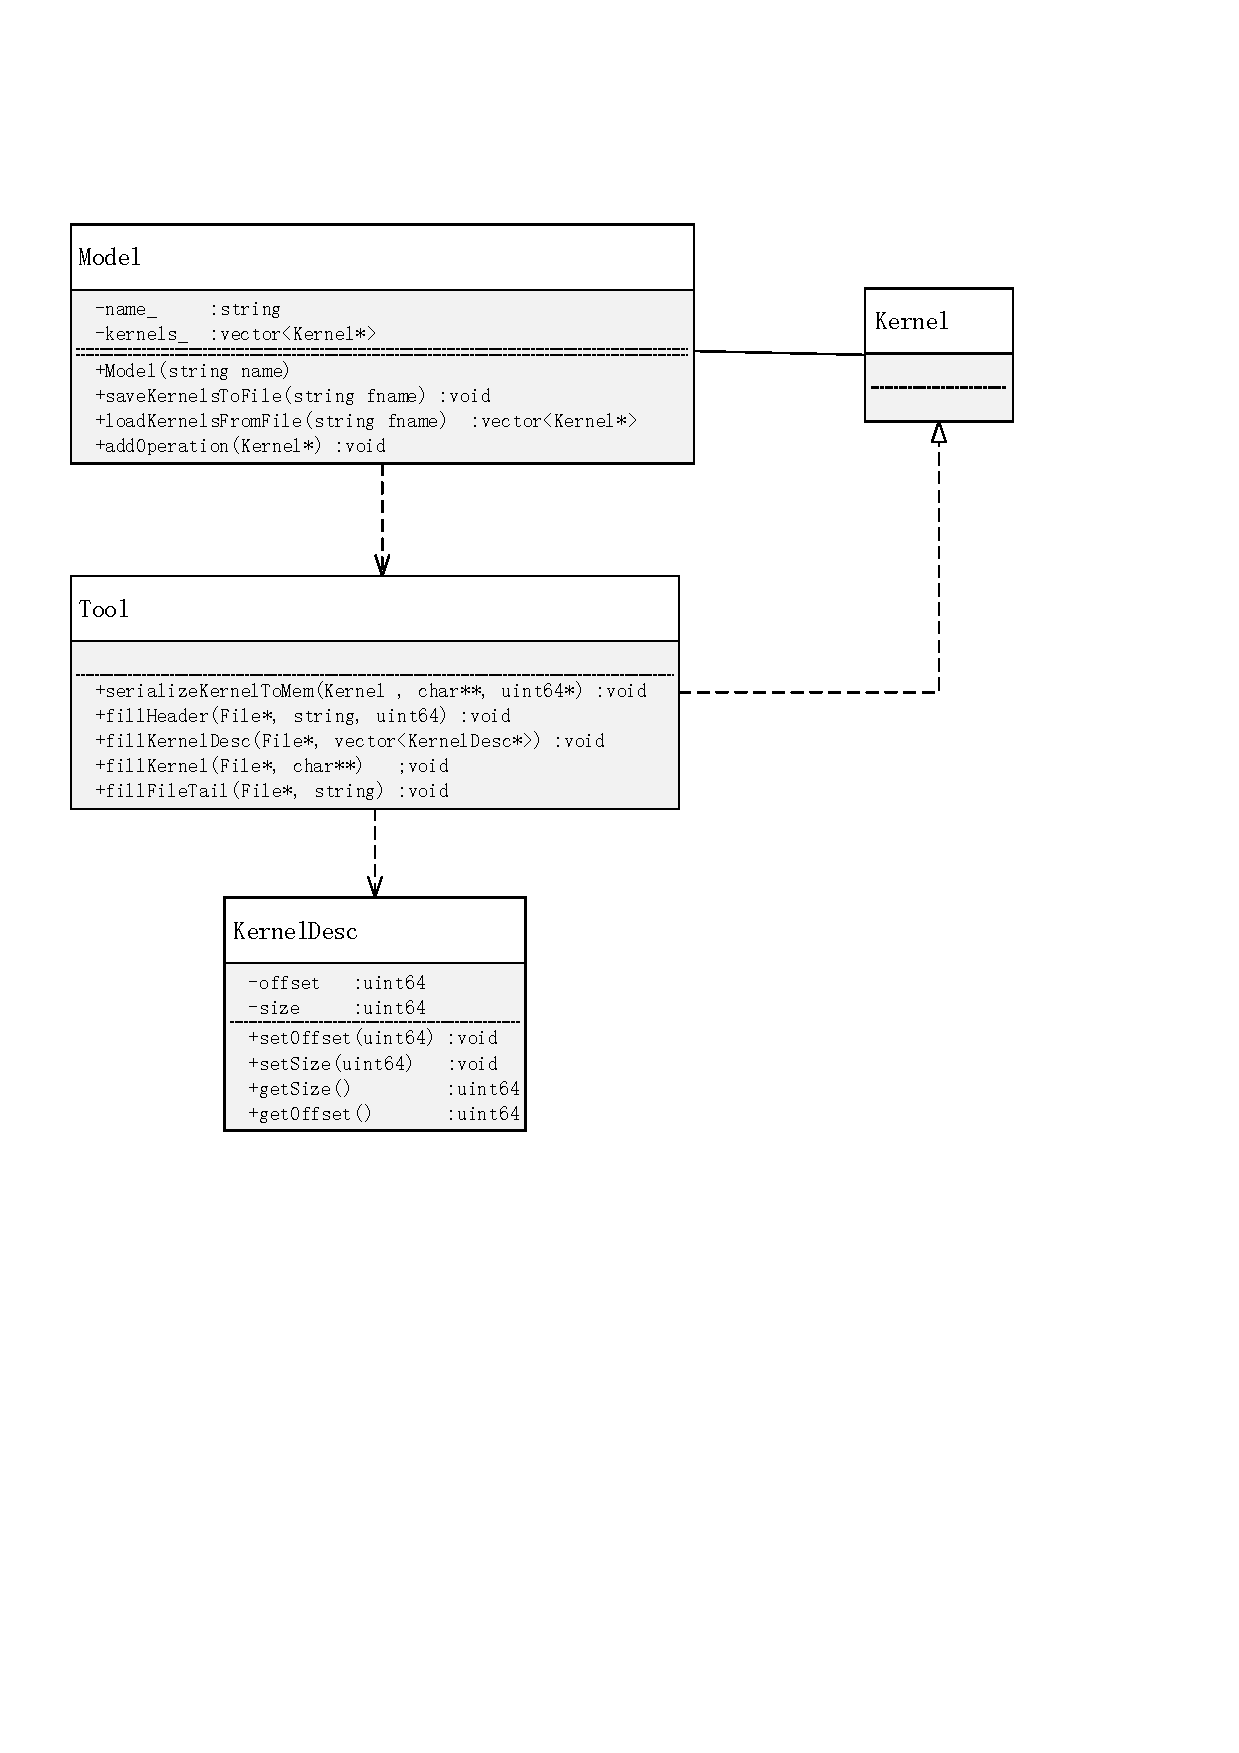
\includegraphics[width=0.5\textwidth]{load_cache_class.pdf}
  \caption{指令保存和加载模块类图}
  \label{fig:load-cache-class}
\end{figure}


该模块的实现主要由4个类组成:Model、Kernel、Tool、KernelDesc。Model作为保存离线模型和加载离线模型的入口;Tool主要实现模型内容的填充。这两个类的主要函数功能见表~\ref{tab:model-tool-function-list}。

\begin{table}[htb]
  \centering\footnotesize
  \caption{Model和Tool主要接口说明}
  \label{tab:model-tool-function-list}
  \begin{tabular}{llll}
    \toprule
    类名        & 函数名     & 功能      & 说明            \\
    \midrule
    Model      & saveKernelsToFile    & 将多个kernel保存到离线文件中 &  \\
               & loadKernelsFromFile  & 从离线文件中加载kernel &    \\
               & addOperation         &向kernels\_中添加kernel & \\
    \midrule
    Tool       & fillKernelDesc & 填充离线模型文件目录部分 & \\
               & fillKernel   & 填充离线模型文件中kernel的内容 & \\
               & fillFileTail & 填充离线模型文件的结尾  & 填入文件前面所有\\
                                                    &&&内容对应的MD5码 \\
               & fillHeader & 填充离线模型文件头 & 传入模型名称和需要    \\
                                                &&&保存的kernel数量\\
               & serializeKernelToMem & 将kernel序列化后 & 传入需要系列化的kernel,\\
                                      &&保存到内存中     & 返回序列化后的字符串地 \\
                                                       &&&址和返回序列化后占用 \\
                                                       &&&空间大小  \\
               
    \bottomrule
  \end{tabular}
\end{table}


在指令缓存的过程中离线模型的文件名,模型名,文件标识符,校验码等信息由程序自动生成,对用户不可见。文件名和模型名都根据之前生成的信息摘要编码组成。文件名=环境信息编码+结构信息编码+权值信息编码,模型名=结构信息编码+权值信息编码,结构如图~\ref{fig:model-name-struct}所示。


\begin{figure}[htb]
  \centering
  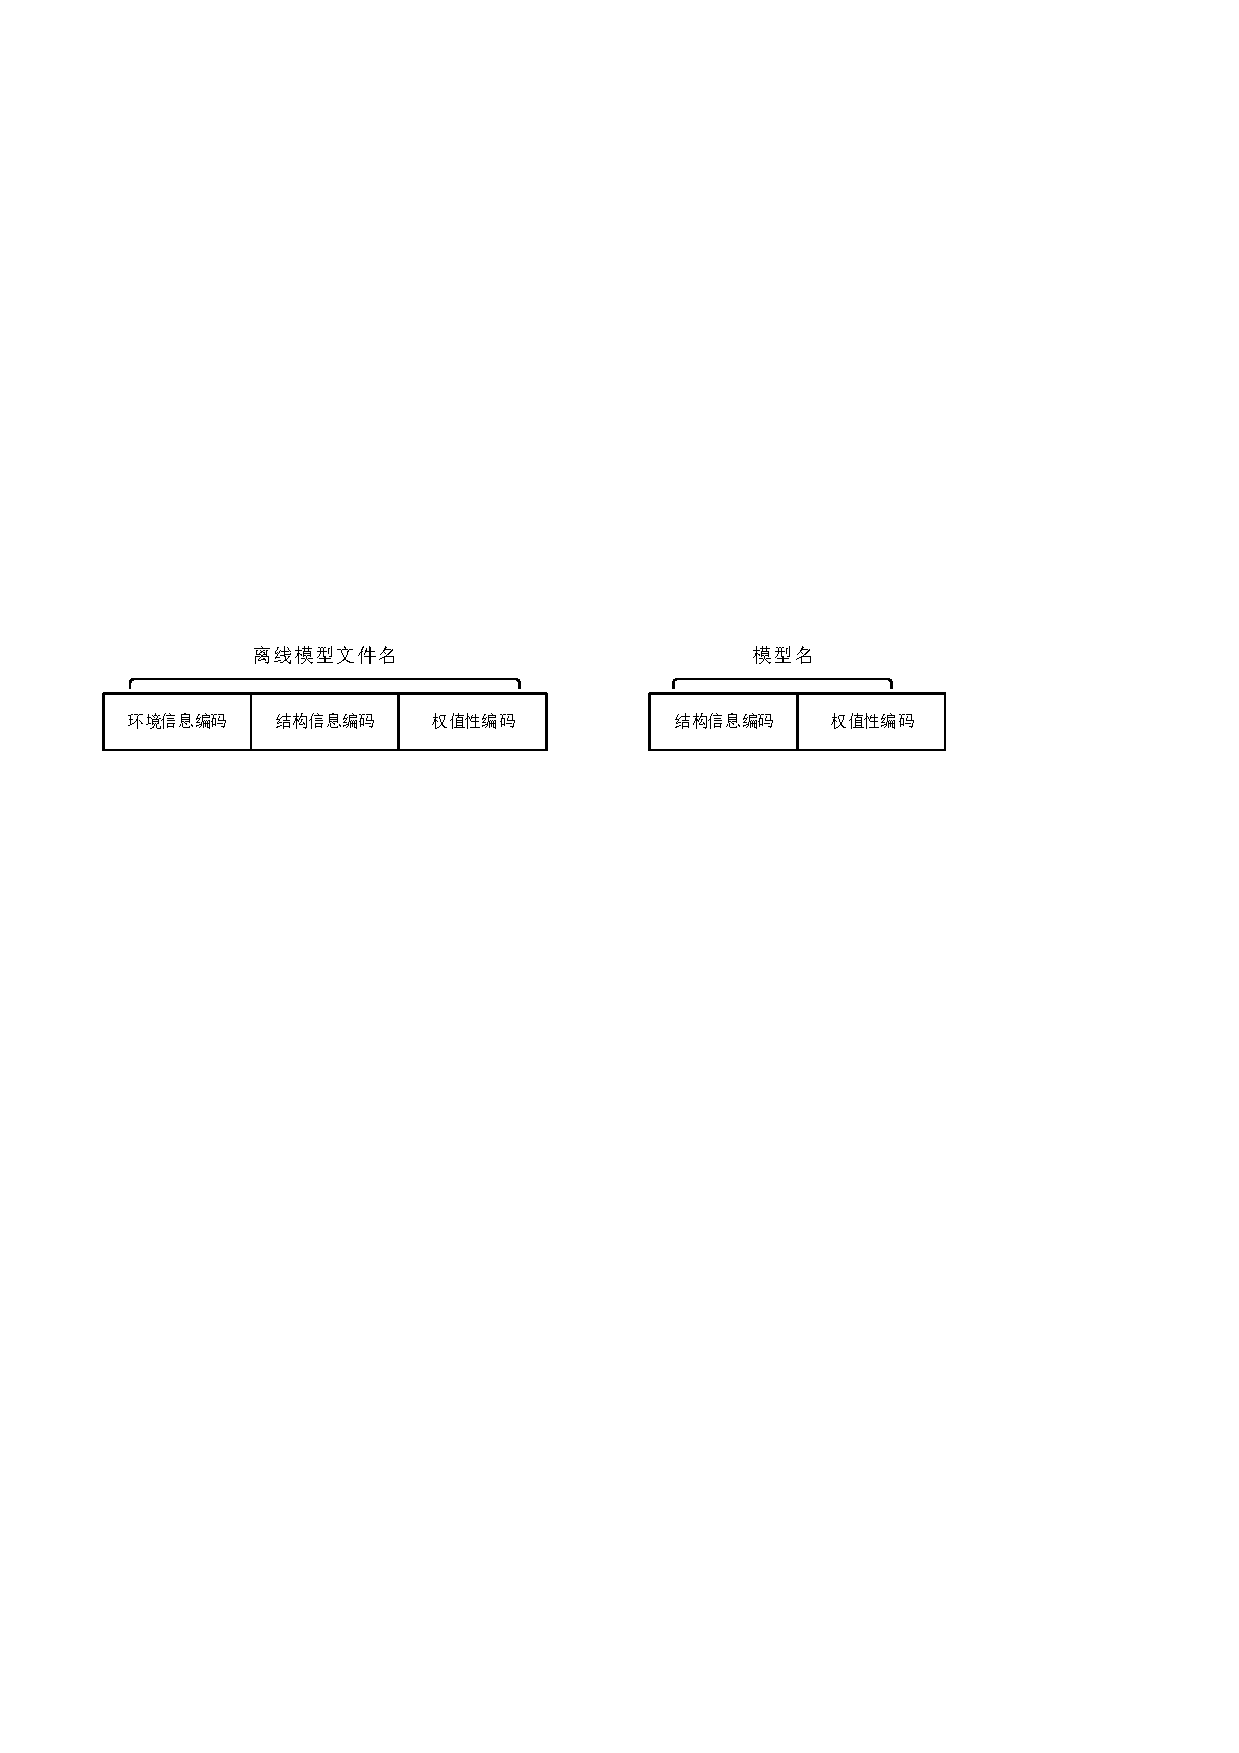
\includegraphics[width=0.8\textwidth]{model_name_struct.pdf}
  \caption{文件名和模型名组成示意图}
  \label{fig:model-name-struct}
\end{figure}

Kernel序列化后的内容就是一个字符串,占用存储空间大小和字符串中字符的数量相关。保存指令通过函数saveKernelsToFile实现,流程如图~\ref{fig:kernel-process}-(a)所示。

\begin{figure}[htb]
  \centering
  \subfigure[保存流程图]{
  \label{fig:save-kernel-process}
  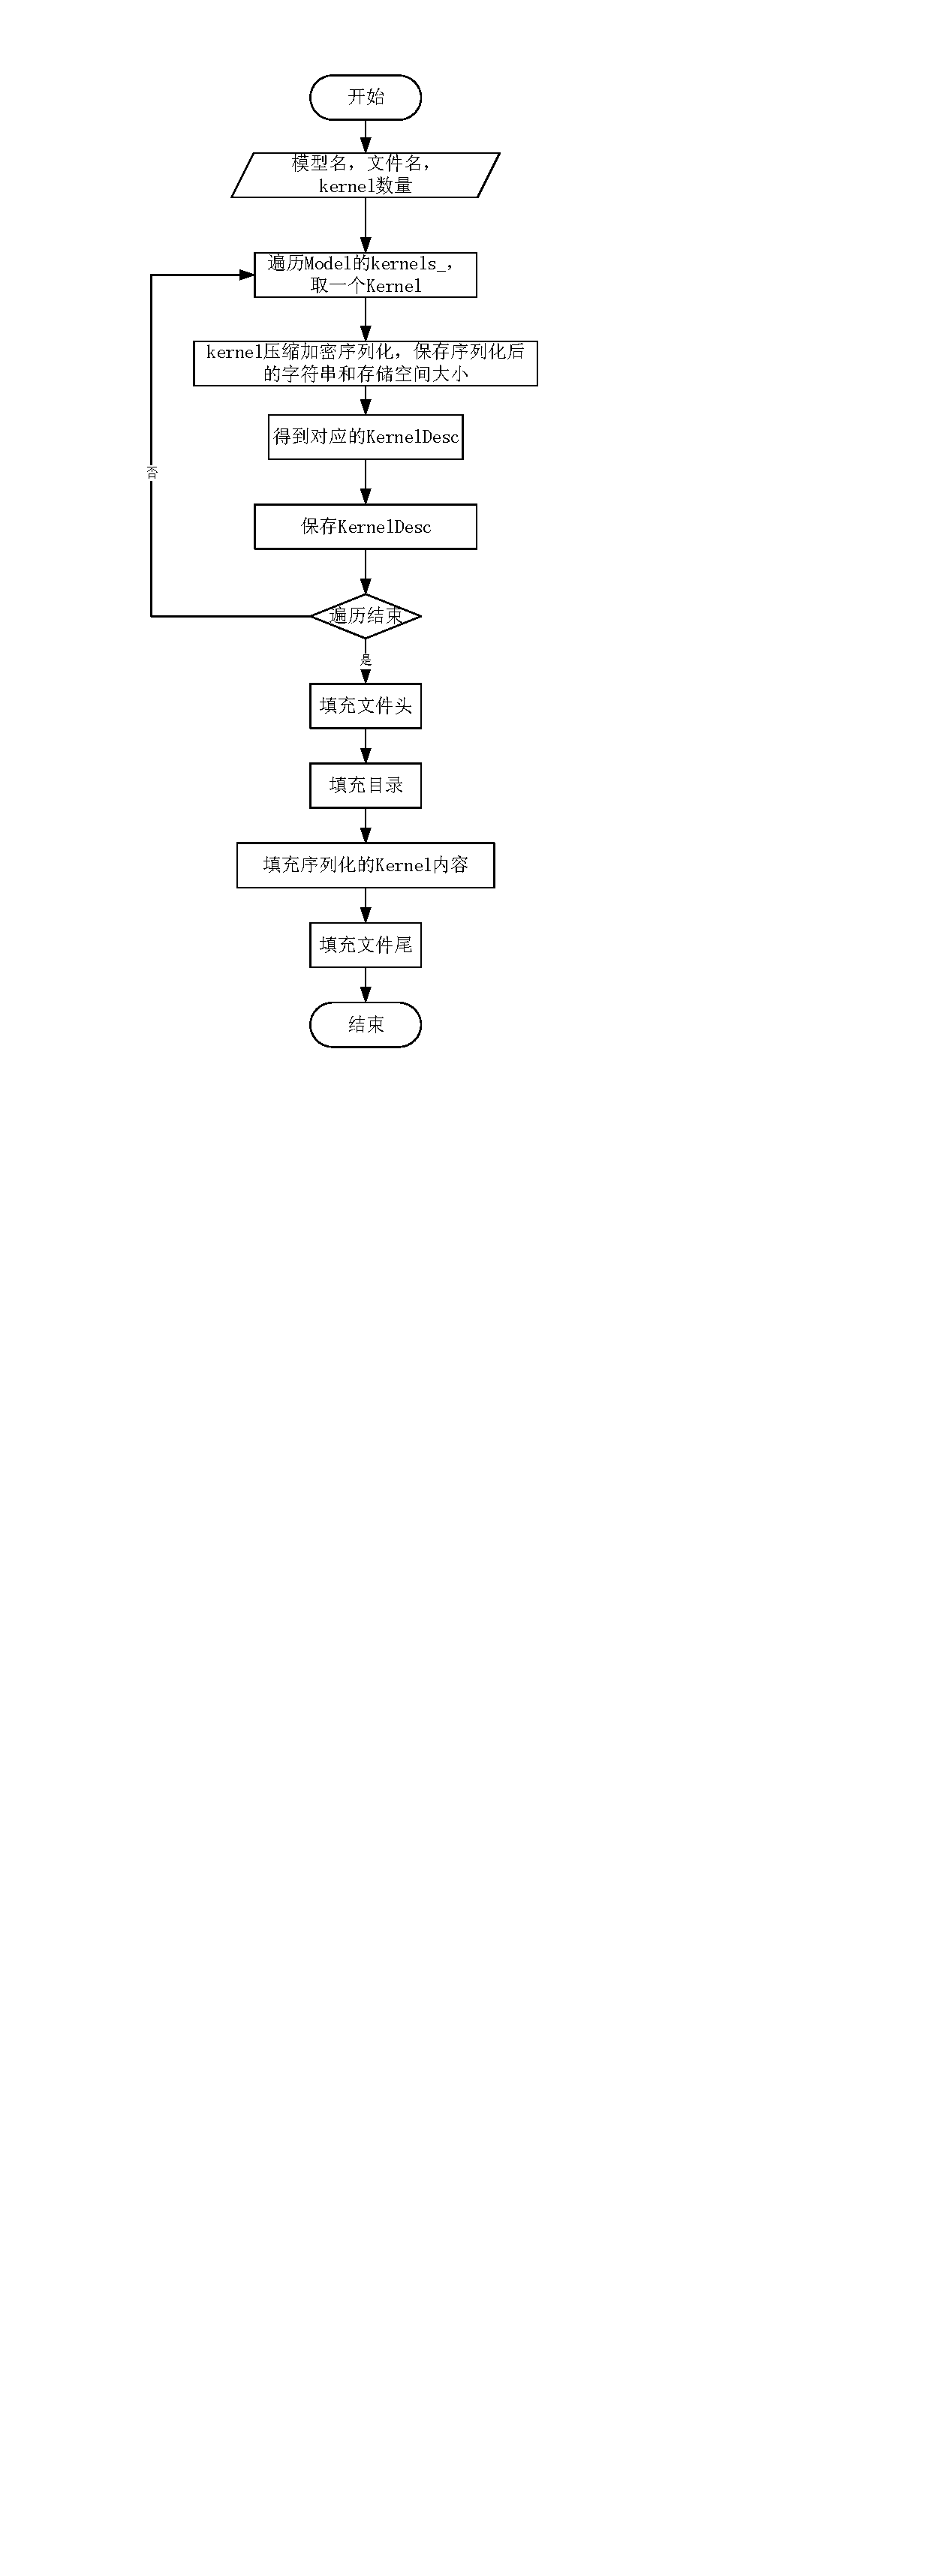
\includegraphics[width=0.45\textwidth]{save_kernel_process.pdf}
  }
  \subfigure[加载流程图]{
  \label{fig:load-kernel-process}
  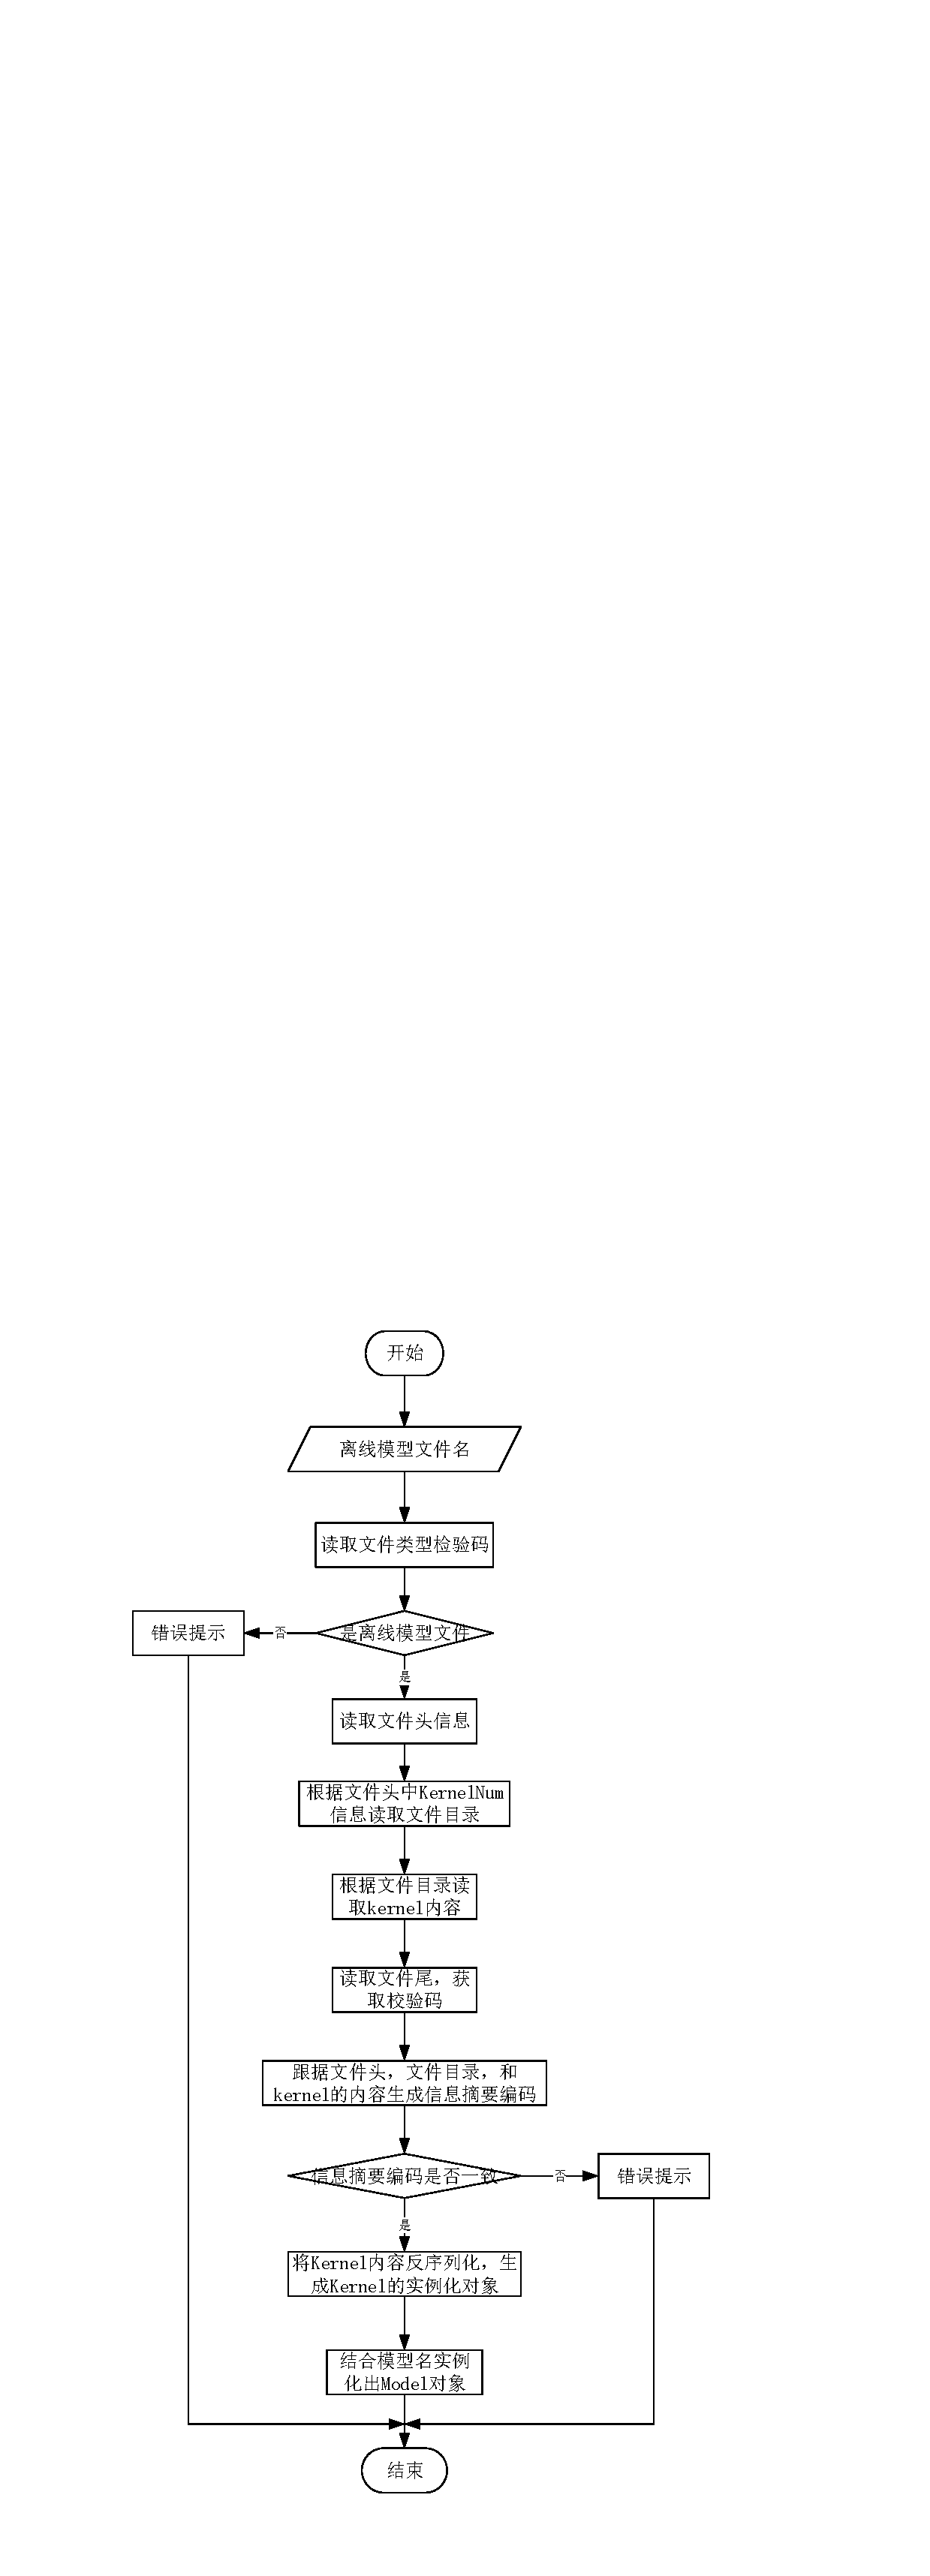
\includegraphics[width=0.4\textwidth]{load_kernel_process.pdf}
  }
  \caption{kernel保存和加载流程图}
  \label{fig:kernel-process}
\end{figure}

保存指令的步骤如下:
\begin{enumerate}
  \item 拿到Model中所有的Kernel
  \item 对每一个Kernel按一定压缩和加密算法进行压缩和加密,得到二级模型(序列化后的字符串)和占用存储空间大小,并用两个数组分别保存;
  \item 根据二级模型大小和偏移,生成对应的KernelDesc并保存到数组中。
  \item 根据二级模型总大小,文件头大小,文件尾大小,目录大小计算出模型文件总大小,将文件总大小、模型数量、模型名、校验码,版本号等文件头信息写入文件。
  \item 遍历保存KernelDesc的数组,将offset和size信息依次写入文件,完成文件目录的填充;
  \item 遍历保存二级模型内容和大小的数组,结合二级模型的内容依次写入文件中,完成文件模型内容的填充
  \item 根据文件头,文件目录和文件模型的内容生成一个信息摘要编码,写入到文件最后,完成文件尾的填充
\end{enumerate}
加载指令是保存指令的逆过程,通过函数loadKernelFromFile完成,流程如图~\ref{fig:kernel-process}-(b)所示。

加载指令的步骤如下:
\begin{enumerate}
  \item 根据传进来的离线模型文件名打开离线模型文件。
  \item 读取文件中文件类型校验码的内容,判断是否是离线模型文件,如果不是,则给出错误提示信息后退出;如果是,则继续进行下一步。
  \item 读取固定大小的文件头内容。
  \item 根据文件头中模型的数量读取文件目录的内容。
  \item 根据文件目录的内容,读取出每个离线模型的内容。
  \item 最后读取文件尾的校验码。
  \item 根据文件头,目录,离线模型的具体内容生成新的信息摘要编码,与文件尾保存的信息摘要编码比较,如果不一致,说明文件损坏,给出提示后退出;如果一致,说明文件完好,继续执行下一步。
  \item 发序列化离线模型的内容,生成Kernel的实例化对象。
  \item 结合模型名,生成Model的实例化对象。
\end{enumerate}
生成kernel的实例化对象之后将kernel送给模型执行器,继续执行kernel的计算过程。

\section {权值替换模块设计与实现}
在神经网络应用中,神经网络结构相同,权值(为了方便起见,这里将filter和bias统称为权值)不同的情况经常发生,为了尽可能的避免神经网络的重复编译(编译阶段耗费大量的时间)。当遇到结构相同,权值数据不同的情况下,我们可以通过权值替换的手段来避免二次编译。

权值替换的原理就是拿一份结构相同的已经编译好的离线模型文件,替换掉其中的权值数据。由于网络模型结构相同,替换数据之后和新编译生成的指令完全一样,所以执行结果不会产生差异。

实现过程中涉及到的类及其方法如图~\ref{fig:weight-replace-class}所示。

\begin{figure}[htb]
  \centering
  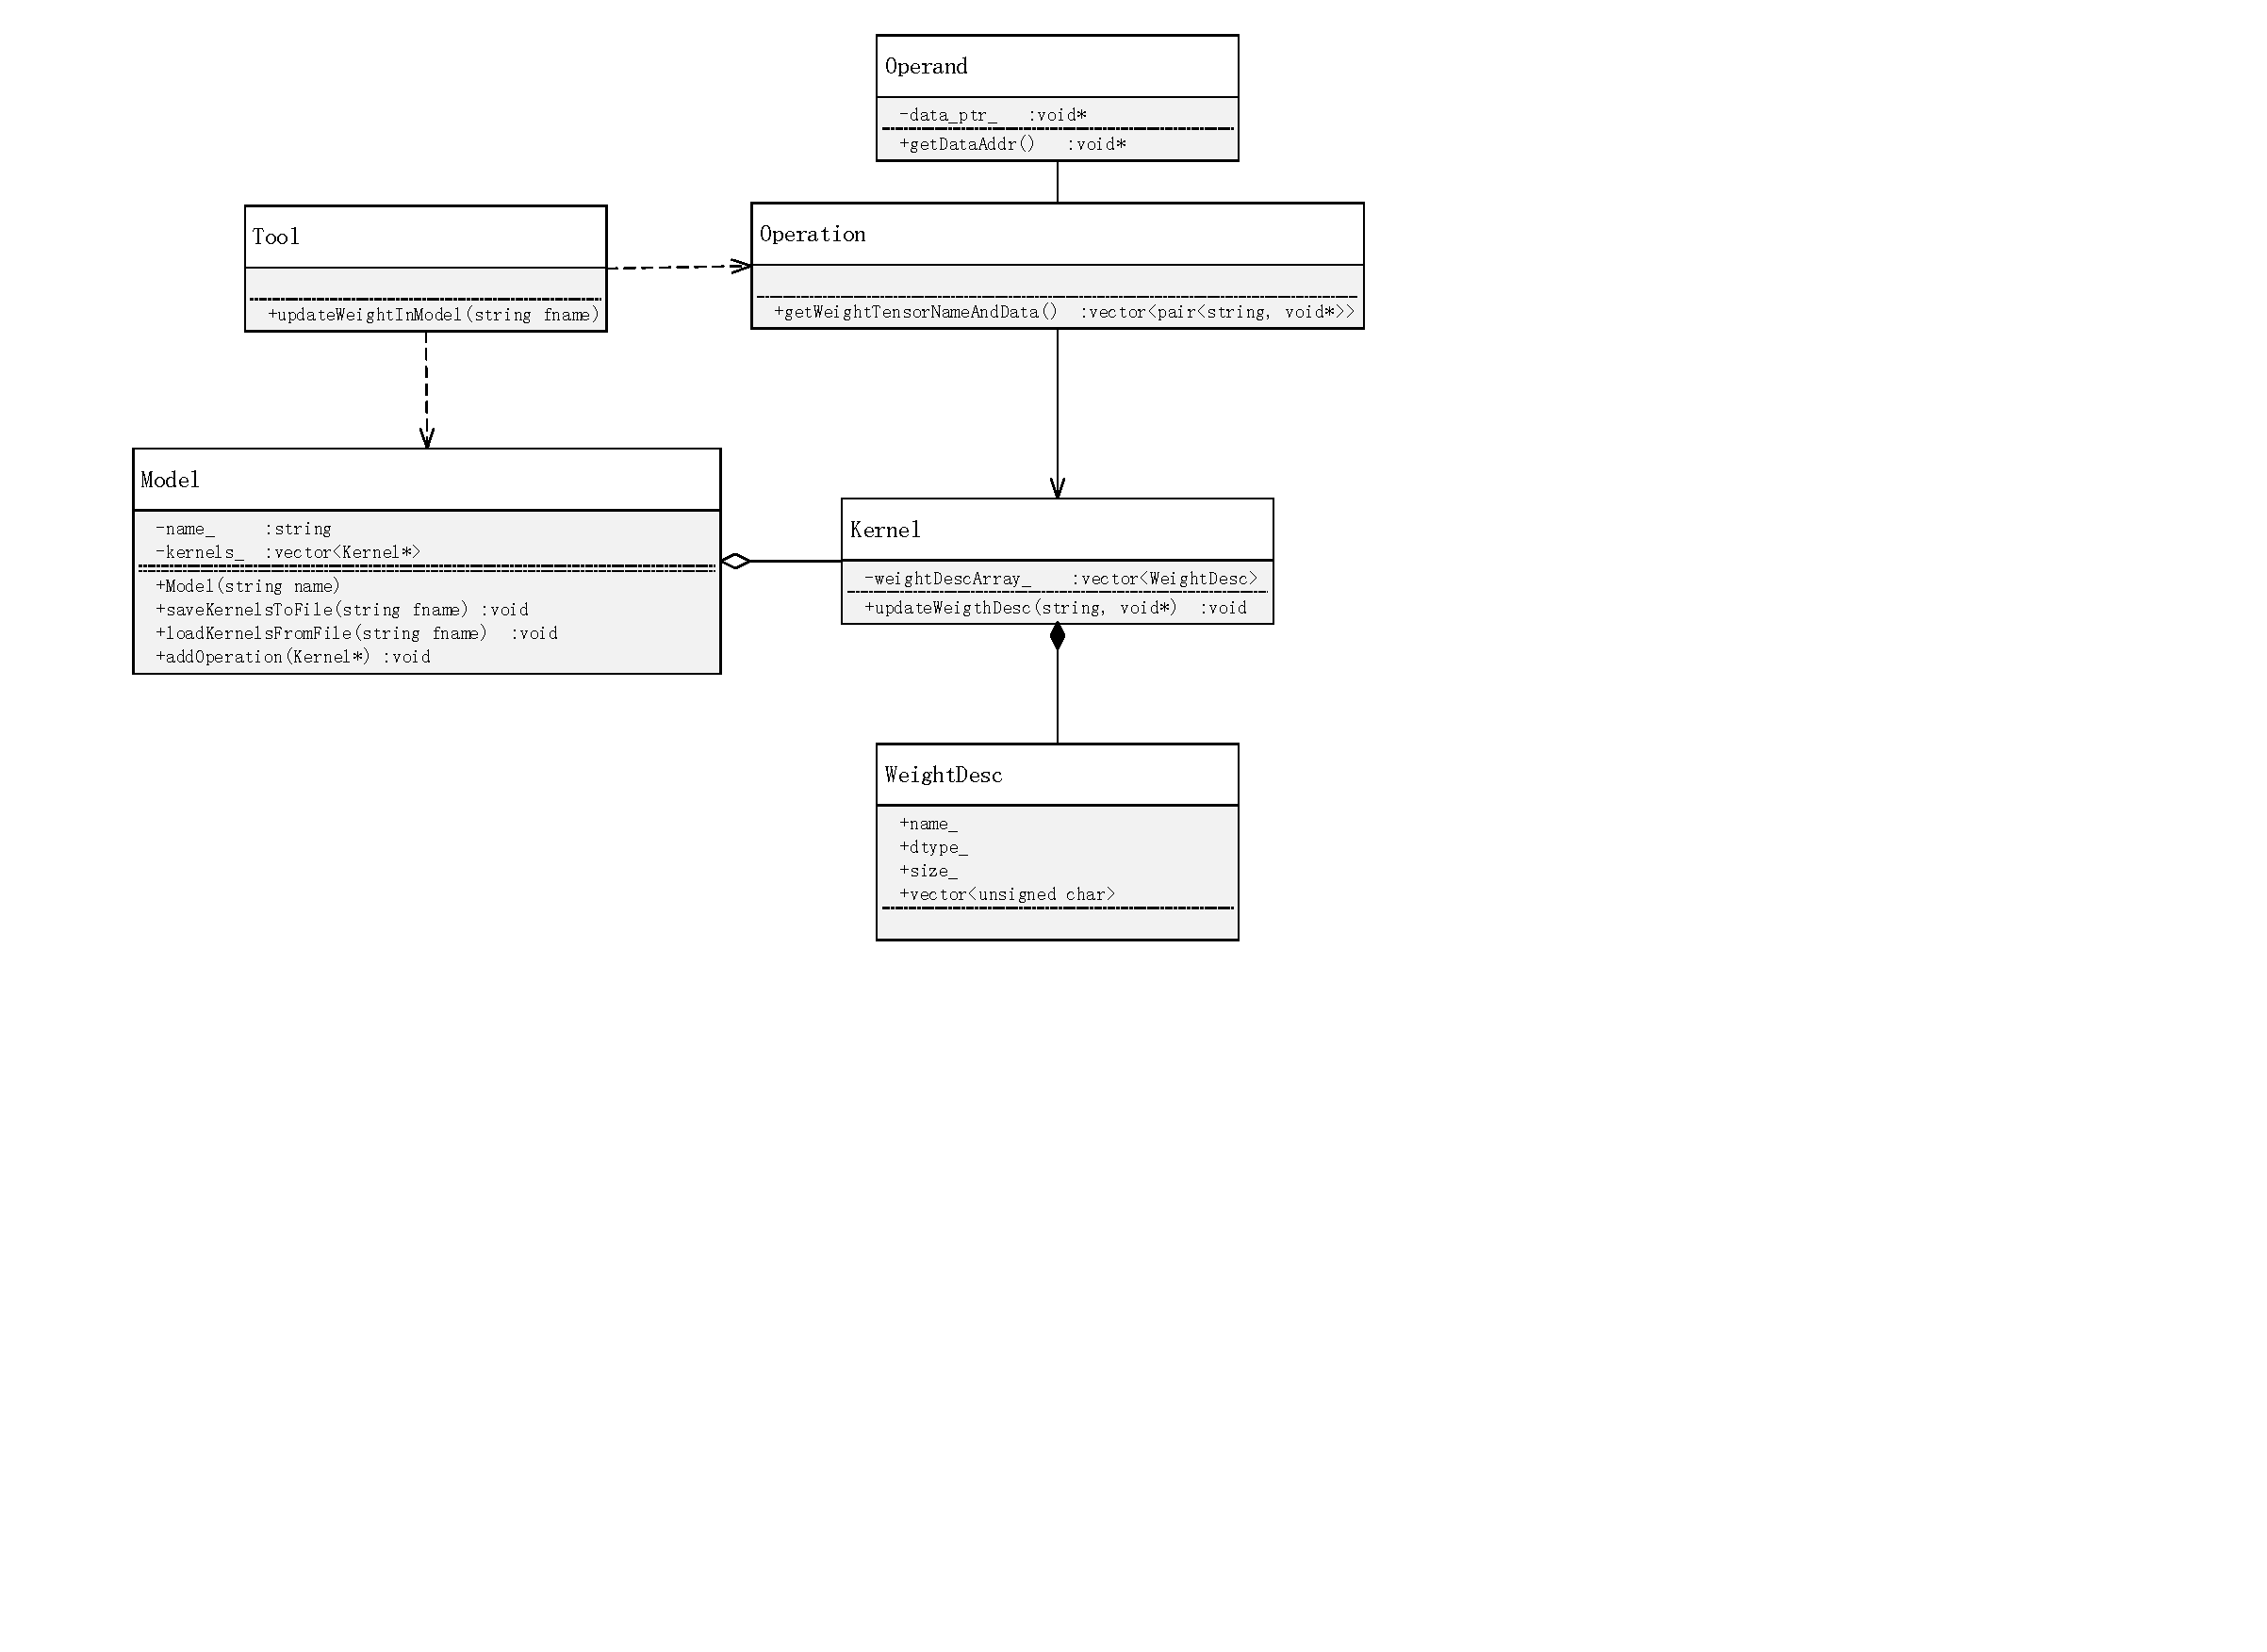
\includegraphics[width=0.8\textwidth]{weight_replace_class.pdf}
  \caption{权值替换模块类图}
  \label{fig:weight-replace-class}
\end{figure}

其中WeightDesc用于保存权值信息,包括对应的Tensor名称、数据类型、数据个数、和实际数值,为了方便存储和读取各种类型的数据,用unsigned char类型存储实际数据,取值的时候根据数据类型,将unsigned char类型转换为对应的数据。主要函数说明见表~\ref{tab:weight-replace-function-list}。

\begin{table}[htb]
  \centering\small
  \caption{权值替换模块主要函数说明}
  \label{tab:weight-replace-function-list}
  \begin{tabular}{lll}
    \toprule
    函数名        & 功能     & 函数说明                 \\
    \midrule
    Tool:updateWeightInModel  & 更新指定离线模型 &将多个kernel保存到 \\
                              &文件中的权值数据   离线文件中\\
    \midrule
    Operand:getDataAddr & 获取Tensor绑定 &如果没有绑定数据,\\
                        &数据的地址   & 则返回默认值nullptr  \\
    \midrule
    Operation: & 获取操作中所有Filter和Bias &如果是融合操作,会返 \\
    getWeightTensorNameAndData  & 类型的Tensor的名称 & 回图中所有操作的Filter\\
                      &和绑定的数据地址 &和Bias类型Tensor的 \\
                      &                &名称和绑定的数据地址 \\
    \midrule
    Kernel: updateWeightDesc  & 更新kernel中指定 & 第一个参数是Tensor名 \\
                              & Tensor绑定的数据 & 称,第二个参数新数据地址 \\
    \bottomrule
  \end{tabular}
\end{table}

权值替换实现的流程如图~\ref{fig:weight-replace-process}所示。

\begin{figure}[htb]
  \centering
  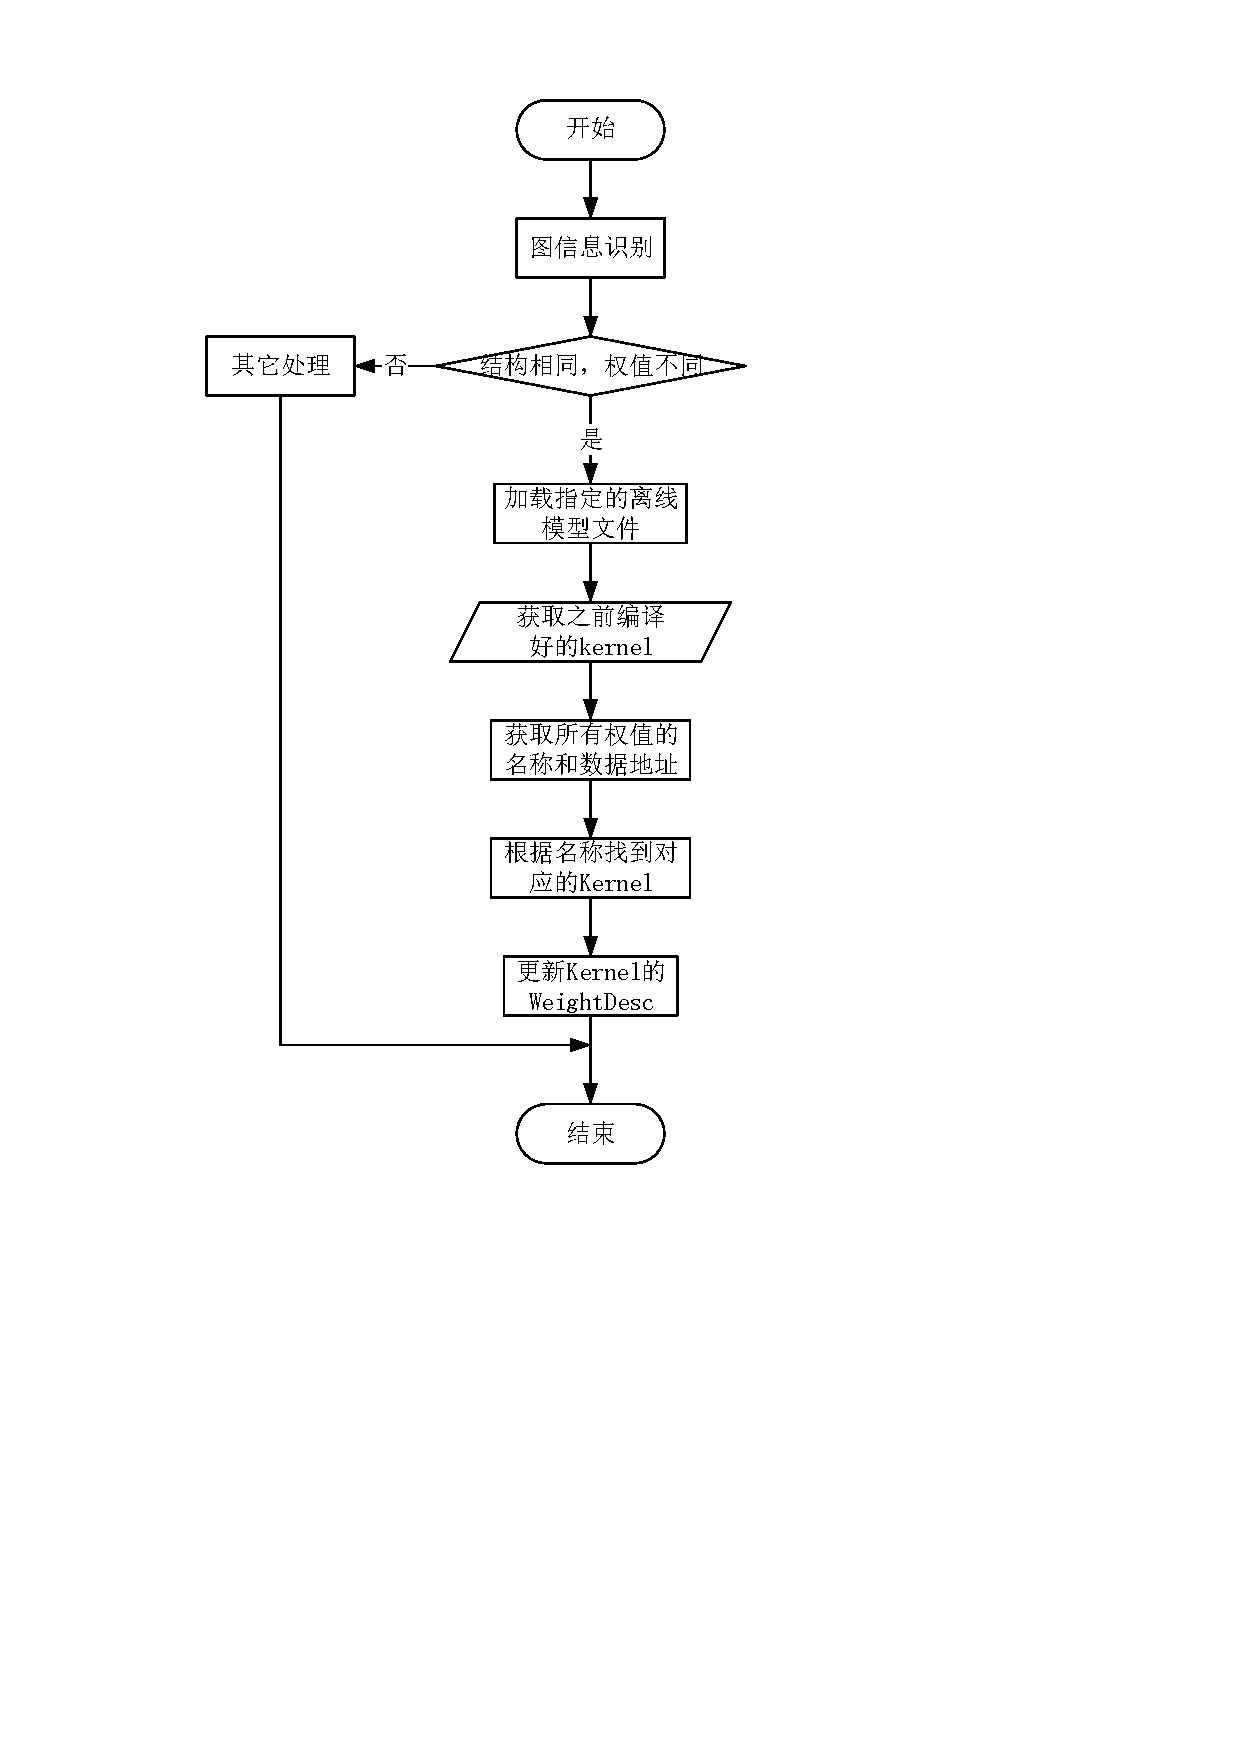
\includegraphics[width=0.3\textwidth]{weight_replace_process.pdf}
  \caption{权值替换模块流程图}
  \label{fig:weight-replace-process}
\end{figure}

如果在图信息识别模块中识别出是结构相同而权值不同的情况则进行权值替换。首先加载一份结构相同的离线模型文件,解析文件,生成对应的kernel对象;然后查找出所有绑定权值信息的Tensor的名称和绑定的数据地址;之后根据tensor的名称查找出对应的kernel对象,更新kernel中对应Tensor的数据。

权值信息更新完毕后,将kernel送入模型执行器,并保存一份新的离线模型文件,更新权值信息缓存表。

\section {指令替换模块设计与实现}

指令替换模块是指令缓存的子功能,当缓存空间不足时进行指令替换,删除旧指令文件,保存新指令文件。
为了支持用户友好性,用环境变量MODEL\_CACHE\_DISABLE来控制是否开启指令缓存,默认值为0,默认情况下开启指令缓存功能,值为1时关闭指令缓存功能;用环境变量MODEL\_CACHE\_MAXSIZE来设定缓存空间大小,只有当MODEL\_CACHE\_DISABLE的值为0时设置该环境变量才有效。当指令缓存关闭时,编译阶段不会执行计算图信息保存、识别,权值替换等流程。

指令替换采用先进先出(First In First Out、FIFO)的原则,符合缓存功能的定义也符合深度学习的使用场景,特别是在训练阶段,为了达到满意的效果,经常需要不断的调整权值信息。此时根据先进先出的原则,可以大概率的编译重复编译。

为了实现指令替换,我们还需要用一个环境变量ACHE\_SIZE\_LEFT来保存当前缓存空间的剩余量。替换流程如图~\ref{fig:cache-replace-process}所示。

\begin{figure}[htb]
  \centering
  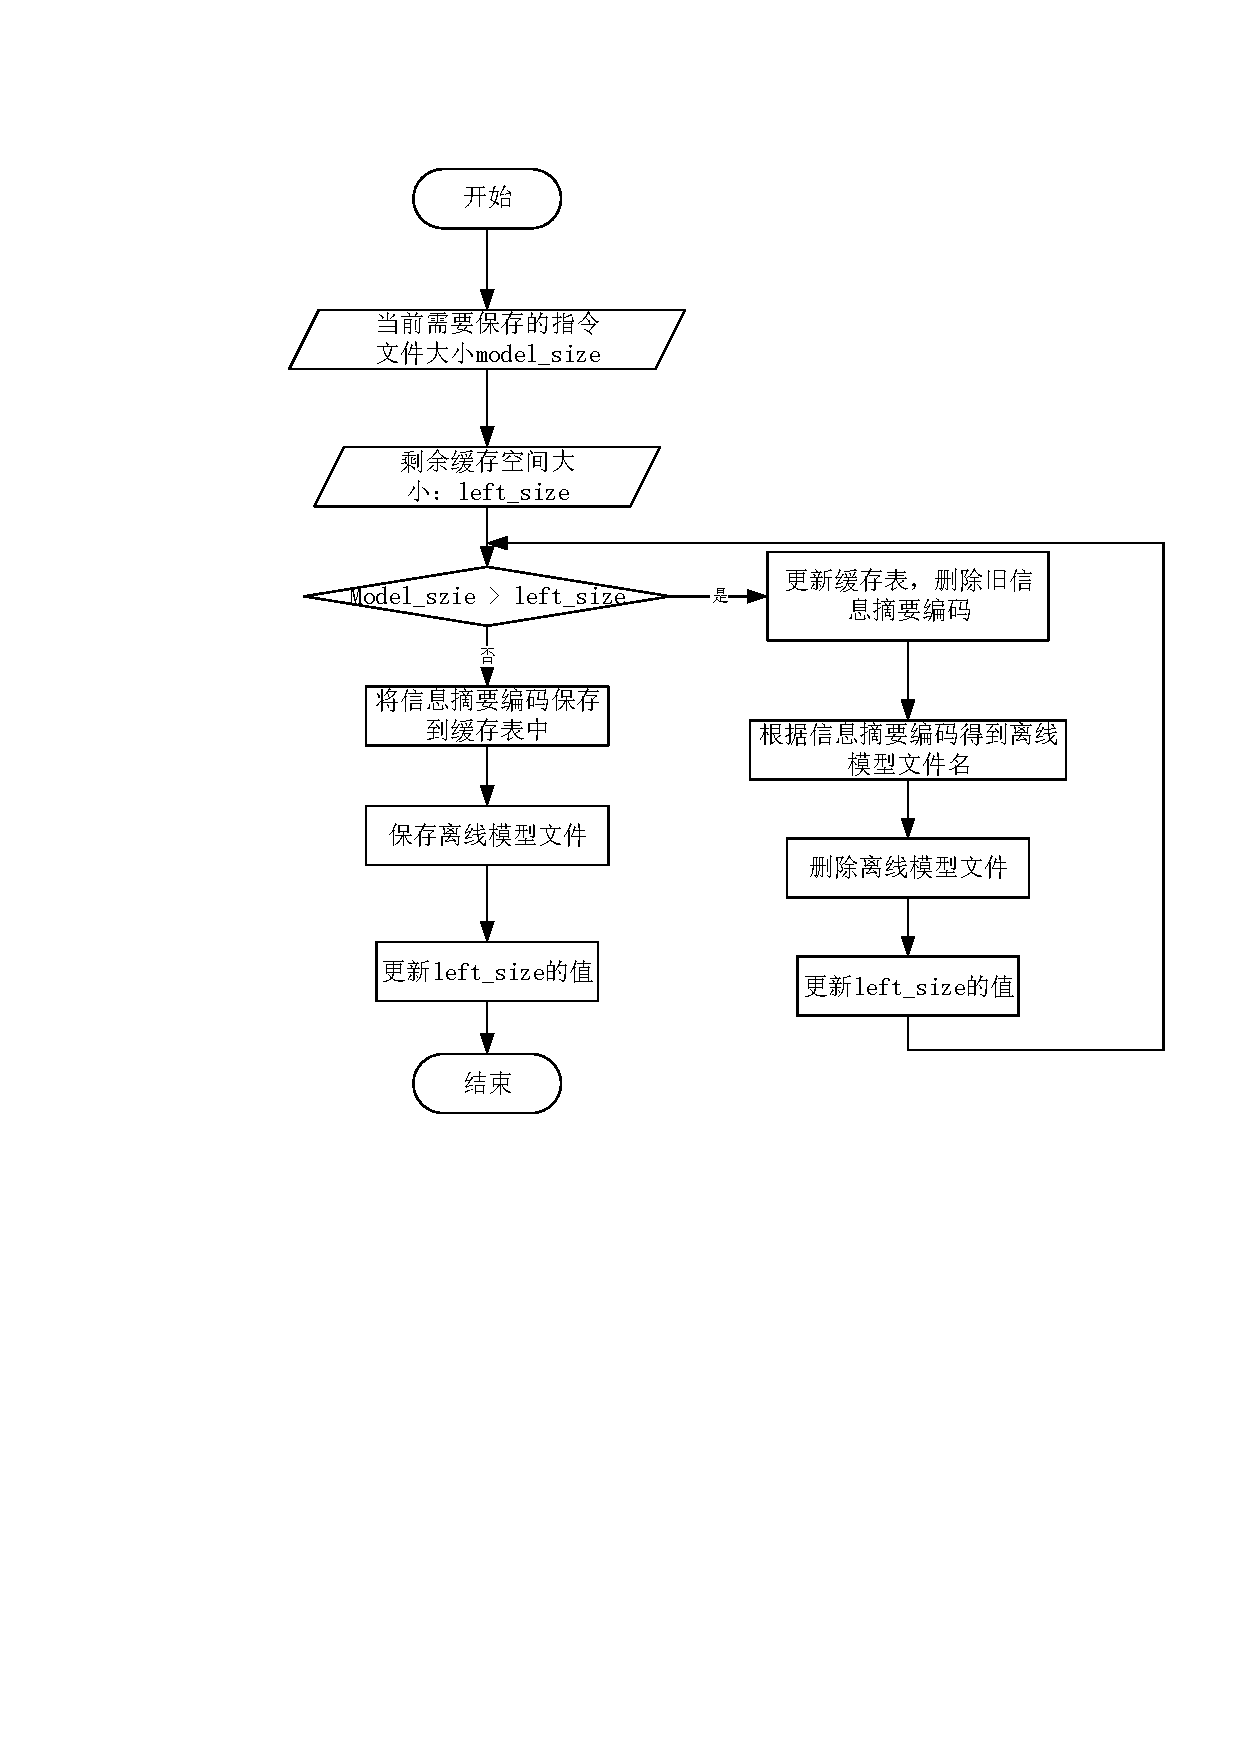
\includegraphics[width=0.6\textwidth]{cache_replace_process.pdf}
  \caption{替换离线模型流程图}
  \label{fig:cache-replace-process}
\end{figure}

首先判断当前缓存的剩余空间是否充足,如果剩余空间充足,则直接更新缓存表,保存新的离线模型文件,更新剩余空间的值即可;如果剩余的空间不充足,则删除最旧的离线模型文件,更新缓存表,更新剩余空间的值,重新比较剩余空间是否满足,如果不满足则继续删除离线文件的过程,直到剩余空间大小满足为止。

\section {权值量化模块设计与实现}
权值量化通过利用低精度的int8类型的数据来表示量化后的float型的数据从而达到模型压缩的目的。事实上,在对精度要求并不是十分苛刻的情况下,量化神经网络不仅能压缩神经网络的空间,更能提高神经网络的推理和训练速度。
为了用户友好性,由用户通过环境变量ENABLE\_QUANTIFY\_MODEL来控制是否开启权值量化。默认值为false,不开启权值量化功能;当环境变量值为true时,开启权值量化功能。类图如~\ref{fig:weight-quant-class}所示。

\begin{figure}[htb]
  \centering
  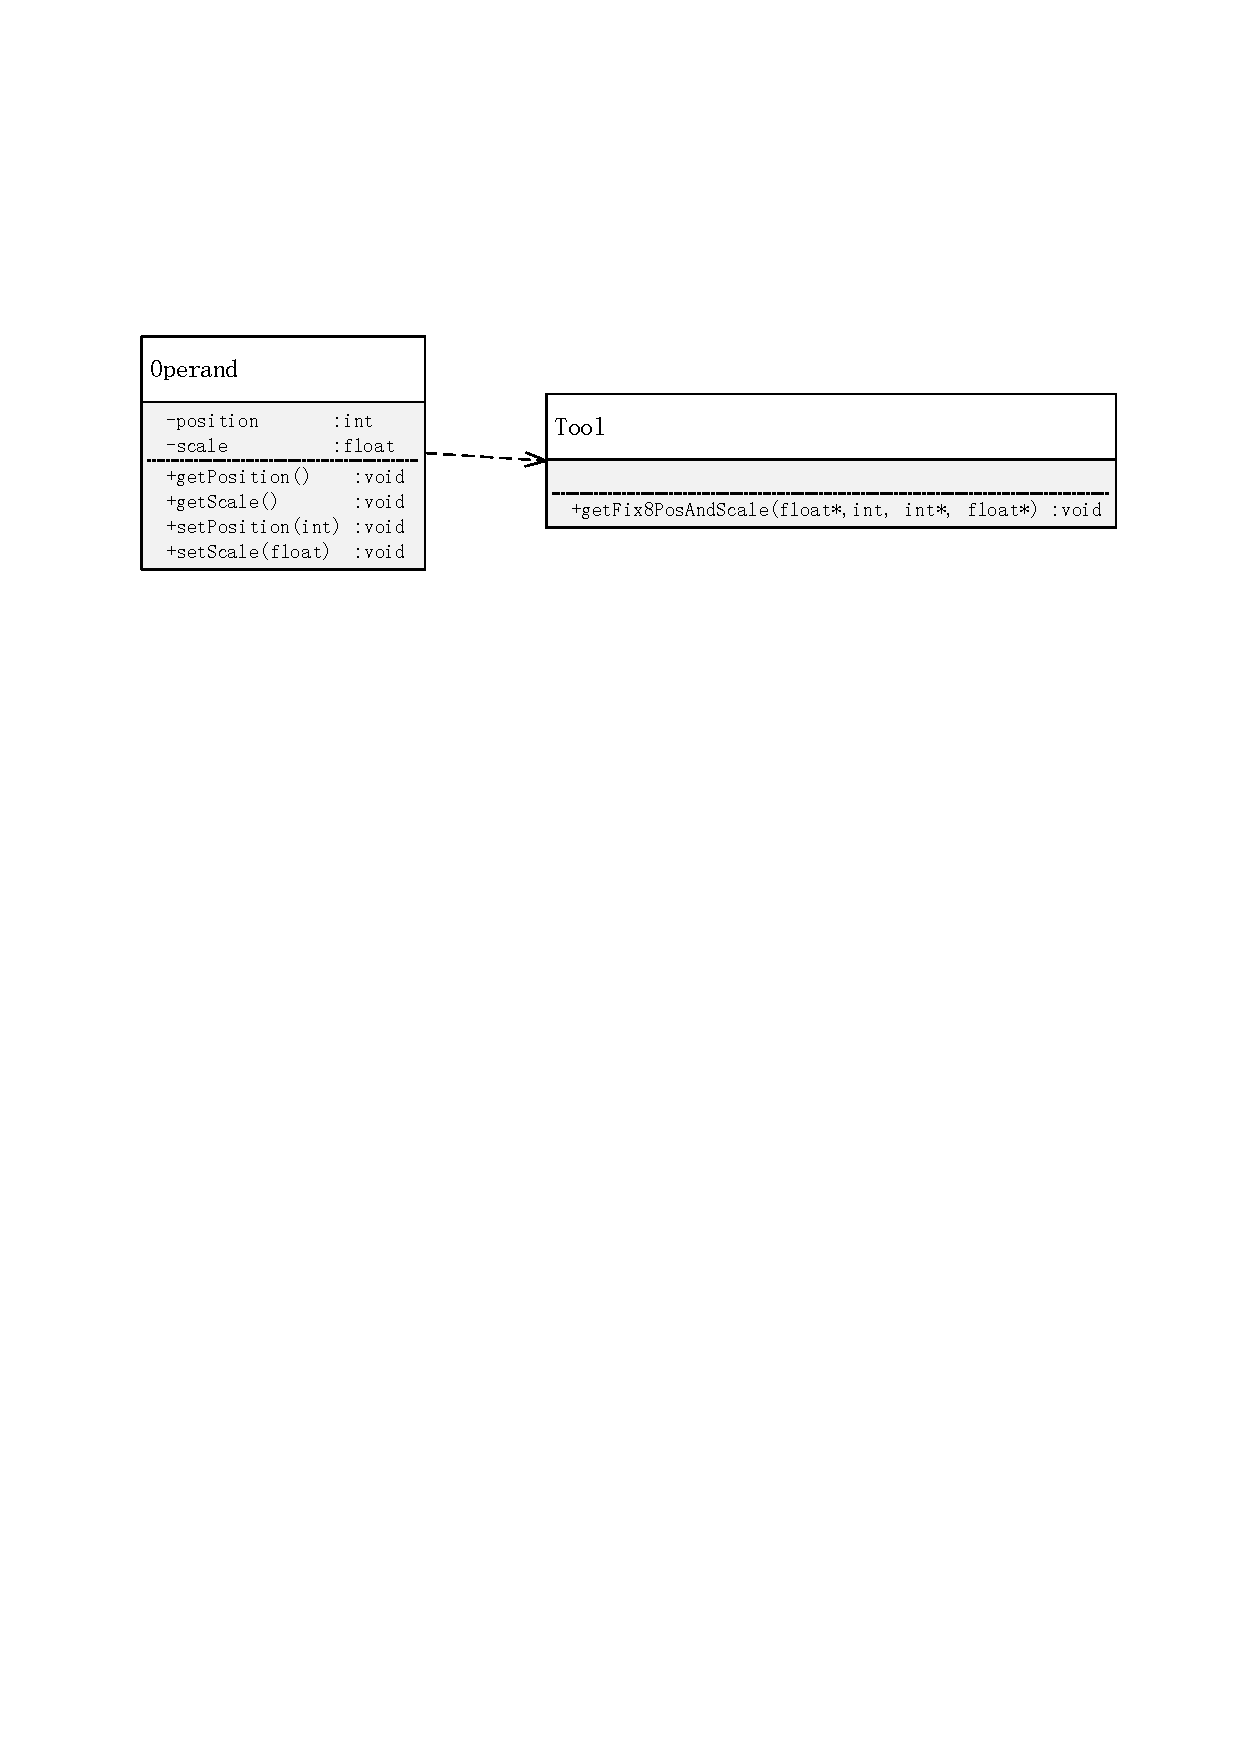
\includegraphics[width=0.9\textwidth]{weight_quant_class.pdf}
  \caption{权值量化模块类图}
  \label{fig:weight-quant-class}
\end{figure}

首先在数据描述的基类Operand中添加position和scale属性,用于保存量化后的参数,position的默认值为0,scale默认值为1,当position和scale的值都等于默认值时,则表示数据没有做量化处理。然后在工具类中添加一个求量化参数的函数getFix8PosAndScale,求出将float型数据量化成int型时的量化参数。函数中第一个参数表示原数据地址,第二个参数表示数据个数,第三个参数用来存返回的position的值,第四个参数用来存返回的scale的值。之后在kernel的WeightDesc中添加相应关于量化的描述信息,其结构如图~\ref{fig:quant-desc}所示。

\begin{figure}[htb]
  \centering
  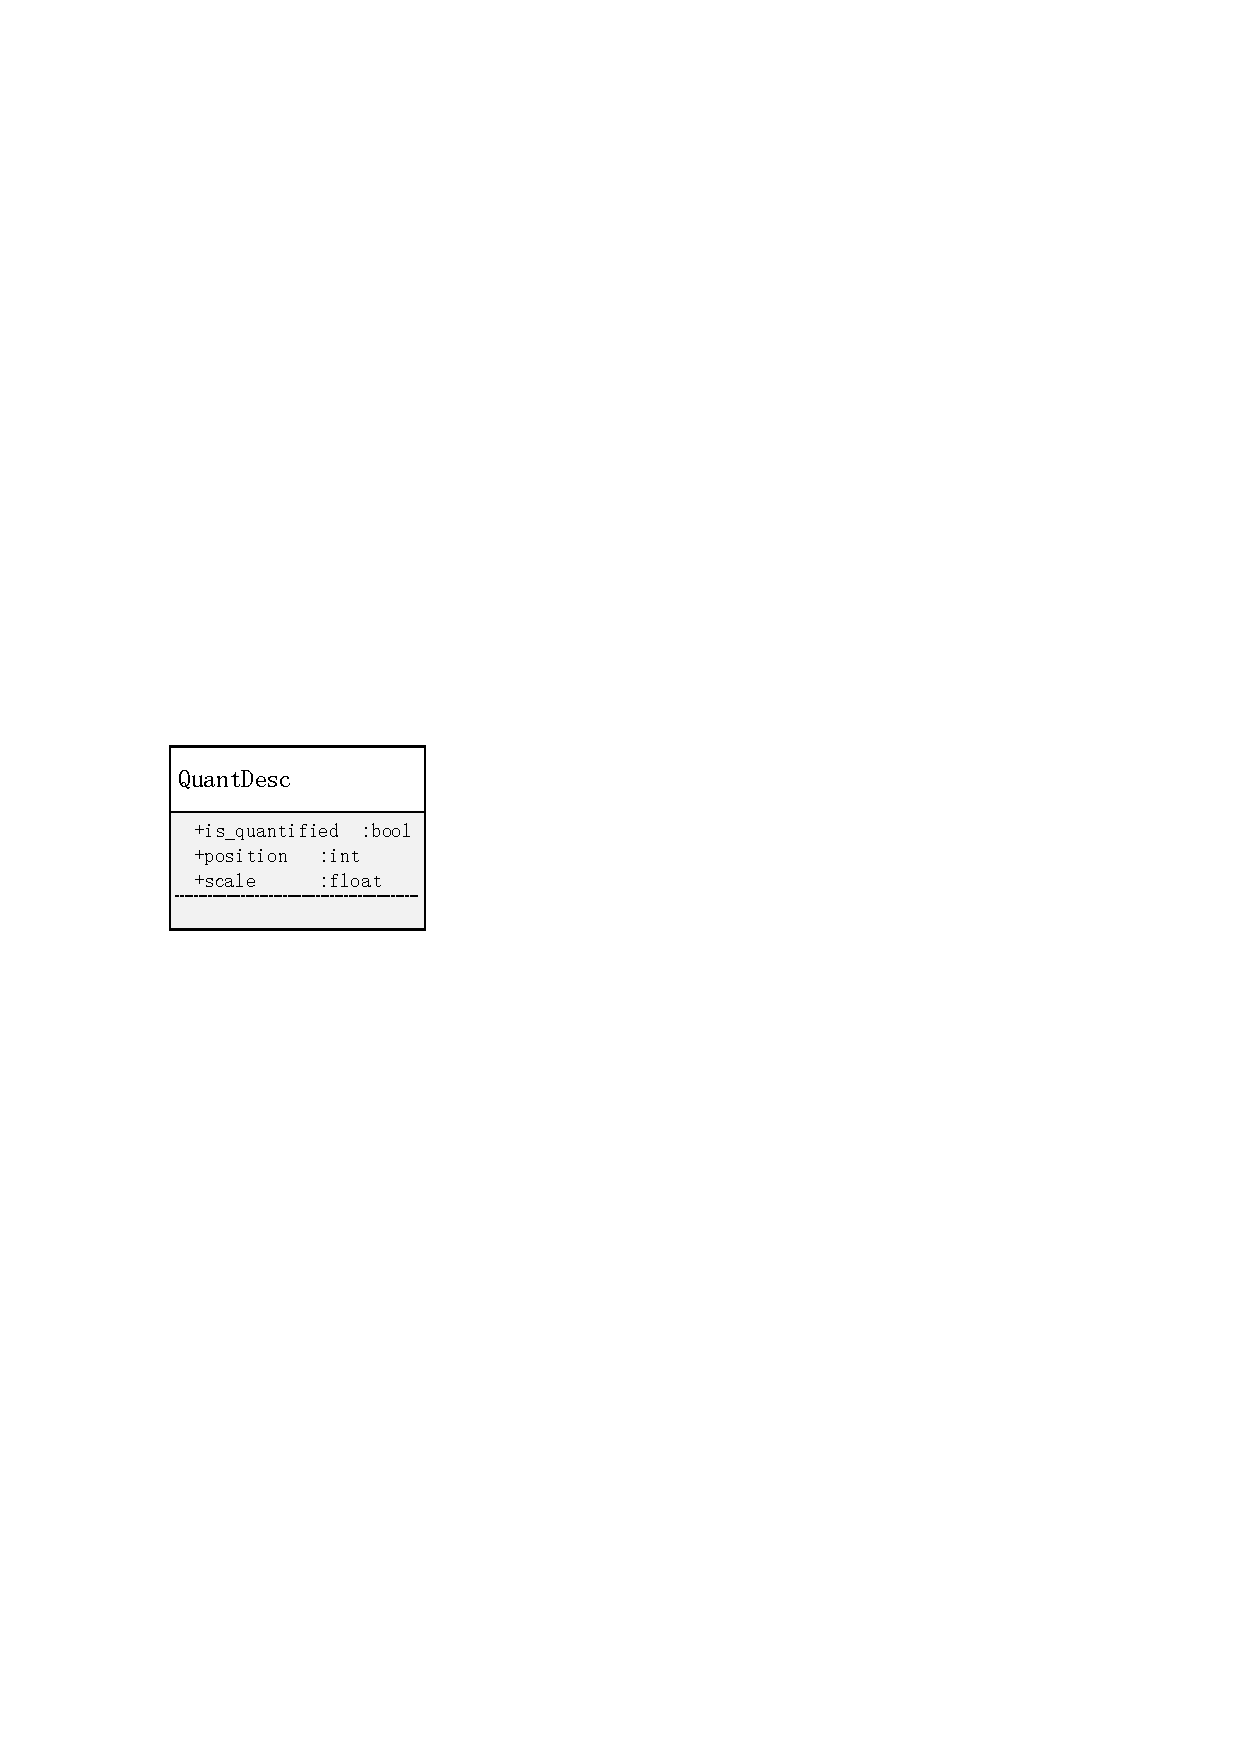
\includegraphics[width=0.4\textwidth]{quant_desc.pdf}
  \caption{量化信息图}
  \label{fig:quant-desc}
\end{figure}

QuantDesc中is\_quantified用来判断数据是否被量化,默认值是false,position和scale用来保存量化参数,默认值分别是0和1.0。
权值量化的过程如图~\ref{fig:weight-quant-process}所示。

\begin{figure}[htb]
  \centering
  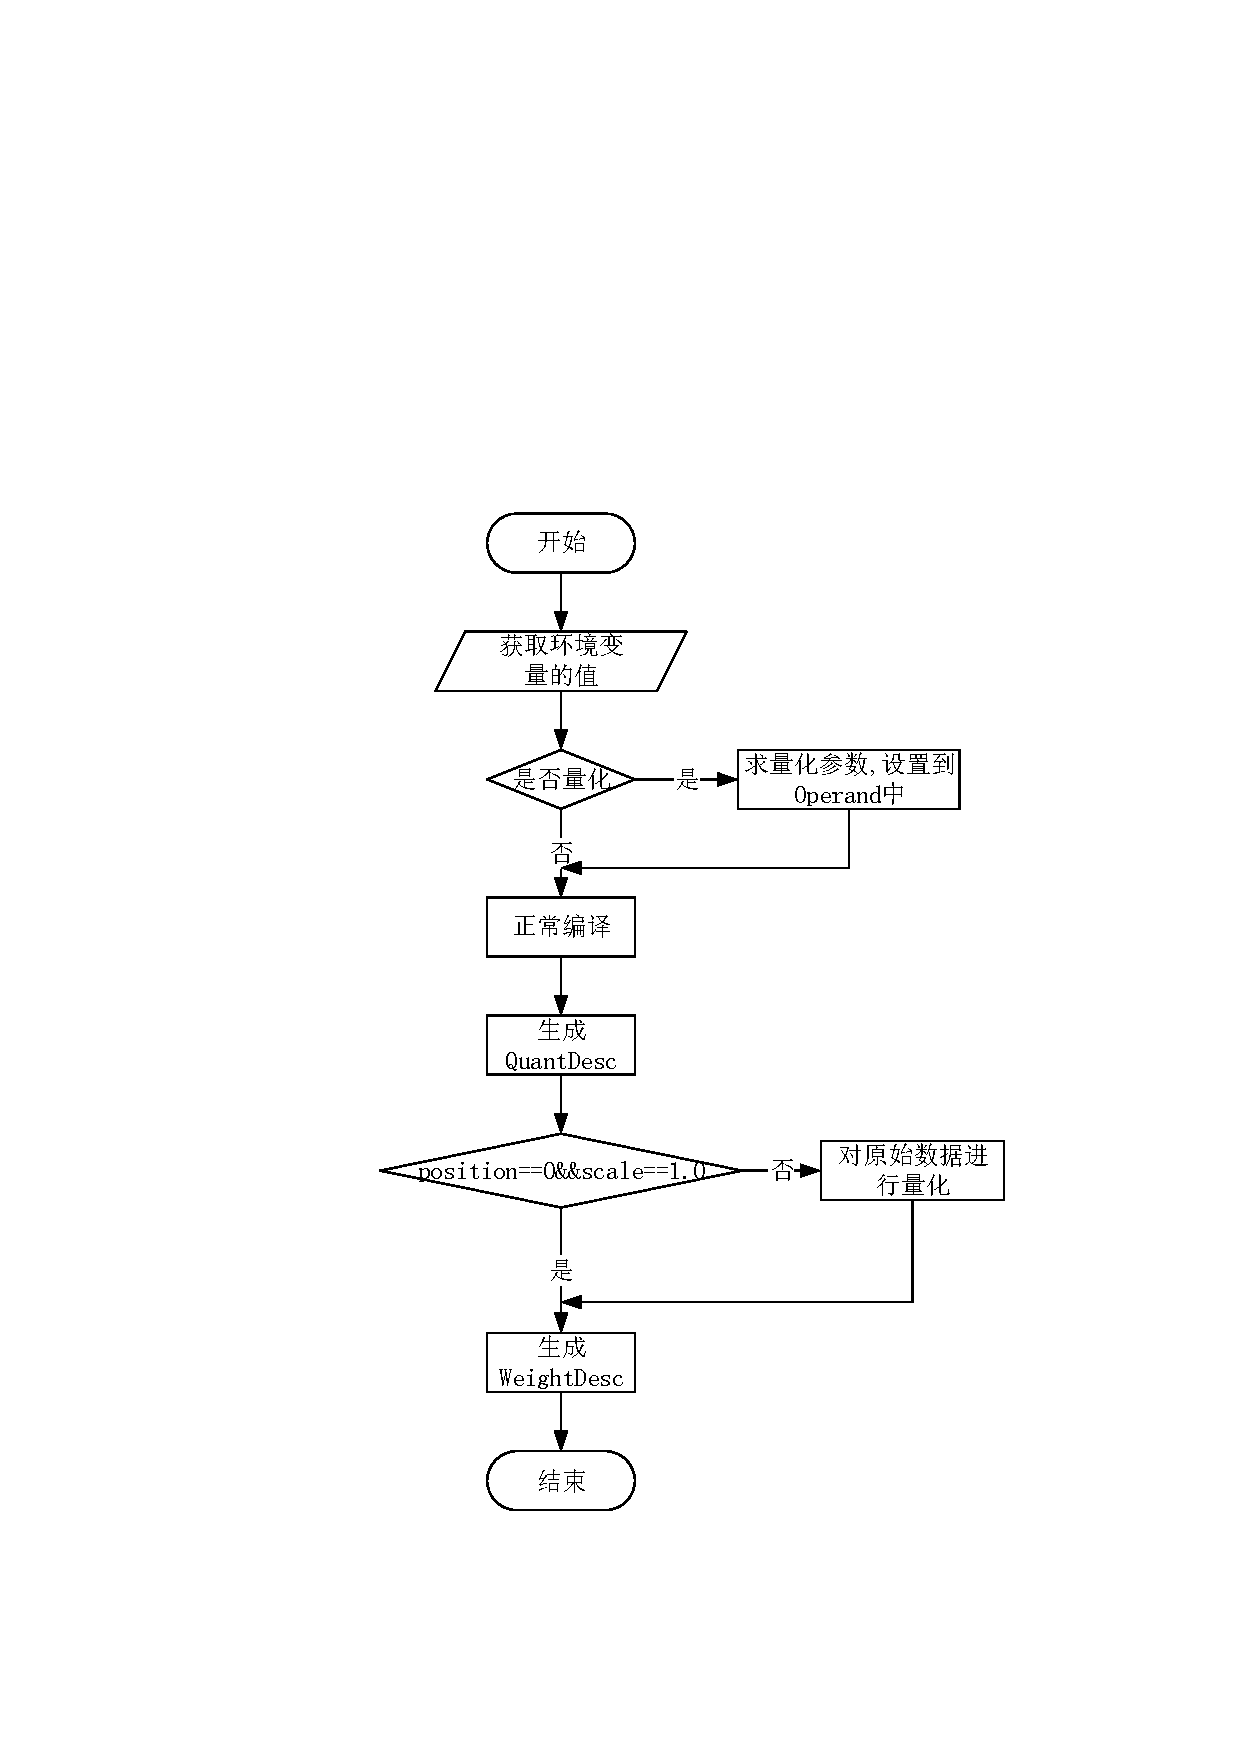
\includegraphics[width=0.4\textwidth]{weight_quant_process.pdf}
  \caption{权值量化流程图}
  \label{fig:weight-quant-process}
\end{figure}

在整个编译生成Kernel的过程中,在两处进行了是否量化的判断,一开始是在编译一开始获取用户计算图的过程中,根据环境变量的值进行判断,如果用户开启了权值量化功能,则求出量化参数并保存到对应的张量中。之后在编译后期生成Kernel的WeightDesc的时候,如果采用了权值量化,则需要对原始数据进行量化处理,将量化后的结果保存到WeightDesc的数据域中。

\section {本章小结}

本章以类图为主,详细介绍了各个模块的实现方式,类之间的关系和接口调用,对于某些比较的复杂的接口,利用流程详细描述其实现逻辑和细节。为了将重点放在模块功能的实现上,在某些模块的设计中,忽略某些不必要的细节,从而突出整体的流程和实现。
% !TeX root = ../main.tex

\chapter{系统测试}
本章在DNNCL的基础上,对比采用运行时优化手段和不采用优化手段时的性能差异,验证优化技术的有效性和实用性。

\section{测试环境}
\subsection {测试方法}
本系统开发完成之后,采用黑盒与白盒测试相结合的方式,对设计的功能模块进行测试,验证系统功能的正确性。然后和优化之前的情况对比,验证系统的实用性。

\subsection{测试环境配置}
测试环境配置信息见表~\ref{tab:experiment-env}。

\begin{table}[htb]
  \centering\small
  \caption{测试配置信息说明}
  \label{tab:experiment-env}
  \begin{tabular}{ll}
    \toprule
    类别       & 配置信息   \\
    \midrule
    硬件环境   & 基于inter-x86结构的CPU \\
              & 主频≥2.4GHz       \\
              & 内存≥4G     \\
              & 硬盘空间≥10G \\
              & DianNao系列MLU100深度学习处理器 \\
    软件  & Ubuntu16.04 \\
          & DNNCL \\
          & DN\_CAFFE  \\
    网络通信  & 无 \\ 
    \bottomrule
  \end{tabular}
\end{table}

\section {性能测试}
测试所用的数据来自于ImageNet数据集,从中随机挑选了5万张带标识的图片用于测试分类网络。在进行性能测试时,每次测试5000张图片,测量10次,然后取加权平均值。

\subsection {指令缓存性能测试}
测试用例设计,指令缓存功能主要是避免重复编译,所以测试用例设计如下。,开启指令缓存功能后,用同一个网络,先后运行三次,第一次记录原始编译过程的时间;第二次开启离线模型缓存功能,记录原始编译加上保存离线模型的时间,观察新加入的过程对总流程有多大的影响;第三次,理论上能正确命中,记录命中之后总的编译时间。对比神经网络的原始编译时间、编译加保存离线模型时间,和命中后编译所需的时间,以检验命中之后是否确实避免了耗时久的编译过程;对比使用离线模型时的正确率和不用离线模型的正确率是否有差异,以检验离线缓存功能对神经网络的结果是否影响。最后用多种不同的网络进行测试,检验功能的完备性和鲁棒性,测试结果如表~\ref{tab:experiment-cache-data}所示。

\begin{table}[htb]
  \centering\small
  \caption{指令缓存测试数据}
  \label{tab:experiment-cache-data}
  \begin{tabular}{llllllll}
    \toprule
    网络      & 原始编译 & 编译加保存 &命中后编 & 第一次&正确率 &第二次&正确率 \\
              & 时间    &模型时间    &译时间   & top1 & top5  &top1 & top5   \\
    \midrule
    Resnet18  & 640.076 & 756.91  & 95.928  & 66.51 & 87.46 & 66.51 & 87.46 \\
    Resnet34  & 1090.24 & 1284.82 & 157.66  & 71.10 & 90.03 & 71.10 & 90.03  \\
    Resnet50  & 3112.29 & 3254.73 & 189.187 & 73.01 & 91.07 & 73.01 & 91.07  \\
    Resnet101 & 7075.01 & 7421.33 & 306.75  & 74.36 & 91.90 & 74.36 & 91.90  \\
    Resnet152 & 12211.2 & 12817.4 & 481.026 & 74.79 & 92.19 & 74.79 & 92.19  \\
    Vgg16     & 1562.58 & 1717.09 & 928.119 & 70.85 & 88.68 & 70.85 & 88.68  \\
    Vgg19     & 1873.26 & 2003.45 & 941.409 & 70.25 & 89.76 & 70.25 & 89.76  \\
    AlexNet   & 938.387 & 1119.93 & 423.322 & 57.13 & 80.21 & 57.13 & 80.21  \\
    GoogleNet & 1275.37 & 1334.38 & 53.8    & 68.75 & 88.37 & 68.75 & 88.37  \\
    MobileNet & 1466.71 & 1531.22 & 51.619  & 70.81 & 89.85 & 70.81 & 89.85  \\
    SequeezeNet & 747.705  & 907.378 & 298.191 & 57.07 & 80.01 & 57.07 & 80.01 \\
    Inception\_V3 & 2875.93 & 3025.54 & 165.192 & 78.23 & 94.20 & 78.23 & 94.20  \\
    \bottomrule
  \end{tabular}
  \note{注:表中编译时间单位为秒;正确率为百分数;top1表示预测的最高值直接命中,top5表示预测的前五个最高值中包含正确结果}
\end{table}

从表中时间数据可知,保存离线模型时会在原来的编译过程中会稍微增加一点时间开销,但是影响不大,影响最大的是Resnet18网络,保存离线模型的时间占到了原始时间的18.25\%,影响最小的是Resnet152网络,保存离线模型的时间子相当于原始时间的4.96\%。然而,网络模型一旦命中,确实可以极大的缩短再次编译的时间,命中后,在次编译时间缩短最大的是Resnet152网络,只有原始编译时间的3.94\%;提升最小的是Resnet18网络,但是也只有原来的14.99\%。所以模型缓存功能可以极大的缩减再次编译的时间,而且数据表明,神经网络越大,原始编译时间越长,则保存模型对原来编译时间的影响越小,模型缓存对编译时间的提升越明显。

从表中正确率数据可知,直接编译运行的正确率和加载缓存的离线模型的正确率没有任何区别。所以存储后再解析加载执行的模式对神经网络的正确率没有任何影响。

\subsection {权值量化性能测试}
权值量化的主要功能是对神经网络的权值数据进行量化处理,在存储是的时候减小存储空间,在运算的时候,利用定点数计算,提升运算速度,加速神经网络的推理过程。权值量化可以加速神经网络的推理过程,但是在一定程度上会降低神经网络的精确度。可以通过量化到不同的精度的方式,来寻求速度和精确度的平衡。由于实验阶段,硬件运算器的限制,只支持量化到Int8类型,所以测试数据只测试了量化到Int8类型时的模型大小、推理时间、已经网络模型的正确率。

量化到Int8类型网络离线模型的大小如表~\ref{tab:experiment-quant-data}所示。

\begin{table}[htb]
  \centering\small
  \caption{指令缓存测试数据}
  \label{tab:experiment-quant-data}
  \begin{tabular}{llll}
    \toprule
    网络      & 量化前模型大小 & 量化后模型大小 & 体积压缩比 \\
    \midrule
    Resnet18  & 17  & 9.6 & 1.77  \\
    Resnet34  & 35  & 19  & 1.84  \\
    Resnet50  & 35  & 20  & 1.75  \\
    Resnet101 & 73  & 37  & 1.97  \\
    Resnet152 & 181 & 63  & 2.87  \\
    Vgg16     & 187 & 134 & 1.40  \\
    Vgg19     & 269 & 211 & 1.27  \\
    AlexNet   & 44  & 39  & 1.13  \\
    GoogleNet & 16  & 6.6 & 2.42  \\
    MobileNet & 14  & 4.9 & 2.86  \\
    SqueezeNet& 3.4 & 1.8 & 1.89  \\
    Inception\_v3  & 49  & 18  & 2.72 \\
    \bottomrule
  \end{tabular}
  \note{注:表中模型大小单位是M(兆)}
\end{table}

由于编译之后保存的离线模型的大小和输入数据的规模(输入数据的规模,间接影响权值等数据的规模)有关,所以不同网络之间的大小会和网络的深度存在一定的差异,但是这并不影响我们比较定点量化网络模型的压缩的功效。从表中我们可以看出,使用定点量化之后的,神经网络模型存储空间大小都得到了较大程度的缩减。压缩比(压缩前的体积/压缩后的体积)最大的是Resnet152,压缩之后只有原来的34.8\%;效果最差的AlexNet网络也只有原来的88.64\%。所以可以说权值压缩可以极大的缩减模型的大小,节省存储空间。

\subsection {权值量化精度测试}

原始的float16网络的和量化后Int8网络的推理时间,以及正确率如表~\ref{tab:quant-result-data}所示。推理性能用单位时间能够处理图片的数量来表示,单位时间内能处理的图片数量越多,则吞吐量越高,计算越快。

\begin{table}[htb]
  \centering\small
  \caption{量化前后测试结果}
  \label{tab:quant-result-data}
  \begin{tabular}{llllllll}
    \toprule
    网络      & 推理性能& &       &正确率 & & &              \\
              &量化前 &量化后 &提升  &top1 & top5 &top1 &top5  \\ 
    \midrule
    Resnet18  & 1741.00 & 2103.00 & 20.79\%  & 66.51 & 87.46 & 66.23 & 87.60  \\
    Resnet34  & 1022.33 & 1302.67 & 27.36\%  & 71.10 & 90.03 & 70.93 & 89.95  \\
    Resnet50  & 645.67  & 781.33  & 21.01\%  & 73.01 & 91.07 & 72.91 & 91.05  \\
    Resnet101 & 369.33  & 465.33  & 25.99\%  & 74.36 & 91.90 & 74.12 & 90.37  \\
    Resnet152 & 261.33  & 326.00  & 24.75\%  & 74.79 & 92.19 & 73.98 & 91.64   \\
    Vgg16     & 289.00  & 416.67  & 44.18\%  & 70.85 & 88.68 & 70.37 & 88.53  \\
    Vgg19     & 214.00  & 335.00  & 56.54\%  & 70.25 & 89.76 & 69.79 & 89.03  \\
    AlexNet   & 996.33  & 1466.33 & 47.17\%  & 57.13 & 80.21 & 56.73 & 79.96  \\
    GoogleNet & 1307.67 & 1335.33 & 2.11\%   & 68.75 & 88.37 & 68.23 & 88.01  \\
    MobileNet & 1633.33 & 1734.33 & 6.18\%   & 70.81 & 89.85 & 69.53 & 88.76  \\
    SqueezeNet & 1842.67 & 2125.67 & 15.36\% & 57.07 & 80.01 & 56.43 & 79.21  \\
    Inception\_v3 & 855.00 & 929.67  & 8.73\% & 78.23 & 94.20 & 78.02 & 93.89  \\
    \bottomrule
  \end{tabular}
  \note{注:推理性能衡量单位image/sec:图片/每秒, 正确率单位:\%}
\end{table}

从表中数据可知,大部分网络在量化之后吞吐量都能得到较大提升,在20\%左右,效果最好的是VGG网络,吞吐量增加了50\%左右。而且正确率并没有出现大幅下降,和量化之前的差距基本在0.5\%左右。

\section {结论}
指令缓存功能命中后可以极大的缩短二次编译的时间,避免重复编译。在缓存空间设置合理的情况下,采用先进先出的原则,可以增加缓存的命中率。权值量化功能不仅能减小神经网络模型编译之后的存储体积,还能大幅度的增加推理速度,提高IO量。在神经网络正确率方面的影响也比较小,在精度要求不高的环境下,基本可以忽略。




% !TeX root = ../main.tex

\chapter{总结与展望}

\section{本文工作总结}
本文对比研究了多个深度学习加速库的编程模型和运行流程,分析深度学习加速库的整体架构,从而提出优化运行时这一关键瓶颈的想法。之后在 DNNCL的基础上,立足于运行时优化的需求分析,详细介绍了整个优化系统和各个模块之间的概要设计和详细设计,给出了主要模块和功能的处理流程和类图以及各个模块详细的设计思路。本文不仅仅是笔者对自身工作的总结,也为后续的研究和开放人员提供了方向和宝贵的参考资料。

本文的主要工作有以下几个方面:
\begin{enumerate}
    \item 本文说明了面向深度学习加速库运行时优化技术的重要意义和作用,详细概括了现代深度学习库的“细腰”结构和设计理念。基于这种结构和设计理念,为提高深度学习库的表现提供了一些优化方向和思路。
    \item 面向优化深度学习加速库的运行时阶段进行需求分析,挖掘系统需求,确定优化系统需要实现什么,具有什么样的功能。
    \item 设计和实现深度学习加速库的运行时优化系统,完成各个模块的开发,支持优化的功能。主要特点在于:本文提出了逆向还原用户计算图结构的想法,并给出了利用JSON 文件保存计算图结构的实现方法,可拓展性良好,支持各种上层框架,适用于各种硬件环境;文中设计了一种离线保存指令模型的文件结构并加以实现,支持模型离线保存和动态加    载,为神经网络模型在嵌入式设备上的部署提供了一种新的方向;基于计算图识别和指令的离线保存,提出了指令缓存的想法,避免使用相同神经网络结构的应用程序的重复编译,大大缩短了应用程序的编译时间,提高了运行效率;将神经网络的结构和权值信息分开保存,结合权值更新技术,提高了缓存的命中率;为了减少神经网络模型的存储空间,提出利用   权值量化来压缩神经网络模型的方法,保证精度损失在可接受范围内可大大减少模型的存储空间。
\end{enumerate}

总而言之,本课题设计和实现基于深度学习加速库运行时的优化系统,采用指令缓存、权值更新等手段来尽量减少神经网络的编译时间,优化编译过程;采用权值量化技术来减少模型的体积,提高存储空间的利用率。

\section{展望}
目前本系统对编译阶段的优化是从宏观上避免相同网络的重复编译,但是对于新出现的网络结构,还是需要经过完整的编译过程,时间较长,对编译的内部流程没做优化处理。目前系统中整张图的编译,是按照调度之后给出的拓扑序进行编译的。其实不连通的子图之间的编译是互不依赖的,可以将整张图按照连
通性进行拆解,分成多张图利用多线程进行分别编译,将会减少编译时间。

在构建阶段没做优化处理,实际上在构建阶段的内部可以做图优化,除了像TensorRT 那样将固定的垂直结构融合成一个层,在多核的情况下,应该还可以将计算图水平拆分,例如将一个大的 conv 拆分成几个小的 conv,每个小的 conv处理其中的一部分,在拼接处的数据用特殊的算子进行处理。这样就可以将一个大的算子拆成几个可以并行执行的小的算子提高计算任务的并行度,从而加快网络的推理过程。

在神经网络加速库的内存管理中,可以增加内存复用模块,在推理过程中,某些使用完的数据是可以释放,不需要一直占用内存空间的,在为后面的数据分配地址的时候,可以考虑复用之前分配过的地址空间。如果不采用内存复用,所需要的内存空间可能是所有数据量的总和,使用内存复用,需要的空间理想情况下是共享数据的最大值。
\bibliography{bib/ustc}

\appendix
% \input{chapters/complementary}

\backmatter
\cleardoublepage
% !TeX root = ../main.tex

\begin{acknowledgements}
时光飞逝如白驹过隙,转眼间两年的研究生生涯即将结束。在这里,我感谢帮助过我,鼓励过我的每一个人。

首先,感谢我的母校中国科学技术大学,感谢科大给了我读研深造的机会,让我有机会遇见那么多优秀的同学,优秀的老师。感谢科大所有教过我或者没有教过我的老师,他们在教学和工作中对学生认真负责的态度给我留下了深刻的印象,至今还记得赵振刚老师指导我们实验课的情形。最重要的是感谢吴峰老师,作为我的校内导师,吴老师不仅忙于教学任务、知道学生和自己的科研工作,还在百忙之中抽出时间指导我的论文,为我的开题报告和论文撰写提出很多有建设性的意见。吴老师学术严谨、工作认真负责,衷心祝贺他永远健康快乐,工作顺利。

其次,要感谢寒武纪公司,给了我实习的机会,让我有机会见识到人工智能从底层硬件设计到上层软件生态系统建设的整个流程,寒武纪公司速度、创新、客户、激情、质量的公司文化一直感染着我。感谢我的企业导师武志辉、郭崎、吴林阳、杜伟健、林楠,感谢他们在工作中给予我的指导和帮助,为我解决了很多工作的疑惑,是我的技术得到了提升。感谢边毅同学,带我看代码,让我能快速的上手工作;感谢杜伟健和吴林阳老师,让我了解公司软件栈的整体架构,让我对任务不在迷茫;感谢武志辉老师,教我合理安排工作和生活,制定目标,激励自己不断进步;感谢我们小组的同学和同事,从他们的代码中我学习到很多,同时也谢谢他们帮忙维护我写的代码,为我提出修改意见
。
当然,还要感谢我的家人和朋友,感谢他们在背后一直支持和鼓励我,遇到挫折,心情低落的时他们为我加油,让我从低落的情绪中重新走出来。感谢父母对我的栽培和默默付出,希望他们永远健康快乐。

最后,感谢所有优秀学者的辛勤耕耘,你们的学术贡献为我的论文提供了启发和思路。感谢所有评审老师给予的批评和指正。

\end{acknowledgements}

\cleardoublepage
%% !TeX root = ../main.tex

\begin{publications}

\section*{已发表论文}

\begin{enumerate}
\item A A A A A A A A A
\item A A A A A A A A A
\item A A A A A A A A A
\end{enumerate}

\section*{待发表论文}

\begin{enumerate}
\item A A A A A A A A A
\item A A A A A A A A A
\item A A A A A A A A A
\end{enumerate}

\section*{研究报告}
\begin{enumerate}
\item A A A A A A A A A
\item A A A A A A A A A
\item A A A A A A A A A
\end{enumerate}

\end{publications}


\end{document}
